
\documentclass[oneside]{ausarbeitung}
\bibliography{latexlit.bib}


% ----------------------------------------------------------------------

\begin{document}

%--- Sprachauswahl
% Erlaubte Werte:
%   \selectlanguage{english}
%   \selectlanguage{ngerman}
\selectlanguage{ngerman}

%--- Art der Arbeit
% Erlaubte Werte:
%   \Praxissemesterbericht
%   \Projektbericht
%   \Bachelorarbeit
%   \Seminararbeit
%   \Masterarbeit

\Projektbericht

%--- Studiengang:
% Erlaubte Werte:
%   \Informatik
%   \Elektronik
%   \DataScience
\Informatik

\title{Entwicklung einer Augmented Reality Applikation zur Wiedererkennung bereits eingelernter Objekte}

\author{Michael Schlosser}
\matrikelnr{75984}

%--- Ist der Erstbetreuer (\examinerA) an der Hochschule ein Professor?
% Erlaubte Werte:
%   \examinerIsAProfessortrue   % Ja
%   \examinerIsAProfessorfalse  % Nein

\examinerIsAProfessorfalse % Nein
%--- Betreuer
\examinerA{~Dr.~Marc~Hermann}
%\examinerB{Prof.~Dr.~Ulrich~Klauck}

%--- Einreichungsdatum
\date{\today}

%--- Angaben zur Firma
% Auskommentieren, wenn die Arbeit nicht bei einer ext. Firma gemacht wurde.
%\companyname{Beispielfirma}
%\industrialsector{Beispielbranche}
%\department{Beispielabteilung}
%\companystreet{Beispielstr. 1}
%companycity{12345 Musterstadt}

%--- Angaben zum Betreuer bei dieser Firma
%\advisorname{Name des Betreuers}
%\advisorphone{(01234) 567-890}
%\advisoremail{name@company.xxx}

%--- Titelseite Anzeigen
\maketitle
\cleardoublepage

%---
\pagenumbering{roman}
\setcounter{page}{1}

%--- Firmendaten Anzeigen
% Auskommentieren, wenn die Arbeit nicht bei einer ext. Firma gemacht wurde.
%\makeworkplace
%\cleardoublepage

%--- Eidesstattliche Erklärung anzeigen
\makeaffirmation
\cleardoublepage

%---
\begin{abstract}
	Das Einlernen und Wiedererkennen von beliebigen Objekten ist im Bereich des Maschinellen Sehens immer noch ein aktuelles und noch nicht gänzlich erforschtes Thema. Ein exemplarischer Anwendungsfall hierfür, wäre dem Nutzer die Möglichkeit zu bieten durch eine Kamera ein Objekt einzulesen und das Kamerabild bei Erkennung des Objektes mit bildunterstützenden Elementen zu ergänzen.\\
	Die geringe Rechenleistung von Mobile und Embedded Devices stellt jedoch den Einsatz dieser Technologie auf diesen Geräten vor eine Herausforderung. Verschiedene Ansätze, um die Rechenintensität eines Einlern-/ und Wiedererkennungsalgorithmus gering zu halten, sind bereits verfügbar und einsetzbar. \\
	Eine weitere Schwierigkeit, die sich beim kontinuierlichen Einlernen von Objekten ergeben kann, ist das bekannte Phänomen des Katastrophalen Vergessens, welches dafür sorgt, dass beim Trainingsvorgang bereits eingelernte Objekte mit neuen überschrieben werden.\\
	Im Rahmen dieser Arbeit wird eine Android-Applikation für mobile Endgeräte entwickelt, welche den im obigen beschriebenen Anwendungsfall erfüllen kann. Zum Einlernen und Wiedererkennen werden bereits trainierte Deep Learning Architekturen mithilfe der Methode \glqq Continual Learning\grqq\ erweitert, um die Kernfunktionalität erbringen zu können.
\end{abstract}
%-----------------------------------------------------------------------
\cleardoublepage
\tableofcontents

%---
\listoffigures

%---
\listoftables

%---
\lstlistoflistings

%---
\listofabbreviations
\begin{acronym}[Bsp.]  % Längstes Kürzel in der nachfolgenden
                       % Liste um die Breite der Spalte für die
                       % Abkürzungen zu bestimmen.

%% Eintrag: \acro{Referenzname}[Kürzel]{Langform}
%% Im Text wird die Abkürzung dann mit \ac{Referenzname} benutzt.
\acro{api}[API]{Application Programming Interface}
\acro{art}[ART]{Android Runtime}
\acro{ac}[AR]{Augmented Reality}
\acro{blob}[Blob]{Binary Large Object}
\acro{cnn}[CNN]{Convolutional Neural Network}
\acro{dcnn}[DCNN]{Deep Convolutional Neural Network}
\acro{dnn}[DNN]{Deep Neural Network}
\acro{dsc}[DSC]{Depthwise Separable Convolution}
\acro{ml}[ML]{Machine Learning}
\end{acronym}
%---


\cleardoublepage
\pagenumbering{arabic}
\setcounter{page}{1}

% ----------------------------------------------------------------------
\chapter{Einleitung}
\label{cha:einleitung}
Das Einlernen und Wiedererkennen von Objekten kann in vielen Bereichen Anwendung finden, wie beispielsweise in der Tourismus- oder Videospielbranche, sowie auch in der Medizin und Rüstungsindustrie. Die Nutzung von Deep-Learning-Algorithmen hat sich als \textit{state-of-the-art} im Bereich der Bildklassifizierung etablieren können. Bei diesem Ansatz werden mit einer enormen Anzahl von Trainingsdaten sogenannte Neuronale Netze für ein bestimmtes Anwendungsgebiet trainiert.\\
Deep Learning wurde bereits in den frühen 50er Jahren erforscht, bei der Simulation von Neuronen im menschlichen Gehirn, um generelle Lernprozesse besser verstehen zu können. Aufgrund der enormen Rechenleistung, die aufzubringen ist, fand der Ansatz erst später wieder Anklang im Bereich des Maschinellen Lernens, da die Hardware die zur Verfügung steht, immer leistungsstärker wird \cite{dl-review}. Gleichzeitig werden im Bereich der Robotik und dem Internet der Dinge, die Verwendung von eingebetten Systemen und Mikroprozessoren und die Verwendung von Smartphones immer gefragter. Um einen effizienten Klassifizierungsalgorithmus implementieren zu können ist demnach eine möglichst kleine Deep Learning Architektur zu verwenden.\\
Der in dieser Ausarbeitung gegebene Anwendungsfall unterscheidet sich jedoch vom eben beschriebenen Ansatz des Trainings und dem Einsatz von Klassifizierungsalgorithmen. Der gewöhnliche Arbeitsablauf für die Bereitstellung einer Klassifizierungsapplikation wäre ein Training bestehend aus einer erheblichen Anzahl an Trainingsdaten auf einem rechenstarken Computer zu vollziehen. Anschließend würde ein vollständig trainiertes Netz nicht mehr weitertrainiert werden, sondern lediglich versuchen Objekte aufgrund des stattgefundenen Trainings korrekt klassifizieren zu können. In dieser Ausarbeitung ist jedoch ein Netz noch nicht endgültig trainiert worden und weitere Objekte sollen vom Nutzer eingelernt werden können. Dies erfordert den Trainingsalgorithmus auch auf leistungsärmeren Geräten, welche für den Einsatz der Technologie genutzt werden, zur Verfügung zu stellen.\\
Im Rahmen dieser Projektarbeit wird eine Applikation für ein Android-Smartphone entwickelt, welche die Funktionalität des Einlernens und Wiedererkennens bereitstellen kann. Hierfür werden diverse Technologien und Ansätze im Grundlagenkapitel aufgearbeitet, welche zum Verständnis dieser Ausarbeitung essentiell sind. Anhand dieser Grundlagen ist eine Softwarearchitektur zuerst im Groben und daraufhin in Form eines Feinentwurfs zu designen. Die Applikation soll daraufhin implementiert und getestet werden.
% ---
\chapter{Grundlagen}
\label{cha:grundlagen}
Zur Lösung der Problemstellung sind verschiedene Grundlagengebiete zu beherr-
schen, die zum einen bereits im Rahmen des Informatikstudiums verinnerlicht werden konnten und zum anderen Gebiete und Themen, die erst im Laufe der Recherche und Implementierung der Projektarbeit erarbeitet worden sind.
\section{Deep Neural Networks}
Konventionelle Methoden des Maschinellen Lernens sind in der Verarbeitung von rohen Daten, wie beispielsweise den Pixeln von Bildern, ineffizient.
Deep Learning bezeichnet ein Teilgebiet des Maschinellen Lernens, welches in diesen Anwendungsfällen eine bessere Alternative darstellt. Ein \ac{dnn} ist ein mehrschichtiges Rechenmodell, welches sich vor allem in den Gebieten der Bild- und Spracherkennung als \textit{state-of-the-art} etablieren konnte.\\
Beim Deep Learning wird zwischen Training und Inferenz unterschieden. Beim Training werden in das Netz annotierte Trainingsdaten gegegeben, welche vom Netz prozessiert werden. Daraufhin werden die Gewichte des Netzes kalibriert um die Merkmale der eingelesenen Trainingsdaten wiedererkennen zu können.\\
Beim Vorgang der Inferenz erzeugt das Netz eigenständig Ausgaben. Der produktive Einsatz von \acp{dnn} entspricht demnach dem Vorgang der Inferenz \cite{deepl-vs-traditional, deepl-lecun}. 
\subsection{Deep Convolutional Neural Networks}
Bei den meisten Bildklassifizierungs- und Objektdetektionsapplikationen werden sogenannte Faltungsschichten (\textit{engl.: Convolutional Layers}) verwendet, da sich diese als sehr effizient in diesem Anwendungsfall erweisen konnten.\\
In der Mathematik bezeichnet eine Faltungsschicht das Überlappen zweier Funktionen.\\
Eine Faltungsschicht besteht aus sogenannten Convolutional Filters mit der Größe $D_K \times D_K \times M$ wobei $D_K$ der Höhe und Breite des Filters und $M$ der Anzahl an Kanälen beziehungsweise der Tiefe des Filters entspricht. Der Filter gleitet nun über das Eingabebild $F$ und multipliziert $F$ mit dem Filter. Die Ergebnisse dieser Multiplikation werden als Skalarprodukt zu einem Wert zusammengefasst. Nachdem der Filter über alle Pixel des Bildes gegleitet ist ergibt sich eine neue kleinere Matrix, welchere als gefaltetes Merkmal (\textit{engl.: Convolved Feature}) bezeichnet wird.
\subsection{Mobilenet}
Bei der rapiden Weiterentwicklung von \ac{dnn}-Architekturen wird das Augenmmerk stets auf die Verbesserung der Genauigkeit des Modells gelegt. Da die Latenzzeit und Größe des Netzes zunehmen, ist der Einsatz auf Geräten mit limitierter Rechenleistung für Echtzeitsysteme nur schwer möglich.\\
Mobilenets sind \acp{dnn}, die speziell für Aufgaben im Bereich des Maschinellen Sehens auf mobilen Endgeräten und eingebetteten Systemen entwickelt wurden. Ein Mobilenet Modell basiert auf sogenannten \acp{dsc}, welche die Faltungsschichten in einem \ac{dcnn} hinsichtlich der Netzgröße und Inferenzzeit optimieren. \\
Der Rechenaufwand beim Prozessieren einer Faltungsschicht ist durch die hohe Anzahl an nötigen Multiplikationen enorm. \acp{dsc} berechnen die Faltung in mehreren Phasen. In der ersten Phase wird die sogenannte Tiefenfaltung angewendet, welche die herkömmliche Faltung lediglich auf einem Kanal berechnet. In der zweiten Phase wird die sogenannte Punktfaltung angewendet, wobei die Merkmale aus der Tiefenfaltung miteinander kombiniert werden. Dies verringert den Rechenaufwand deutlich.\\
Der Aufbau des Mobilenet v2, welches Anwendung im gegebenen Anwendungsfall findet, wird in Abbildung \ref{fig:mobilenet-architecture} dargestellt \cite{mobilenet}.
\begin{figure}[hptb]
	\centering
	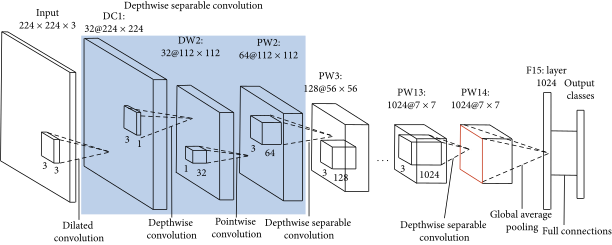
\includegraphics[height=0.27\textheight]{images/mobilenet-architecture.png}
	\caption{Architektur eines Mobilenet v2} Quelle: https://www.hindawi.com/journals/cin/2020/8817849/fig2/ abgerufen am 30.07.2021
	\label{fig:mobilenet-architecture}
\end{figure}

\subsection{Imagenet}
Imagenet ist ein frei verfügbarer Datensatz bestehend aus 14.197.122 annotierten Bildern, welcher seit 2010 für die \textit{Imagenet Large Scale Visual Recognition Challenge} (ILSVRC), einem Benchmark für Bildklassifizierung und Objektdetektion, genutzt wird \cite{imagenet}. Ein derart riesiger Datensatz ist für das möglichst generische Einlernen von neuen unterschiedlichen Objekten jeglicher Art von Vorteil, da sich dieser Datensatz nicht auf ein bestimmtes Themengebiet bezieht, wie beispielsweise der Bildklassifizierung von Objekten im Straßenverkehr oder der Klassifizierung von bestimmten Haushaltgegenständen. \\
\section{Wiedererkennung von Objekten}
\label{sec:basics:wiedererkennung}
Das Einlernen und Wiedererkennen von Objekten ist im Bereich des Maschinelles Lernens noch heute eine Herausforderung für eingebettete beziehungsweise mobile Endgeräte, aufgrund der geringen Rechenleistung, die zur Verfügung steht. Es ist möglich diese Aufgabe mithilfe einer Cloudlösung auf einen externen leistungsstarken Server zu übertragen. Aufgrund von Nachteilen, wie beispielsweise Sicherheitsrisiken, die beim Übertragen von sensitiven Daten auftreten, wird im Rahmen dieser Arbeit eine Applikation programmiert, die den gegebenen Anwendungsfall mit der dem Endgerät zur Verfügung stehenden Hardware löst.\\
Ein naiver Ansatz, um dieses Problem lösen zu können ist ein  \ac{cnn} bei Eingang neuer Trainingsdaten erneut zu trainieren mitsamt den bereits vorhandenen Daten. Ein derart riesiger Lernvorgang ist jedoch nicht praktikabel und könnte mehrere Stunden oder sogar Tage dauern. Wenn lediglich die neuen Daten für das Training verwendet werden, resultiert dies im bekannten Phänomen des \textit{Katastrophalen Vergessen} \cite{Senchanka2019}.
\subsection{Katastrophales Vergessen}
Neuronale Netze tendieren dazu beim Einlernen von aufeinanderfolgenden unterschiedlichen Aufgaben das bereits gelernte Wissen zu vergessen. Dieses Phänomen wird als Katatrophales Vergessen beziehungsweise als \textit{Katastrophale Inferenz} bezeichnet. Die Ursache hierfür ist, dass Gewichte von Neuronen, die für eine vorherige Aufgabe wichtig sind, überschrieben werden, um die neue eingelernte Aufgabe zu erfüllen \cite{forgetting}.\\
Für den gegebenen Anwendungsfall bedeutet dies, dass alte bereits eingelernte Objekte nicht mehr erkannt werden können, wenn ein bereits trainierter Datensatz mit unbekannten Daten weitertrainiert wird. Lösungsansätze für dieses Problem werden im Folgenden erklärt.

\subsection{Transfer Learning}
Jedes menschliche Gehirn, ist dazu fähig Wissen, welches für eine Aufgabe benötigt wird, auf eine andere Aufgabe zu übertragen. So ist es beispielsweise mit geringem Aufwand möglich das Autofahren zu erlernen, wenn man bereits Motorrad fahren kann. Da es eine ähnliche Aufgabe ist, wird nicht versucht die neue Aufgabe von Grund auf neu zu lernen, sondern das Wissen, welches in der Vergangenheit erlernt werden konnte auf ein neuen ähnlichen Anwendungsfall zu transferieren.\\
Im traditionellen Ansatz des Maschinellen Lernens wird ein Datensatz aufbereitet, welcher für eine bestimmte Aufgabe zugeschnitten ist.\\
Die grundlegende Aufgabe, die in dieser Arbeit zu erfüllen ist, ist jedoch das Einlernen von neuen Trainingsdaten. Hierfür kann der Ansatz des sogenannten Transfer Learnings Anwendung finden.\\
Beim Transfer Learning wird ein bereits trainiertes \ac{ml}-Modell verwendet. Das bereits errungene Wissen kann hierbei weiterverwendet werden, um mit einem kleineren Trainingsdatensatz eine neue ähnliche Aufgabe erfüllen zu können. Erkannte Merkmale wie Formen, Kanten und Ecken können demnach durch den Wissenstransfer mit einem Modell geteilt werden. Bei dieser Vorgehensweise werden die unteren Schichten, welche die nicht-klassenspezifischen Merkmale erkennen, eingefroren. Dies bedeutet, dass die Gewichte der Neuronen unveränderbar sind. Die oberen Schichten sind weiterhin trainierbar. Durch Training eines Datensatzes, welcher den neu einzulernenden Daten ähnelt, werden lediglich die klassenspezifischen Merkmale trainiert \cite{Senchanka2019}. In Abbildung \ref{fig:tf-architecture} wird diese Architektur mit dem Traditionellen \ac{ml}-Ansatz verglichen.\\
Wenn stets neue Klassen eingelernt werden sollen und diese Daten sich nicht innerhalb einer Trainingsstapels befinden, tritt jedoch das Phänomen des Katastrophalen Vergessens auf und früher eingelernte Objekte werden überschrieben \cite{cl-vs-tl}.

\begin{figure}[hptb]
	\centering
	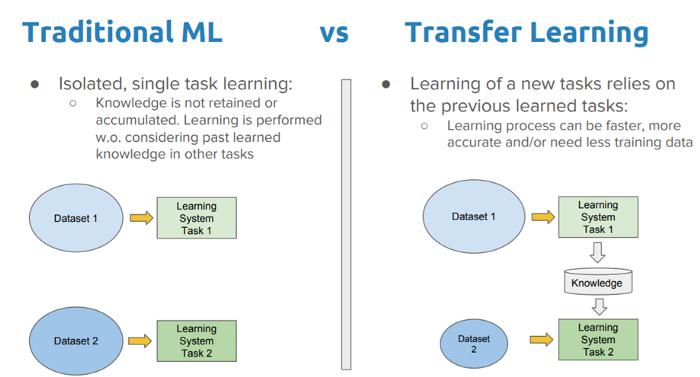
\includegraphics[height=0.4\textheight]{images/traditional-vs-tflearning.png}
	\caption{Vergleich des Aufbaus eines Transfer Learning Models im Gegensatz zum traditionellen Maschinellen Lernen} Quelle: \cite{Sarkar2019}
	\label{fig:tf-architecture}
\end{figure}

\subsection{Latent-Replay-Algorithmus}
Das grundlegende Konzept beim Latent-Replay-Algorithmus bildet das sogenannte \textit{Replay} beziehungsweise \textit{Rehearsal}. Bereits trainierte Trainingsdaten werden hierfür in einem separaten Datenbank persistent gespeichert und bei Eingang neuer Trainingsdaten ebenfalls mitgelernt.
Das Problem hierbei ist jedoch, dass die Trainingsdauer massiv zunimmt, da in jeder Trainingsepoche mehrere Trainingsiterationen durch das Neuronale Netz notwendig sind. Zudem ergibt sich aus dem Abspeichern von alten Trainingsdaten ein Speicherproblem auf eingebetteten Systemen.\\
Der Latent-Replay-Algorithmus erweitert den Ansatz des Rehearsals, um eben diese Schwierigkeiten zu beheben. Hierfür werden nicht rohe Bilddaten abgespeichert sondern Aktivierungen von Neurononen innerhalb einer Schicht der Netzarchitektur. Bei einer Trainingsiteration werden neue Eingangsdaten durch Schichten des Netzen weitergeleitet, welche für das Erkennen von generischen Merkmalen zuständig sind, wie beispielsweise Ecken und Kanten. Anschließend werden diese Daten in die Latent-Replay-Schicht, welche die Speicherung der alten Trainingsdaten übernimmt, weitergeleitet, wobei die Eingangsdaten nun mit den Aktivierungen der alten Trainingsdaten vermischt werden. Die Schichten, die oberhalb der Latent-Replay-Schicht angesetzt sind, sind für die Erkennung von klassenspezifischen Merkmalen zuständig \cite{Pellegrini2019}. In Abbildung \ref{fig:latent-replay} wird der eben erklärte Aufbau dargestellt.\\
Das Prinzip des Transfer Learnings kann dementsprechend mithilfe des Latent-Replay-Algorithmus erweitert werden und dadurch das Phänomen des Katastrophalen Vergessens beheben, durch das Mittrainieren von alten Trainingsdaten.

\begin{figure}[hptb]
  \centering
  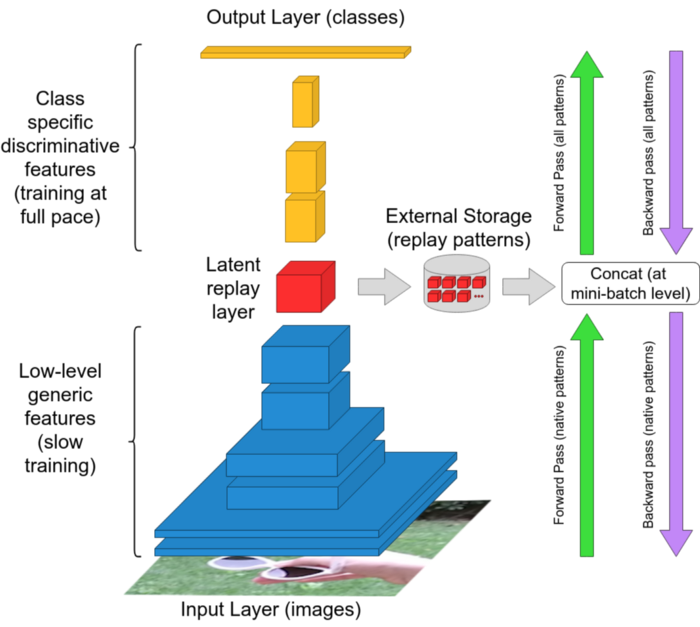
\includegraphics[height=0.4\textheight]{images/latent-replay.png}
  \caption{Architekturdiagramm des Latent Replay} Quelle: \cite{Pellegrini2019}
  \label{fig:latent-replay}
\end{figure}
\section{Android}
Android ist ein auf Linux basierender Open-Source-Software-Stack, der für eine Vielzahl von Geräten entwickelt wurde.\\
Jede Applikation läuft in einer separaten Instanz der \ac{art}, welche dafür konzipiert wurde Applikationen auf Geräten mit geringem Hauptspeicher innerhalb separater virtueller Maschinen auszuführen. Die \ac{art} basiert auf dem Linux-Kernel und ermöglicht es Geräteherstellern Hardware-Treiber für einen bekannten Kernel zu entwickeln.\\
Jede Android Version wird mit einer ganzen Zahl bezeichnet, welche als API-Ebene beziehungsweise API-Level bekannt ist und bei der Entwicklung von neuen Applikationen angegeben werden muss. Um bestimmte Features nutzen zu können, muss die API-Ebene einen bestimmten Wert besitzen. Geräte die nur bis zu einer bestimmten Version kompatibel sind, werden demnach die zu entwickelnde Applikation nicht ausführen können.
\cite{android-platform}
\subsection{Shared Preferences}
Shared Preferences bezeichnen einen Key-Value-Store für primitive Daten in Form einer XML-Datei. Genutzt werden kann dies über die dafür zur Verfügung gestellte Android-Bibliothek, welche ein Shared Preferences-Objekt erzeugt. Dieses Objekt beinhaltet einen Zeiger auf den Pfad der jeweiligen Datei. Mithilfe von Shared Preferences können beispielsweise Konfigurationsparameter, die persistent abgespeichert werden sollen mithilfe einer einfachen \ac{api} zugänglich gemacht werden.
% ---
\chapter{Anforderungsanalyse}
\label{cha:analyse}
Zur Erarbeitung der Anforderungen der gegebenen Aufgabenstellung, werden diese hinsichtlich ihrer Umsetzungsrelevanz gegliedert und gewichtet.
\begin{itemize}
\item \textbf{Must-Have-Anforderungen} sind unbedingt umzusetzen. Sie umfassen die Kernfunktionalitäten, die zur Lösung der gegebenen Aufgabenstellung essentiell sind.
\item \textbf{Should-Have-Anforderungen} beschreiben Eigenschaften des Systems, die vorteilhaft für die Lösung der gegebenen Aufgabenstellung sind und einen großen Mehrwert für die Software bieten, jedoch nicht zwingend erforderlich sind.
\item \textbf{Could-Have-Anforderungen} sind optionale Anforderungen an Eigenschaften des Systems, die ebenfalls einen relevanten Mehrwert bieten können, welcher jedoch nicht zwingend erforderlich für die Lösung der gegebenen Aufgabenstellung ist. 
\item \textbf{Nice-To-Have-Anforderungen} sind ebenfalls optionale Anforderungen an Eigenschaften des Softwaresystems. Diese sind jedoch von untergeordneter Bedeutung.
\end{itemize}
Im Folgenden werden die Anforderungen an das zu entwickelnde Softwaresystem thematisch gruppiert und unterteilt in funktionale und nicht-funktionale Anforderungen.
\section{Funktionale Anforderungen}
Funktionale Anforderungen erklären, welche Funktionen und Dienste vom Software-System bereitzustellen sind und insbesondere die Beziehungen zwischen den Ein- und Ausgabedaten.

\subsection{Lauffähigkeit als Android-App}
Eine auf einem aktuellen Android-Betriebssystem lauffähige Applikation soll entwickelt und auf einem Smartphone in den Betrieb genommen werden. Es wird gefordert, dass der Nutzer des Software-Systems die im Smartphone integrierte Kamera nutzt und diese als Eingabe für das Einlernen und die Wiedererkennung eines Objektes nutzt.  -- \textit{Gewichtung:} Must-Have-Anforderung.
\subsection{Entwicklung einer graphischen Benutzeroberfläche}
Es wird gefordert eine Graphische Benutzeroberfläche zur Verfügung zu stellen, mit welcher der Nutzer interagieren kann. Der Touchscreen des Smartphones sollte das Haupteingabegerät des Nutzers zur Steuerung der Applikation sein. -- \textit{Gewichtung:} Must-Have-Anforderung.
\subsection{Einlernen von Objekten mithilfe einer Kamera}
Es wird gefordert, dass ein Objekt mit der integrierten Smartphone-Kamera, bei guten Licht- und Kontrastverhältnissen eingelernt werden kann. Bei erfolgreicher Abspeicherung der Daten, soll dem Nutzer dies mitgeteilt werden. Der Nutzer hat nun die Möglichkeit das eingelernte Objekt mit Daten zu versehen, wie beispielsweise einem Namen. Die Informationen über das nun eingelernte Objekt werden in einer Datenbank persistent abgespeichert, um sie wieder abrufen zu können. -- \textit{Gewichtung:} Must-Have-Anforderung.

\subsection{Wiedererkennung bereits eingelernter Objekte mithilfe einer Kamera}
Ein bereits eingelerntes Objekt soll bei guten Licht- und Kontrastverhältnissen vom Softwaresystem in Echtzeit wiedererkannt werden. -- \textit{Gewichtung:} Must-Have-Anforderung.

\subsection{Markierung der wiedererkannten Objekte}
Wenn ein Objekt von der Applikation erkannt wird, soll es beispielsweise durch das Einblenden des Namens des Objektes dem Nutzer mitgeteilt werden, dass das eingelernte Objekt wieder auf dem Display des Smartphones zu sehen ist. -- \textit{Gewichtung:} Should-Have-Anforderung.
\subsection{Graphisches Overlay bei wiedererkannten Objekten}
Die für das eingelernte Objekt gespeicherten Daten sollen als ein graphisches Overlay auf dem Bildschirm des Smartphones dargestellt werden, wenn das Objekt erneut erkannt worden ist. -- \textit{Gewichtung:} Must-Have-Anforderung.

%
\section{Nicht-funktionale Anforderungen}
% Wie gut soll das System das leisten? 
Im Folgenden werden die Einschränkungen und Qualitätsmerkmale an die Entwicklung und den Betrieb des Systems erklärt.

\subsection{Lauffähigkeit auf einem Smartphone}
Die Kompatibilität und ein angemessenes Laufzeitverhalten auf einem aktuellen Android-basierten Smartphone wird gefordert, um eine benutzerfreundliche Applikation bereitstellen zu können. -- \textit{Gewichtung:} Must-Have-Anforderung.

\subsection{Dauer und Umstände des Erlernens der Objekte}
Ein Objekt soll bei guten Lichtverhältnissen in annehmbarer Zeit eingelernt werden. -- \textit{Gewichtung:} Must-Have-Anforderung.

\subsection{Benutzerfreundlichkeit}
Die Graphische Benutzeroberfläche ist so intuitiv wie möglich zu gestalten, um die Bedienung des Systems ohne größeren Einarbeitungsaufwand erlernen zu können. -- \textit{Gewichtung:} Should-Have-Anforderung.

\subsection{Wartbarkeit und Erweiterbarkeit}
Änderungen und Erweiterungen des Software-Systems sollten mit hinnehmbarem Aufwand bewerkstelligt werden können. Demnach sollte der Quellcode modular, strukturiert und dokumentiert sein. -- \textit{Gewichtung:} Should-Have-Anforderung.

\section{Anwendungsfälle}
Die zu entwickelnde Applikation soll dem Hauptakteur \glqq User\grqq\ die in Abbildung \ref{fig:usecase-diagram} dargestellten Anwendungsfälle erfüllen können. Eine genaue Beschreibung wurde in Anhang \ref{appendix:use-cases} verlagert, um den Lesefluss nicht zu stören. 
\begin{figure}[hptb]
	\centering
	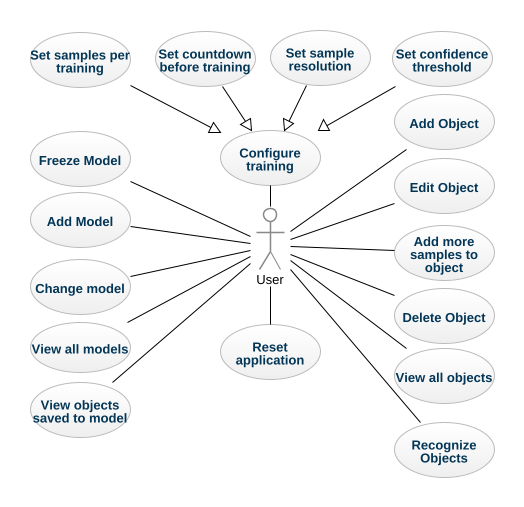
\includegraphics[height=0.6\textheight]{images/usecase-diagram.png}
	\caption{UML-Anwendungsfall-Diagramm} Quelle: Eigene Darstellung
	\label{fig:usecase-diagram}
\end{figure}
%---
\chapter{Entwurf}
\label{cha:Entwurf}
Auf der Basis der im vorangegangenen Kapitel erstellten Anforderungsanalyse 
und der im Grundlagenkapitel aufgearbeiteten theoretischen Kenntnisse 
wird im Folgenden ein Lösungskonzept erarbeitet.
\section{Grundlegende Designentscheidungen}
Die für den Entwurf der Applikation zugrundelegenden Entscheidungen, welche für die erfolgreiche Implementierung entscheidend sind, werden im Folgenden erklärt.
\subsection{Tensorflow Lite und Continual Learning}
Tensorflow Lite ist ein Open-Source Deep Learning Framework, welches für die Inferenz von Deep Learning Modellen auf Mobilen Endgeräten und eingebetteten Systemen entwickelt wurde \cite{tflite-site}.\\
Aufgrund einer bereits vorhandenen Beispielimplementierung einer Transfer Learning Applikation, wurde eine Basis für die ersten Ansätze einer Anbindung der Wiederkennungsfunktionalität unter der Nutzung von Transfer Learning für die Applikation, die in dieser Projektarbeit zu entwickeln ist, geschaffen.
Tensorflow Lite stellt eine \ac{api} zur Verfügung, welche die Nutzung von Transfer Learning vereinfacht. Zudem ist es durch ein Python-Skript möglich selbst generierte Tensorflow Lite-Modelle für das Transfer Learning vorzubereiten.\\
Bei dem in diesem Projekt verwendeten Modell handelt es sich um eine Mobilenet V2 Architektur, welche auf dem Imagenet-Datensatz trainiert wurde, um ein breites Spektrum verschiedener Klassen erkennen zu können mit einem möglichst geringen Rechenaufwand.\\
Um einen Latent-Replay Algorithmus in die Applikation zu übertragen, wurden Anpassungen vorgenommen nach dem Vorbild von Demosthenous et al. \cite{cl-vs-tl}, welche im Rahmen ihrer Forschung den Transfer Learning Ansatz mit dem Continual Learning Ansatz von Pellegrini et al. \cite{Pellegrini2019} verglichen haben.
\section{Entwurfsmuster}
Um sich auf bereits bewährte Entwurfsansätze bestehender Software beziehen zu können, werden unter anderem mehrere Entwurfsmuster aus dem \textit{GoF-Buch} genutzt. Dies ermöglicht es qualitativ hochwertige Software zu entwickeln, welche durch das Anwenden von allgemein bekannten Mustern von anderen Entwicklern leichter nachvollzogen werden kann.
\subsection{Ports-und-Adapter}
Um ein möglichst wart- und erweiterbares Softwareprodukt zu entwickeln, wurde das \textit{Ports-und-Adapter-Muster}, soweit dies möglich war, angewendet, um Third-Party-Dependencies, wie beispielsweise Tensorflow Lite, aber auch um die Persistenz möglichst abstrakt zu halten und eine Bindung an konkrete Implementierungen und Technologien zu vermeiden. Dies erhöht die Testfähigkeit enorm, da das \textit{Dependency-Inversion-Prinzip} angewendet wird und die Abhängigkeiten der Geschäftslogik so gering wie möglich gehalten werden .

\subsection{Factories}
Um die Erzeugung von Objekten ähnlicher Klassen, wie beispielsweise Dialogboxen, möglichst konsistent zu halten, werden diese mithilfe des \textit{Factory}-Musters erstellt, soweit dies möglich war.

\subsection{Observer}
Um eine starke Kopplung der Komponenten zu vermeiden, wird das \textit{Observer}-Muster so weit dies möglich ist verwendet. Es findet vor allem im Aktualisieren der Graphischen Oberfläche, aber auch bei der Interkommunikation von entkoppelten Dialogfenstern und Fragments, sowie bei der Beobachtung von asynchronen Prozessen Anwendung.

\subsection{Fragments}
Da das Entwickeln einer Android-Applikation zu den Anforderungen gehört, ist zu entscheiden, ob man eine Applikation auf Basis mehrerer Android-Aktivitäten  (\textit{engl.: Activities}) erstellt, oder eine Activity mithilfe von angefügten sogenannten Fragmenten (\textit{engl: Fragments}) entwickelt. Das Nutzen von Fragments ermöglicht die Interkommunikation der Systemkomponenten über die Activity, zu welcher diese gehören. Da in mehreren Anwendungsfällen das Zusammenarbeiten mehrerer Systemkomponenten notwendig ist, ist die Nutzung von Fragments der Nutzung von mehreren Aktivitäten vorzuziehen.\\
Die Oberfläche der Applikation kann mithilfe von XML-Code generiert werden. Programmatisch wird die Oberfläche an die Funktionalität, welche in Java-Code geschrieben wurde, gebunden.\\


\section{Entitätsklassen}
\label{cha:design:entities}
Die für die Geschäftslogik grundlegenden und technisch unbedingt notwendigen Entitäten werden in Abbildung \ref{fig:er-diagram} dargestellt. In den folgenden Unterkapiteln werden diese erläutert.\\
Zu allen Entitäten wird eine einzigartige fortlaufende Identifikationsnummer (ID) gespeichert.
\begin{figure}[hptb]
	\centering
	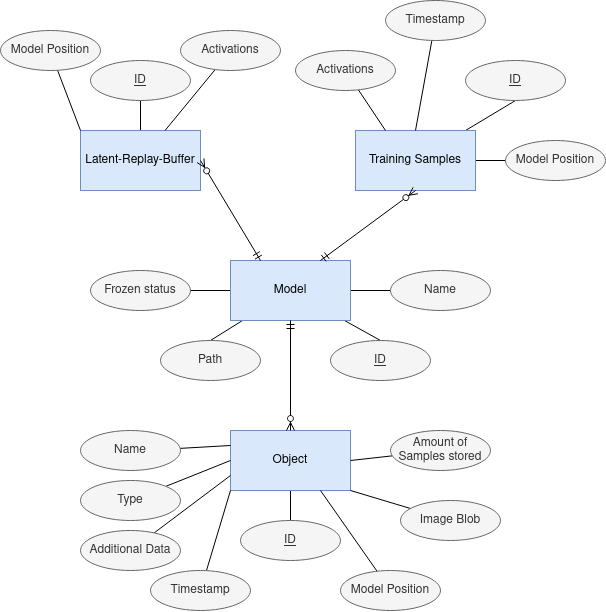
\includegraphics[height=0.6\textheight]{images/er-diagram.png}
	\caption{Entity-Relationship-Diagramm} Quelle: Eigene Darstellung
	\label{fig:er-diagram}
\end{figure}

\subsection{Modell}
Um dem Nutzer eine Unterscheidungsmöglichkeit zu bieten wird zu dem Modell ein Name abgespeichert.\\
Der absolute Pfad zu einer lokalen Binärdatei, die die derzeitige Parametrisierung des Modells festlegt wird zusätzlich abgespeichert, anstatt die Binärdaten direkt als \ac{blob} zu speichern. Dies vereinfacht es die Applikation bei Bedarf um eine \glqq Modell teilen\grqq-Funktion zu erweitern. \\
Zusätzlich wird ein boolescher Wert zu jedem Modell abgespeichert, welcher entscheidet, ob das Modell bereits eingefroren wurde, um den Nutzer warnen zu können, wenn er im Begriff ist bereits bestehende Objekte aufgrund des Phänomen des Katastrophalen Vergessen zu überschreiben.
\subsection{Objekt}
Das Objekt ist die Kernentität der Applikation. Im Rahmen dieser Projektarbeit wurden einem Objekt diverse Attribute, wie beispielsweise dem Objekttyp oder dem generischen Attribut \glqq Weitere Daten\grqq\ angefügt. Es ist jedoch möglich die zusätzlichen Daten, außer dem bezeichnenden Objektnamen, leer zu lassen, da diese keine Auswirkungen auf die Funktionsweise der Applikation haben.\\
Jedes Objekt hat eine Beziehung zu einem bestimmten Modell. Dies kann durch das Speichern einer Modell-Identifikationsnummer als Fremdschlüssel realisiert werden.\\
Ein Modell stellt eine Anzahl an Endknoten zur Verfügung, welche sich direkt auf die Endknoten der Netzarchitektur des zugrundeliegenden \ac{dcnn} projizieren lassen. Demnach ist zu jedem Objekt eine Modelposition zu speichern. Anhand dieser Kartierung ist eine lose Kopplung zwischen Objekt und Modell und eine generische Erstellung von beliebig vielen Modellen und demnach beliebig vielen Objekten, anknüpfend an bestimmte Modelle, möglich.\\ 
Außerdem wird dem Objekt automatisch ein Zeitstempel hinzugefügt, um dem Nutzer darüber Auskunft geben zu können, wann das jeweilige Objekt eingespeichert wurde. Zudem ist ein Zeitstempel für mögliche weitere Datenabfragen und beispielsweise Erweiterungen der Objektübersicht mit einer Nach-Datum-Sortierungsfunktion sinnvoll.\\
Sobald ein Objekttraining gestartet wird, wird die erste Bitmap, die in der Trainings-Vorbereitungs-Pipeline eingeht persistent abgespeichert, um dem Nutzer eine Vorschau des Objektes zu geben, falls es in Vergessenheit geraten ist, um welches Objekt es sich handelt.\\
Die Speicherung der Anzahl der Trainingsdaten pro Objekt sind von monitorischer Bedeutung. Durch das Speichern und die spätere Anzeige dieser Daten kann der Nutzer entscheiden, ob es sinnvoll ist einem Objekt weitere Trainingsdaten hinzuzufügen. Mögliche Erkennungsprobleme wie beispielsweise einer ungleichen Verteilung an Trainingsdaten können dadurch leichter festgestellt werden.\\
\subsection{Trainingsdaten}
Die Aktivierungen im Bottleneck-Layer des zugrundeliegenden Mobilenet v2, werden persistent abgespeichert, mitsamt der jeweiligen Modellposition und der Modell-Identifikationsnummer, zu welchem die Trainingsdaten gehören. Erforderlich ist dies aufgrund der Implementierung eines Continual Learning Ansatzes unter Verwendung des Latent-Replay Algorithmus, da alte Trainingsdaten bei einem Objekttraining vermischt werden, um das Phänomen des Katastrophalen Vergessens zu lösen.\\
Ein Zeitstempel wird zu jedem Trainingsdatenfeld hinzugefügt, um lediglich die letzten $n$ Daten in den Latent-Replay-Puffer zu überführen.
\subsection{Latent-Replay-Puffer}
Der Latent-Replay-Puffer wird nach jeder Trainingssitzung aktualisiert mit den zuletzt hinzugefügten Trainingsdaten.\\
Zudem wird die Modellidentifikationsnummer als Fremdschlüssel und die Modellposition, zu welchem das jeweilige Trainingsdatenfeld gehört mitabgespeichert, um das Vermischen von neuen Trainingsdaten und alten Trainingsdaten, nach dem Prinzip des Latent-Replay-Algoritmhus zu ermöglichen.
\section{Architektur}
\label{cha:architecture}
Zur Realisierung der Applikation auf einem Android-Endgerät, werden die Komponenten der zugrundelegenden Architektur aus Activities und Fragments bestehen. Eine Activity-Komponente wird für den Startbildschirm erstellt, welche die Haupt-Activity für die Funktionalität der App einleitet. Mithilfe von Fragments, die an diese Activity anknüpfen kann die Kommunikation und der Datenaustausch zwischen verschiedenen Fragments stattfinden.\\
Abbildung \ref{fig:component-diagram} zeigt die Abhängigkeiten der im Folgenden erklärten verwendeten Komponenten.\\
Im Folgenden werden die Verantwortlichkeiten der zu implementierenden Fragments erklärt und die Anwendungsfälle aus Anhang \ref{appendix:use-cases} werden zugewiesen.

\begin{itemize}
	\item \textit{Model Overview Fragment}: Dient der Übersicht über alle Modelle, sowie der Möglichkeit, die Objekte die im jeweiligen Modell gespeichert sind anzuschauen. Zudem kann in diesem Fragment ein weiteres Modell hinzugefügt werden, oder das aktuell ausgewählte Modell mit einem ebenfalls bereits bestehenden Modell ausgewechselt werden. Demnach werden die Anwendungsfälle M1-M4 von dieser Komponente erfüllt.

	\item \textit{Object Overview Fragment}: Dient der Übersicht über alle Objekte und deren gespeicherten Informationen, sowie der Möglichkeit Objekte zu editieren und zu löschen. Zudem soll dem Fragment die Verantwortlichkeit hinzugefügt werden, dem jeweiligen Objekt weitere Trainingsdaten hinzuzufügen. Demnach werden die Anwendungsfälle O3-O6 von dieser Komponente erfüllt.
	
	\item \textit{Settings Fragment}: Konfigurationen, die der Nutzer selbst zur Laufzeit vornehmen kann, werden innerhalb dieses Fragments in einer typischen Einstellungen-Ansicht realisiert. Demnach werden die Anwendungsfälle E1-E5 von dieser Komponente erfüllt. Weitere Konfigurationsmöglichkeiten zur Verfügung zu stellen, wie zum Beispiel das Aktivieren eines Dunkelmodus ist ebenfalls geplant.
	
	\item \textit{Camera Fragment}: Stellt die Hauptfunktionalität des Einlernens und Wiedererkennens zur Verfügung. Eine Kameravorschau, die mit einer Fokusbox und anderen Overlays, die zum Anzeigen von Informationen dienen, ausgestattet ist, soll in Echtzeit aktualisiert werden. Eine Dialogbox wird zum Einlernen eines Objektes aufgerufen, um diesem optional Informationen hinzufügen zu können. Innerhalb dieses Fensters wird der Trainingsvorgang initiiert. Demnach werden die Anwendungsfälle O1 und O2 von dieser Komponente erfüllt.
	
	\item \textit{Help Fragment}: Falls bei der Bedienung der Applikation Schwierigkeiten auftreten sollten, stellt das Help Fragment diverse Anleitungen und Nutzungsabläufe textuell dar.

\end{itemize}

Durch Anwendung dieser Architektur, wird die sogenannte \textit{separation of concerns} gewährleistet und das \textit{Single-Responsibility-Principle} angewendet.\\
Weitere Komponenten sind der Datenbankhelfer, welcher eine zu implementierende Schnittstelle an die Applikation zur Realisierung von Persistenz-Operationen beinhaltet. Implementiert werden, kann diese Schnittstelle beispielsweise von einem SQLite-Datenbankhelfer.\\
Zur globalen Konfiguration verschiedener Parameter, welche auch nach Neustart der App vorhanden sein sollen, wird ebenfalls eine Schnittstelle zur Verfügung gestellt, welche beispielweise durch Verwendung der \textit{Shared Preferences} implementiert werden kann.\\
Um die Übersichtlichkeit und der darausfolgenden besseren Wart- und Testbarkeit der Applikation zu gewährleisten, werden Dialogboxen ausgelagert und mithilfe einer Schnittstelle und einer \textit{Factory-Method} erzeugt. Dialogboxen werden zur Interaktion mit dem Nutzer häufig verwendet. Das Hinzufügen oder Ändern von Daten, sowie das Anzeigen von längeren Hinweisen wird über Dialogboxen an den Nutzer kommuniziert. Bei gefährlichen Aktionen, wie beispielsweise dem Löschen von Objekten oder dem Zurücksetzen der Applikation wird der Nutzer ebenfalls durch eine Dialogbox auf die möglichen Auswirkungen der Aktion hingewiesen.\\
Statische Methoden, die dem Parsen von Zeichenketten, oder dem Vorbereiten der Kameradaten an die Transfer Learning \ac{api} dienen, werden in eine \textit{Utilities}-Komponente ausgelagert, um den Code, der die Kernfunktionalität realisiert möglichst übersichtlich und kompakt zu halten.\\
Die Anbindung der \textit{Transfer Learning \ac{api}} erfolgt in Form einer Wrapper-Klasse, welche die \ac{api} um weitere Verantwortlichkeiten erweitert, wie beispielsweise dem Kontinuierlichen Trainieren und Wiedererkennen innerhalb einer While-Schleife und dem Ausführen des Latent-Replay Algorithmus. Aufgrund der Ausführung des Algorithmus muss eine Abhängigkeit zur Schnittstelle des Datenbankhelfers erfolgen, da die persistente Abspeicherung von Aktivierungen früherer Trainingsdaten unabdingbar für den Replay-Vorgang ist. Zudem übernimmt der Wrapper die Erstellung des Modells und koordiniert die \ac{api} an die Parameter-Datei des ausgewählten Modells.
\begin{figure}[hptb]
	\centering
	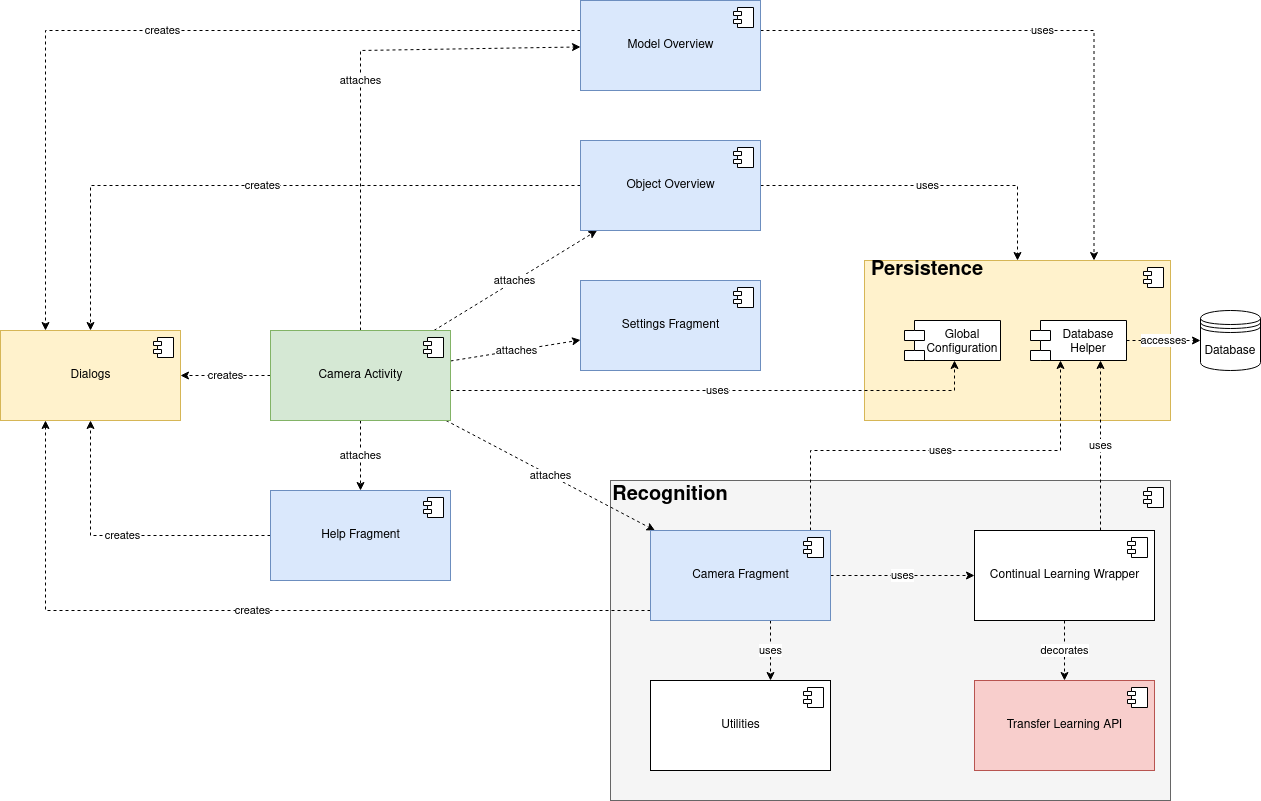
\includegraphics[height=0.5\textheight]{images/building-block-view.png}
	\caption{UML-Komponentendiagramm} Quelle: Eigene Darstellung
	\label{fig:component-diagram}
\end{figure}

\section{Feinentwurf}
Im Folgenden werden die Strukturen und Abläufe, der in Kapitel \ref{cha:architecture} beschriebenen Komponenten erklärt.\\
Um eine Übersichtlichkeit der Klassendiagramme zu gewährleisten, wurden nicht alle Methoden und Komponenten aufgeführt. Die Lücken werden mit der Zeichenfolge \glqq\ ... \grqq\ gekennzeichnet.
\subsection{Klassendiagramme}
Im Folgenden wird die statische Struktur der Komponenten auf Klassenebene erklärt.
Um eine Übersichtlichkeit des Entwurfes gewährleisten zu können, werden Komponenten nach ihren Verantwortlichkeiten und erfüllten Anwendungsfällen getrennt beschrieben.
\subsubsection{Persistenz-Komponente}
Die Persistenz des Objektes wird mithilfe von Schnittstellen angebunden und lässt sich in eine Komponente für Globale Konfigurationsparameter und eine Komponente für die Anbindung einer Datenbank aufteilen. Die Datebankhelfer-Schnittstelle stellt Methoden zur Abfrage, Einfügen und Löschen der strukturiert gespeicherten Entitätsklassen zur Verfügung. In der Schnittstelle für die globalen Konfigurationsparameter, werden Methoden zur Verfügung gestellt, die primitive Daten, die persistent für Abläufe der Applikation gespeichert werden müssen, abgefragt und gespeichert.\\
Abbildung \ref{fig:class-diagram-persistence} zeigt den Aufbau der Komponenten auf Klassenebene und deren Beziehungen zu anderen Komponenten.
\begin{figure}[hptb]
	\centering
	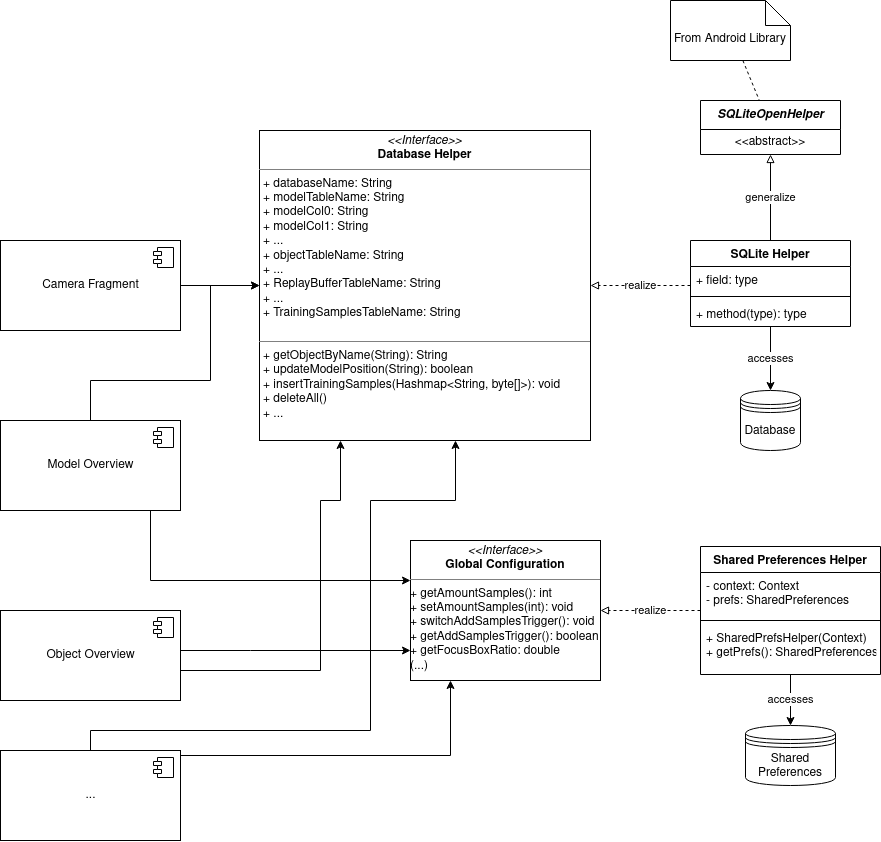
\includegraphics[height=0.6\textheight]{images/persistence-class-diagram.png}
	\caption{UML-Klassendiagramm der Persistenz Komponente} Quelle: Eigene Darstellung
	\label{fig:class-diagram-persistence}
\end{figure}
Durch die Verwendung von Schnittstellen wurde das Dependency Inversion Principle angewendet. Bei Bedarf ist es dadurch möglich die SQLite Datenbank durch eine andere auszutauschen unter der Bedingung, dass alle Methoden der Schnittstelle implementiert werden.
\subsubsection{Kamera Fragment}
Das Kamerafragment enthält Methoden zur Ansteuerung des Continual Learning Modell Wrappers und zur Konfiguration und Vorbereitung der Kameradaten. Zudem werden die in der Datenbank gespeicherten Objekte an die Endknoten des Modells angeheftet, um bei einer Wiedererkennung die Daten des Objektes wiederanzeigen lassen zu können.\\ 
Aufgrund des Einsetzens des MVVM-Patterns wird ein Viewmodel für das Fragment aggregiert, welches unter Verwendung von Livedaten die Graphische Oberfläche kontinuierlich aktualisiert. Die Livedaten werden hierbei innerhalb eines anonymen Observers, welcher in der von Fragment geerbten \glqq \textit{onViewCreated}\grqq-Methode erzeugt werden.\\
Um den Wertebereich des Trainingsstatus zu optimieren, wird eine Enumeration mit den Status \glqq Noch nicht gestartet \grqq, \glqq Gestartet \grqq\ und \glqq pausiert\grqq\ eingebunden.\\
Um die Daten in Echtzeit und eine möglichst nicht blockierende Applikation zu schreiben, wird eine Unterklasse zum Hinzufügen von Trainingsdatenanfragen als Thread ausgeführt, welche zudem einen Countdown vor dem Starten der Methode zum Trainingsdaten hinzufügen ausführt.\\
Der Continual Learning Model Wrapper erweitert die von Tensorflow Lite zur Verfügung gestellte Transfer Learning \ac{api}, um den Latent-Replay-Algorithmus und Methoden um die Modellparameter in einer separaten Datei abzuspeichern und zu laden.\\
Die Transfer Learning \ac{api} stellt die wichtigsten Methoden für das Training, die Inferenz und dem Speichern und Laden von Parameterdaten zur Verfügung.

\begin{figure}[hptb]
	\centering
	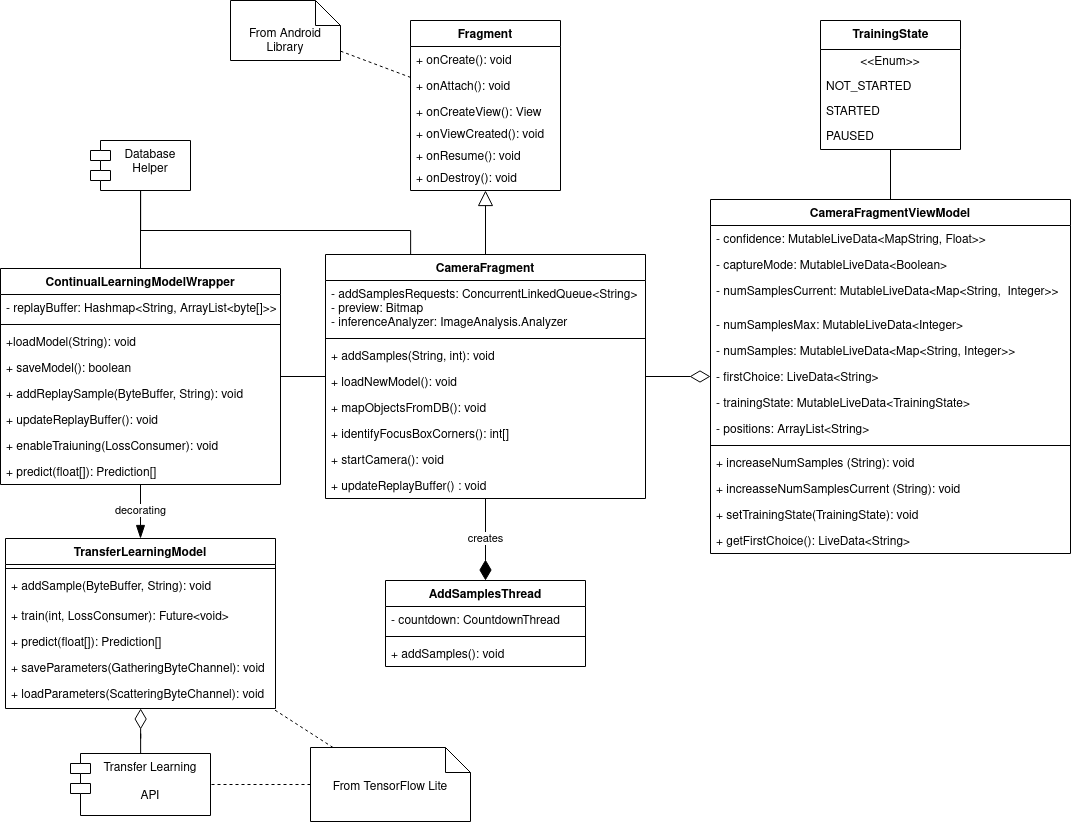
\includegraphics[height=0.55\textheight]{images/camera-fragment-class-diagram.png}
	\caption{UML-Klassendiagramm der Wiedererkennungs-Komponente} Quelle: Eigene Darstellung
	\label{fig:recognition-classdiagram}
\end{figure}
\subsubsection{Modell- und Objektübersicht}
Da die Modell- und Objektübersicht analog aufgebaut sind, wird die Beschreibung der Komponenten auf Klassenebene in einem einzigen Unterkapitel vereint.\\
Die Verbindung zur Persistenzkomponente ermöglicht es die Listeninstanzen mit Daten aus der Datenbank zu füllen. Zur Erstellung einer angepassten Listenansicht wurde der Listenadapter von Android erweitert. Dieser Listenadapter bietet die Möglichkeit eine Listenansicht zu Erstellen, anhand der Position der zu identifizierenden Elemente. Dadurch können Listelement-spezifische Daten an die Methoden übergeben werden. Ein Beispiel hierfür ist das Einfügen von Click-Listenern auf Buttons, welche anhang dieser Position angesteuert werden. Das Dialog-Paket wird ebenfalls genutzt und fördert somit die Wiederverwendbarkeit der Komponenten. Abbildung \ref{fig:overview-classdiagram} zeigt die statische Struktur der Modell- und Objektübersicht auf Klassenebene.
\begin{figure}[hptb]
	\centering
	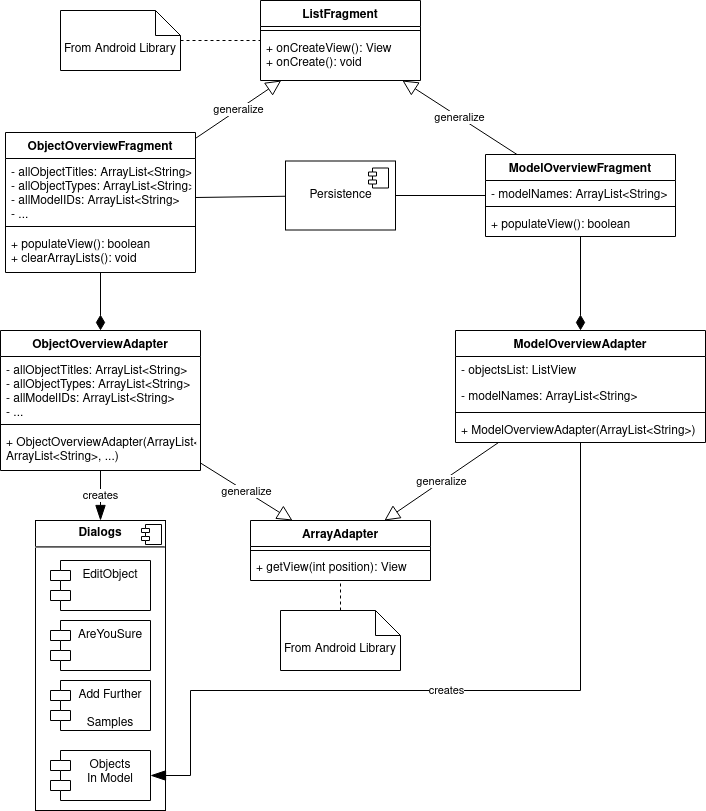
\includegraphics[height=0.7\textheight]{images/object-overview-class-diagram.png}
	\caption{UML-Klassendiagramm der Objekt- und Modellübersicht} Quelle: Eigene Darstellung
	\label{fig:overview-classdiagram}
\end{figure}
\subsubsection{Dialoge}
Die Dialoge wurden innerhalb eines Paketes gebündelt und werden mithilfe einer statischen \textit{Factory-Method} erstellt. Mithilfe einer Methode zum Erzeugen des Dialoges werden diese für den Nutzer sichtbar.\\
Die Dialoge, die dem Nutzer Hilfestellungen geben, werden im \textit{Help Fragment} aufrufbar sein und werden mithilfe einer generischen Methode initialisiert. Eine abstrakte \textit{Help Dialog}-Klasse stellt die notwendige Logik für Hilfe-Dialoge zur Verfügung. Innerhalb der konkreten Klassen können die einzelnen textuellen Hinweise einer Methode als Argument übergeben werden. \\
Das Help Fragment wird analog zur Modell- und Objektübersicht mit einem angepassten Listenadapter entworfen. Diese Liste wird fest in der Implementierung des Help Fragment initialisiert. Klicks auf das jeweilige Listenelement öffnet den zugehörigen Hilfedialog.\\
Abbildung \ref{fig:dialogues} zeigt den Entwurf des Help Fragments und die statische Struktur des Dialogpakets.
\begin{figure}[hptb]
	\centering
	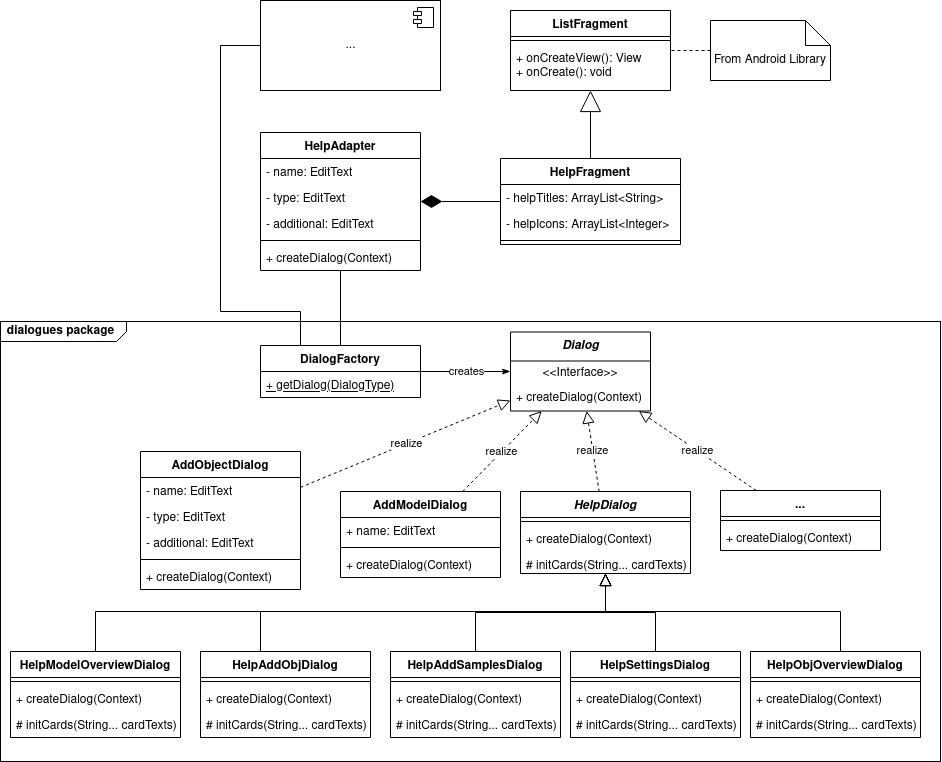
\includegraphics[height=0.6\textheight]{images/dialogues.png}
	\caption{UML-Klassendiagramm der Dialogpakets und des Help Fragments} Quelle: Eigene Darstellung
	\label{fig:dialogues}
\end{figure}
\subsection{Kommunikation der Komponenten}
\label{cha:communication-components}
Die \textit{Camera Activity} ist die Hauptkomponente und bietet die Möglichkeit Informationen und Benachrichtigungen, welche zwischen den Fragmenten erfolgen sollen, auszutauschen. Eine Navigationsleiste am unteren Bildschirmrand und ein aufklappbares Seitenmenü bietet dem Nutzer die Möglichkeit, die angezeigten Fragmente zu wechseln und deren Funktionalität zu nutzen.\\
Die Activity beobachtet bestimmte Aktionen innerhalb der Fragmente, registriert sich als \textit{Observer} bei den Globalen Konfigurationsparametern und koordiniert Befehlsaufrufe an das jeweils benötigte Fragment. Die Komponente zur Globalen Konfiguration wird hierfür von Fragmenten, die interagieren müssen, instanziiert.\\
Abbildung \ref{fig:sequence-diagram-change-model} stellt diesen  Ablauf in Form eines Sequenzdiagrammes, am Beispiel des Änderns des ausgewählten Modells graphisch dar. 

\begin{figure}[hptb]
	\centering
	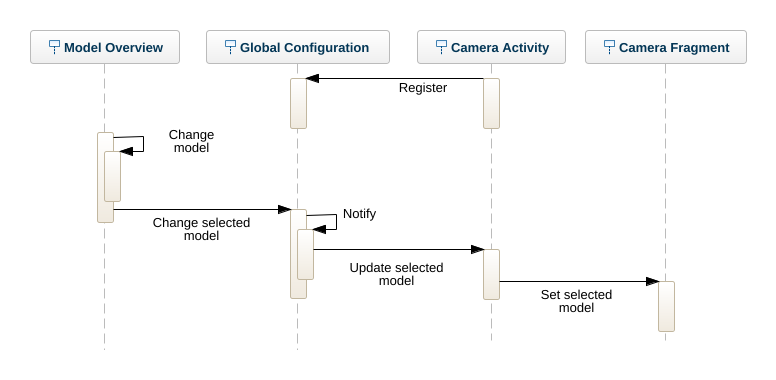
\includegraphics[height=0.35\textheight]{images/sequence-diagram-change-model.png}
	\caption{UML-Sequenzdiagramm: Ändern des ausgewählten Modells} Quelle: Eigene Darstellung
	\label{fig:sequence-diagram-change-model}
\end{figure}

Durch Nutzung dieses Musters ist eine lose Kopplung der Komponenten möglich und Fragmente können ohne voneinander abhängig zu sein ausgeführt werden. Analog zu diesem Beispiel werden die folgenden Abläufe realisiert:
\begin{itemize}
	\item Objekttraining auslösen
	\item Objekttraining Rollback auslösen im Fehlerfall
	\item Aktualisieren des Replay-Puffers
	\item Initialisieren der Namen der Ausgabeknoten des Modells (standardmäßig werden die Ausgabeknoten mit aufsteigenden Nummern als Zeichenkette initialisiert)
	\item Auflösung der Trainingsdaten anpassen
	\item Konfidenzschwelle anpassen
	\item Länge des Countdowns vor dem Training anpassen
	\item Aktivieren des Dunkelmodus
\end{itemize}

\subsection{Vorbereitung und Vorschau der Kameradaten}
Das Camera Fragment beinhaltet eine Vorschau in Echtzeit, welche dem Nutzer ermöglicht zu sehen, was die im Endgerät eingebaute Kamera sieht.\\
Zur Realisierung dieser Funktionalität müssen diverse Konfigurationen vorgenommen werden. Hierzu gehört das Initialisieren der Ausrichtung des Gerätes (Portrait- oder Landscape-Modus), Das Seitenverhältnis, die Auflösung der Kamera und weiteren systembezogenen Einstellungen wie beispielsweise dem automatischen Fokussieren. Zudem wird ein Bildanalyse-Thread zur Vorkonfiguration der Kameraansicht hinzugefügt. Die Inferenz- und Trainingsfunktionalität wird direkt hier eingesetzt, da dies ermöglicht jeden angezeigten Frame asynchron zum Programmablauf zu akquirieren und zu verarbeiten. \\
Nach Konfiguration der soeben beschriebenen Parameter, wird die Kamera an den Lebenszyklus des Fragments gebunden und demnach bei Öffnen des Fragments gestartet und Schließen beziehungsweise Wechseln geschlossen.\\
\subsection{Einlernen von Objekten}
\label{cha:train-objects}
Das Einlernen und Wiedererkennen von Objekten sind die umfangreichsten und komplexesten Anwendungsfälle in der Applikation, welche diverse Komponenten involvieren und Interprozesskommunikation von nebenläufigen Prozessen erfordert.\\
Die Struktur und der Ablauf des in Anwendungsfall \ref{tab:use-case-add-object} beschriebenen sichtbaren Verhaltens, wird im Folgenden präziser erklärt.\\
Nach Betätigung des \glqq +\grqq-Buttons auf der graphischen Oberfläche wird ein Dialogfenster erzeugt. Nach Eingabe der Informationen zum Objekt, löst der \glqq Training starten\grqq-Button im Dialogfenster unter Anwendung des in Kapitel \ref{cha:communication-components} beschriebenen Ablauf das Objekttraining aus. Parallel dazu werden die eingegebenen Daten des Objektes in der Datenbank gespeichert. Die Activity delegiert den Aufruf an das Camera Fragment, welches die Verantwortlichkeiten für das Einlernen trägt. \\
Eine Warteschlange bestehend aus Modellpositionen wird hierbei innerhalb eines neuen Threads mit der vorkonfigurierten Anzahl an Trainingsdaten pro Objekttraining gefüllt.\\
Diese Warteschlange wird kontinuierlich vom Analysierer abgefragt und entscheided dadurch, ob Objekte trainiert, oder lediglich Inferenz ausgeführt werden soll.\\
Der Analysierer bereitet die stets zugeführten Kameradaten im YUV-Format für das Training vor.\\
Beim Vorbereiten der Daten werden die von der Kamera bereitgestellten Daten in Bitmaps umgewandelt und in die Größe der auf dem Bildschirm dargestellten Fokusbox zugeschnitten. Danach wird die Bitmap auf die Größe der Eingangsknoten des Netzes skaliert. Die Bitmap wird anschließend in ein Float-Datenfeld konvertiert, da dies die Datenstruktur ist, mit welchem das zugrundeliegende Deep-Learning-Modell Eingangsbilder prozessiert.\\
Wenn sich in der Warteschlange Trainingsanfragen befinden, wird die eingehende Bitmap zum Objekt dazugespeichert, damit es bei der Wiedererkennung und in der Objektübersicht als Objektvorschau angezeigt werden kann. Das nun vorbereitete Trainingsdatenfeld wird in den Continual Learning Model Wrapper gegeben und zugleich zu den Trainingsdaten in der Datenbank abgespeichert.\\
Der Wrapper leitet das Training an die Transfer Learning \ac{api} weiter, welche das Modell nun für die übergebene Modellposition trainiert.
Dieser Trainingsprozess findet kontinuierlich statt, durch das Starten eines Training-Threads im Wrapper.\\
Parallel dazu wird der Trainingsfortschritt prozentual ermittelt und im View Model aktualisiert. Ein Observer aktualisiert nun während des Trainings einen Ladekreis auf der graphischen Oberfläche.\\
Falls ein Fehlerfall eintritt, wie beispielsweise dem frühzeitigen Wechseln des Fragments, werden die Änderungen in der Datenbank zurückgesetzt und somit das noch nicht fertig trainierte Objekte wieder gelöscht. Zudem wird der Nutzer über seinen Fehler durch eine Meldung informiert.\\

\subsection{Wiedererkennen von Objekten}
Das Wiedererkennen von Objekten findet kontinuierlich statt, wenn die Anfragewarteschlange leer ist. Hierfür wird eine Methode im Modell-Wrapper, welche direkt die Inferenzmethode der Transfer Learning \ac{api} aufruft, ausgeführt. Die Ergebnisse aktualisieren im angebundenen View Model das erkannte Objekt und die Konfidenz dazu. Mithilfe eines Observers wird die graphische Oberfläche kontinuierlich aktualisiert.\\
Die eben erklärten Abläufe zum Einlernen und Wiedererkennen von Objekten, werden in Abbildung \ref{fig:activity-diagram-model} als Aktivitätsdiagramm graphisch dargestellt.
\begin{figure}[hptb]
	\centering
	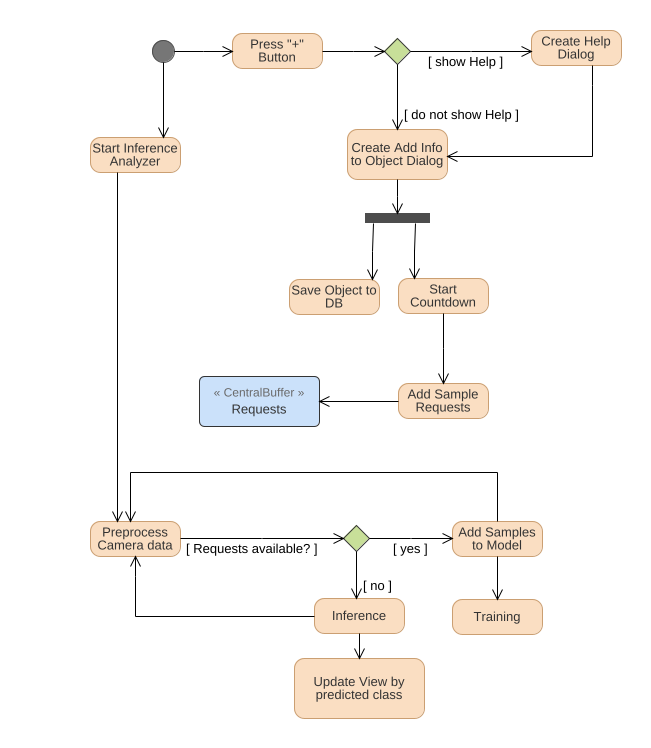
\includegraphics[height=0.6\textheight]{images/addobject-diagram.png}	\caption{UML-Aktivitätsdiagramm: Einlernen und Wiedererkennen von Objekten} Quelle: Eigene Darstellung
	\label{fig:activity-diagram-model}
\end{figure}
\subsection{Speichern und Laden von Parameterdateien}
Eine Parameterdatei bezeichnet die Parametrisierung des Modells, welche binär in einer Datei abgespeichert wird. Um Mehrdeutigkeit zu vermeiden wird die Bezeichnung \textit{model-parameters} mit einer möglichst zufällig generierten Zeichenfolge und dem Suffix \textit{.bin} konkateniert und eine leere Datei wird im Verzeichnis der Applikation erzeugt.\\
Die Transfer Learning \ac{api} stellt Methoden zum Speichern und Laden von Modell-Parametern zur Verfügung. Durch das Erzeugen eines Ein-/Ausgabestromes können die Dateien unter Angabe des absoluten Pfades der eben generierten leeren Datei zur Laufzeit der Applikation geladen beziehungsweise mit Binärdaten gefüllt werden.
\subsection{Anbindung des Latent-Replay Algorithmus}
Zu Beginn der Entwicklung der Applikation wurde lediglich auf Basis des Model-Personalization-Beispiels, welches von Tensorflow Lite zur Verfügung gestellt wird, die Funktionalität der Wiedererkennung von Objekten realisiert. Im Laufe der Testphase, wurde jedoch klar, dass das Phänomen des Katastrophalen Vergessens fatal für eine wiederverwendbare Applikation ist. Transfer Learning funktioniert, solange das Modell nicht geschlossen beziehungsweise neu gestartet wird. Bereits das Wechseln der Fragmente zur Laufzeit verursacht das Schließen des Transfer Learning Modells. Dies hat zur Folge, dass die Trainingsdaten aus der letzten Sitzung nicht mehr für das Modell zur Verfügung stehen.\\
Bereits in der Anfangsphase dieser Projektarbeit, wurde der Latent-Replay Algorithmus von Pellegrini et al. studiert, welcher eine Lösung zum Phänomen des Katastrophalen Vergessens vorstellt \cite{Pellegrini2019}. Aufgrund keiner vorhandenen Beispielimplementierung wurde dieser Ansatz jedoch verworfen.\\
Im Laufe der Implementierungsphase der Applikation dieser Projektarbeit publizierten Demosthenous et al. ein Paper mit zugehörigem offenen Quellcode, welcher die Einbindung des Latent-Replay Algorithmus unter Verwendung der Transfer Learning API massiv erleichtern konnte \cite{cl-vs-tl}. Auf Basis dieser Beispielimplementierung wurde der Algorithmus eingebunden. Lediglich wenige Änderungen waren hierfür notwendig.\\
Sobald der Analysierer Trainingsanfragen erhält, werden während dem Hinzufügen der Trainingsdaten zum zugrundeliegenden Modell, die Daten persistent in der Datenbank abgespeichert, um diese später beim Ausführen des Latent-Replay erneut einzulernen.\\
Methoden, in welchen die neuen Trainingsdaten an das Modell weitergegeben werden, werden durch eine Replay-Methode erweitert. Daraufhin werden die Trainingsdaten zusammen mit bereits vorhandenen Trainingsdaten zusammen trainiert und das Phänomen des Katastrophalen Vergessens kann gelöst werden.
\subsection{Belegen der Modellpositionen mit Objekten}
Das Anknüpfen der Objekte an die zur Verfügung stehenden Modellpositionen wird im Folgenden erklärt.\\
Jedes Deep Learning Modell hat am am Ende der Netzarchitektur eine vordefinierte Anzahl an Ausgabeknoten, welche für die endgültige Klassifizierung nach Prozessieren der Eingabedaten einen Wert zwischen 0 und 1 annimmt. Diese ausgegebene Zahl kann als Konfidenzwert, das heißt die Sicherheit mit welcher das Modell die Eingabedaten diesem Ausgabeknoten zuordnen kann, interpretiert werden.\\
Durch eine festdefinierte Anzahl an Ausgabeknoten, ergibt sich eine Einschränkung der gleichzeitig wiedererkennbaren Objekte, welches durch das Einführen von Objektordnern gelöst wird. Die Bezeichnung Objektordner ist gleichbedeutend mit der auch im Quellcode vorkommenden Bezeichnung Model und wurde gewählt, um den Nutzer mit technischen \ac{ml}-spezifischen Begriffen nicht zu überfordern.\\
Es ist demnach möglich Objekte in ein Objektordner in Höhe der Anzahl an verfügbaren Endknoten des Modells zu speichern. In der Modellübersicht, beziehungsweise der Ordnerübersicht, lässt sich die Parametrisierung des Modells durch Selektieren eines anderen bereits bestehenden Modells wechseln.\\
Bereits gespeicherte Objekte enthalten immer eine Referenz auf das Modell, welches die Bilddaten des Objektes trainiert hat.\\
Das Camera Fragment View Model hält eine Liste an verfügbaren Modellpositionen. Bei Erzeugung des Fragments wird diese Liste mit der Anzahl an Objekten, die das ausgewählte Modell referenzieren, abgeglichen. Sobald ein Objekt zu diesem Modell gehört und eine Modellposition zugewiesen bekommen hat, wird die entsprechende Position aus der Liste des Viewmodels entfernt.\\
Beim Hinzufügen von neuen Objekten wird die erste Position, die in der im View Model gespeicherten Liste vorkommt, zum Objekt hinzugefügt und persistent mit diesem abgespeichert. Falls die Liste leer ist, wird der Nutzer darüber informiert, dass der Objektordner, beziehungsweise das Modell, voll ist.
\subsection{Konfigurierbarkeit}
Die Konfigurierbarkeit der Applikation, soll mit einem zusätzlichen Fragment gewährleistet werden, dessen einzige Aufgabe es ist die Globale Konfiguration, beispielsweise realisiert durch Shared Preferences, für den Nutzer zugänglich zu machen durch Buttons, Schieberegler und andere graphischen Steuerelemente. Die Nutzung der Schnittstelle zur Globalen Applikationskonfiguration wird anschließend von den restlichen Komponenten bei Bedarf angebunden.
\subsection{Entwurf der graphischen Oberfläche}
Die graphische Oberfläche soll möglichst intuitiv und übersichtlich gestaltet werden.\\
Zur Navigation soll eine Navigationsleiste am unteren Bildschirmrand hinzugefügt werden und eine weitere aufklappbare Alternativleiste soll am linken oberen Bildschirmrand geöffnet werden können.\\
Aktions- und Steuerelemente sollen mit möglichst selbsterklärenden Icons besetzt werden. Um das \glqq Principle of Least Surprise\grqq\ zu gewährleisten, sollen Klicks auf Buttons meistens lediglich Dialoge erzeugen. In diesen Dialogen wird erneut erklärt, was die nächste Aktion zur Folge hat. Unter Anwendung der Globalen Konfiguration, soll eine Checkbox mit der Beschreibung \glqq Nicht mehr anzeigen\grqq\ das Erzeugen von Dialogen unterdrücken, um die Arbeit mit der Applikation für erfahrene Nutzer beschleunigen zu können.\\
Nachdem eine Aktion, wie beispielsweise das Hinzufügen oder Löschen von Objekten abgeschlossen ist, soll dies dem Nutzer mithilfe von sogenannten Toasts, die bei Android eine Art Notifier-Popup darstellen, mitgeteilt werden, um stets eine Rückmeldung des Systems gewährleisten zu können. Länger andauernde Operationen, wie beispielsweise dem Trainieren von Objekten, oder dem Aktualisieren des Latent-Replay-Puffers, soll mithilfe von Ladekreisen hervorgehoben werden, um dem Nutzer zu signalisieren, dass das System eine länger andauernde Operation durchführt. Da das Ende des Trainings durch das Entfernen des letzten Elementes in der Anfragewarteschlange gekennzeichnet ist, kann hierfür ein deterministischer Ladekreis verwendet werden, welcher dem Nutzer eine präzisere Angabe für die verbleibende Dauer des Prozesses zur Verfügung stellen kann.\\
Die Oberfläche der Applikation wird in deutsch und englisch verfügbar sein. Dies ist möglich durch das Verwenden von extern gespeicherten Zeichenketten in einer Datei im XML-Format, welche stets als Platzhalter in den Quelltext der Applikation eingebunden werden können. Je nach Systemsprache des Betriebssystems, auf welchem die Applikation ausgeführt wird, kann die Sprache dynamisch festgelegt werden. Falls eine andere nicht übersetzte Sprache als Systemsprache ausgewählt ist, wird standardmäßig die Datei, welche die englischen Zeichenketten beinhaltet, als Fallback-Lösung verwendet.\\
Ein Dunkelmodus wird nach einem ähnlichen Prinzip zur Verfügung gestellt. Durch das Auslagern von Farben und Stilen in dafür vorgesehene XML-Dateien, kann die Applikation das Farbschema der Oberfläche dynamisch ändern.\\
In Anhang \ref{appendix:gui} werden Screenshots von der Gestaltung der graphischen Oberfläche dargestellt.
\chapter{Implementierung}
\label{cha:implementierung}
In diesem Kapitel wird die konkrete Implementierung des in Kapitel
\ref{cha:Entwurf} entwickelten Lösungskonzepts beschrieben.\\
Hierbei wird auf die konkret verwendeten Entwicklungswerkzeuge und Implementierungsdetails der Applikation eingegangen.
\section{Entwicklungswerkzeuge}
Im Folgenden werden Werkzeuge, die die Entwicklung der Applikation vereinfachen, vorgestellt.
\subsection{Android Studio}
\textit{Android Studio} ist eine auf IntelliJ basierende Entwicklungsumgebung der Firma Jetbrains, die von der Open-Source Community und Google entwickelt wird. Es ist die offizielle Entwicklungsumgebung für Android-Apps \cite{android-studio-basics}.\\
Die Applikation wurde mithilfe von Android Studio implementiert, da es ein breites Spektrum an hilfreichen Werkzeugen zur Android-App-Entwicklung zur Verfügung stellt. Genutzt wurden vor allem ein integrierter Emulator, ein Datenbankuntersuchungswerkzeug und der integrierte Debugger. Zum Messen von kritischen Code-Abschnitten, wird ein Profiler zur Verfügung gestellt, der die Systemauslastung in Echtzeit misst.

\subsection{Gradle}
Mithilfe des Build-Tools \textit{Gradle} wird die lauffähige Applikation erzeugt. Gradle erleichtert die Kontrolle über die Abhängigkeit von Third-Party-Software. Zudem ist es möglich Konfigurationen, die vor dem Bauvorgang vorgenommen werden sollen, anzuwenden.\\
Tabelle \ref{tab:gradle-config}, zeigt die vorgenommenen Android-spezifischen Konfigurationsparameter, die für die Kompatibilität mit unterschiedlichen Endgeräten zuständig sind und deren in der Implementierung angegebene API Level.\\
\begin{table}[htbp]
	\centering
	\begin{tabular}{|l|p{1cm}|p{8.5cm}|}
		\hline
		\textbf{Parameter} & \textbf{API-Level} & \textbf{Beschreibung} \\ \hline
		\texttt{compileSdkVersion} & 30 & Kompiliert wird mit API Level 30. Diese Option hat lediglich Auswirkungen zur Kompilierzeit  \\ \hline
		\texttt{minSdkVersion} & 26 & Setzt die minimal zu verwendende Version vorraus. Geräte, die diese Version nicht installiert haben können demnach nicht verwendet werden. Aufgrund der Nutzung diverser API Level 26 Funktionen wurde die Version dementsprechend hochgesetzt \\ \hline
		\texttt{targetSdkVersion} & 30 & Gewährleistet Aufwärtskompatibilität bis in dieses API Level. Dieser Wert sollte höchstens so hoch wie der Wert von \texttt{compileSdkVersion}  \\ \hline
	\end{tabular}
	\caption{Kompatibilitätskonfiguration mit Gradle}
	\label{tab:gradle-config}
\end{table}Weitere wichtige Einstellungen, die in der \texttt{build.gradle}-Datei vorzunehmen waren, sind Optionen für das sogenannte Android Asset Packaging Tool (AAPT). Die einzelnen Bestandteile des zugrundliegenden Modells, die im \texttt{.tflite}-Format gespeichert sind, sollen nicht durch das Packaging-Tool komprimiert werden, da das korrekte Prozessieren der Daten dadurch nicht mehr möglich ist. Demnach muss die Option \texttt{noCompress "tflite"} in dem zugehörigen Block der Datei angegeben werden.\\ 
Standardmäßig wird von Tensorflow Lite am Ende der \texttt{build.gradle}-Datei eine Funktion hinzugefügt, welche aus dem Internet ein Modell herunterlädt und in das für die Transfer Learning Library auffindbare Verzeichnis im Projekt kopiert.\\
Da für die Applikation jedoch eine modifizierte Version der Modellarchitektur genutzt wird, welche zehn statt den von Tensorflow Lite standardmäßig festgelegten vier Endknoten beinhaltet, werden diese Zeilen auskommentiert.
\section{Implementierung der Kamerafunktionalität mit CameraX}
\textit{CameraX} ist eine sogenannte \textit{Jetpack support library} von Android. Diese Bibliotheken werden zur Verfügung gestellt, um Boilerplate-Code in der Kernlogik der Applikation vermeiden zu können. Zudem werden die Anwendung von \textit{best practices} und die Kompatibilität mit diversen Android Versionen unterstützt \cite{android:jetpack}.\\
Die CameraX-Bibliothek stellt eine einfach benutzbare \ac{api} zur Verfügung, die für die App, die in diesem Projekt entwickelt werden soll, eingesetzt wird \cite{android:camerax}. Die Anwendungsfälle, die hierbei erfüllt werden sind:
\begin{enumerate}
	\item Eine Vorschau der Kameradaten auf dem Display
	\item Bildanalyse-/prozessierung
	\item Bilderfassung
\end{enumerate}
Das Anzeigen der Kameradaten in Echtzeit entspricht dem ersten Punkt und wird dementsprechend mit diesem Teil der CameraX-\ac{api} implementiert.\\
Der in Kapitel \ref{cha:train-objects} erwähnte Bildanalysierer, der die Daten an den Trainings- bzw Inferenzprozess weiterleitet, wird durch den zweiten Punkt implementiert.\\
Um lediglich Bilder zu erfassen, die in im Rahmen der Fokusbox sind, wurde der dritte Punkt nicht genutzt. Die bereits korrekt zugeschnitteten Kameradaten wurden im Analysierer in Form einer Bitmap an die SQLite-Datenbankschnittstelle übergeben. Diese Bitmaps werden in Byte-Felder konvertiert und als \ac{blob} gespeichert. Das Konvertieren und Zurückkonvertieren in eine anzeigbare Bitmap wird direkt von der SQLite-Datenbankschnittstelle übernommen.
\subsection{Implementierung der konfigurierbaren Fokusbox}
Die Implementierung der in der Größe konfigurierbaren Fokusbox konnte durch das Erweitern der von Android zur Verfügung gestellten \texttt{ImageView}, welche das Anzeigen von Bildern und Grafiken auf der Benutzeroberfläche ermöglicht, realisiert werden.\\
Ein Objekt der \texttt{Paint}-Klasse wird erzeugt, welches unter anderem Informationen über die Größe und Farbe einer geometrischen Form enthält. Ein transparentes Quadrat wird hierbei in eine durchsichtige abdunkelnde Form geschnitten, welche der Größe des Bildschirms entspricht. Dies ist durch das Überschreiben der \texttt{onDraw}-Methode möglich, welche beim Zeichnen der graphischen Oberfläche aufgerufen wird. Die entworfene Form wird beim Erstellen des Kamerafragements als Overlay eingefügt und gibt dem Nutzer den Hinweis, welcher Bereich der Kamera für die Einlern- und Wiedererkennungsfunktionalität eingefangen wird.\\
Die Eckpunkte des Quadrats werden in den Shared Preferences indirekt festgelegt. Ein Schieberegler in der Einstellungsansicht ermöglicht es zwischen den drei Modi \textit{Klein}, \textit{Mittel} und \textit{Groß} zu wählen, welche lediglich einem \texttt{Double}-Wert zwischen $0$ und $1$ zugeordnet sind. Groß bedeutet hierbei, dass die Breite des Bildschirms komplett genutzt werden soll und die Höhe dementsprechend angepasst wird, um die Form eines Quadrats behalten zu können. Der Wert ist demnach auf $1.0$ festgelegt. Analog hierzu sind die Einstellungsmöglichkeiten \textit{Mittel} auf $0.75$ und \textit{Klein} auf $0.5$ festgelegt. Es ist bei Belieben demnach mit wenig Aufwand möglich diese Werte anzupassen oder weitere Größeneinstellungen hinzuzufügen.\\
Der Bildanalysierer führt demnach stets die Größenberechnung durch, um das Training beziehungsweise die Inferenz auf den Bereich des Bildschirms zu begrenzen, welcher innerhalb der Fokusbox liegt.

\section{Implementierung der Persistenzschnittstelle mit SQLite und Shared Preferences}
Zur strukturierten Speicherung der Entitätsklassen wird für die Implementierung der Persistenzschnittstelle der Zugriff auf eine SQLite Datenbank implementiert. SQLite ist die meistgenutzte Datenbank-Engine der Welt. Sie ist in allen mobilen Endgeräten installiert und überzeugt durch dessen Robustheit und Abwärtskompatibilität \cite{sqlite-documentation}. Die in Kapitel \ref{cha:design:entities} beschriebenen Entitätsklassen wurden wie in Quelltext 5.1 implementiert.\\ \\
\begin{minipage}{\linewidth}
\begin{lstlisting}[language=SQL, breaklines=true, caption={SQLite Statements zum Erstellen der Tabellen}]
CREATE TABLE object_table (
	object_ID INTEGER PRIMARY KEY AUTOINCREMENT,
	object_name TEXT UNIQUE NOT NULL,
	object_type TEXT,
	object_additional_data TEXT,
	object_created_at DATETIME DEFAULT CURRENT_TIMESTAMP,
	object_image BLOB,
	model_pos TEXT,
	model_id INTEGER NOT NULL,
	object_amount_samples INTEGER,\\
	FOREIGN KEY(model_id) REFERENCES model_table(model_ID));

CREATE TABLE model_table (
	model_ID INTEGER PRIMARY KEY AUTOINCREMENT,
	model_name TEXT UNIQUE NOT NULL,
	model_path TEXT,
	is_frozen INTEGER DEFAULT 0);

CREATE TABLE replay_buffer_images (
	buffer_id INTEGER PRIMARY KEY AUTOINCREMENT,
	class TEXT NOT NULL, 
	sample_blob BLOB NOT NULL,
	model_id INTEGER NOT NULL);
	
CREATE TABLE training_samples (
	sample_id INTEGER PRIMARY KEY AUTOINCREMENT,
	class TEXT NOT NULL,
	sample BLOB NOT NULL,
	sample_timestamp TIMESTAMP DEFAULT CURRENT_TIMESTAMP,
	model_id INTEGER NOT NULL);
\end{lstlisting}
\label{lst:sql-statements}
\end{minipage}
Die Daten werden in sogenannte \texttt{Cursor}-Objekte gespeichert und können spaltenweise iteriert werden mit der \texttt{moveToNext()}-Methode. Die Datenbank-Helferklasse \texttt{SQLiteDatabase} stellt zudem verschiedene Methoden zum Einfügen, Aktualisieren und Löschen von Reihen in der Datenbank zur Verfügung. Dies erleichtert den Umgang mit dem persistenten Speichern von Daten, da es dadurch möglich ist SQL-Anfragen in einer einzelnen Zeile Quelltext zu formulieren.\\
Da das Speichern von Booleschen Werten nicht von SQLite unterstützt wird, wird die \texttt{isFrozen}-Spalte als Integer-Wert gespeichert. Der Wert 0 entspricht hierbei \texttt{false} und 1 entspricht \texttt{true}.\\
Das Datum wird als Unix-Zeitstempel, welcher die vergangenen Sekunden seit dem 1. Januar 1970 um 0 Uhr zählt, gespeichert. Dies vereinfacht unter anderem das chronologische Sortieren der Daten. Mithilfe des \texttt{SimpleDateFormat}-Pakets kann dieses Datum in ein lesbares Format gebracht und auf der graphischen Benutzeroberfläche angezeigt werden.\\
Um das Abspeichern von Objekten und Modellen mit gleichen Namen zu vermeiden, wird \texttt{model\_name} und \texttt{object\_name} mit dem Schlüsselwort \texttt{UNIQUE} deklariert, um direkt auf Datenbankebene entscheiden zu können, dass ein Objekt beziehungweise ein Modell mit diesem Namen bereits vorhanden ist.\\
Die in Kapitel \ref{cha:communication-components} erklärte Kommunikation der Komponenten wird vor allem durch Shared Preferences gestützt. Diese ermöglichen es auch nach Schließen der App, Daten zu halten und abzurufen, die für den Ablauf der Prozesse wichtig sind.\\
Der \texttt{SharedPrefsHelper} implementiert die \texttt{GlobalConfig}-Schnittstelle.\\
Die Shared Preferences können durch einfache Befehle, wie in Quelltext 5.2 dargestellt, gesetzt und abgefragt werden. Der Schlüssel des gespeicherten Key-Value-Paares wird beim Setzen der Shared Preference initialisiert, falls er noch nicht vorhanden ist und aktualisiert, falls ein Key mit dem angegebenen Namen bereits existiert.\\
Zudem können beim Abfragen Standardwerte gesetzt werden, die zurückgegeben werden, falls der Wert für diesen Schlüssel noch nicht gesetzt worden ist. Dies kann beispielsweise beim ersten Start nach Installation der Applikation, oder durch das Zurücksetzen der Applikation durch das Betätigen der jeweiligen Option in den internen App-Einstellungen, der Fall sein.

\begin{minipage}{\linewidth}
	\begin{lstlisting}[language=Java, breaklines=true, caption={Auschnitt aus SharedPrefsHelper}]
// ...
@Override
public int getAmountSamples() {
	return prefs.getInt("key_num_samples"), 50);
}

// ...

@Override
public boolean getHelpShowing() {
	return prefs.getBoolean("key_show_help", true);
}

@Override
public void setHelpShowing(boolean show) {
	SharedPreferences.Editor editor = prefs.edit();
	editor.putBoolean("key_show_help", show);
	editor.apply();
}

// ...

@Override
public String getCurrentModelID() {
	return prefs.getString("key_current_model", null);
}

@Override
public void setCurrentModelID(String id) {
	SharedPreferences.Editor editor = prefs.edit();
	editor.putString("key_current_model", id);
	editor.apply();
}
// ...
	\end{lstlisting}
\end{minipage}
\label{lst:shared-prefs}

%---
\chapter{Tests}
\label{cha:tests}
Im Rahmen der zu entwickelnden Applikation sind diverse Tests durchzuführen, um eine qualitativ hochwertige und fehlerfreie Software ausliefern zu können.\\
Zum Einen wurden Unit-Tests zum Testen der einzelnen Methoden erstellt. Diese sind hilfreich für das Verändern oder Refactoring einzelner Methoden, da die Logik des Quellcodes auf diese Weise stets überprüft werden kann. Zum anderen wurde ein Akzeptanztest für das Testen des korrekten Zusammenspiels aller Komponenten in einer natürlichen Testumgebung erstellt, um mögliche Fehler oder UI/UX-spezifische Unklarheiten vor Beginn der Auslieferung der Applikation beheben zu können.
\section{Unit-Tests}
Für die Implementierung der zu schreibenden Tests werden die Test Frameworks \texttt{JUnit} und AndroidX-Testbibliotheken standardmäßig von Android Studio bei Erstellung eines Projektes eingebunden und demnach auch für das Testen der zu entwickelnden Applikation genutzt. Für die Assertions der Tests wird für eine bessere Lesbarkeit die von Google zur Verfügung gestellte Bibliothek \texttt{Truth} verwendet.\\
Für das Erstellen von instrumentierten Unit-Tests, welche auf einem Android-Emulator ausgeführt werden, werden AndroidX Tests in einer Ordnerstruktur angelegt, welche der Struktur des Hauptprojektes entspricht. Diese instrumentierten Unit-Tests sind notwendig für das Testen von Methoden, welche Android-spezifische Abhängigkeiten enthalten, wie beispielsweise \textit{Activities} oder \textit{Contexts} und nicht lokal auf dem Entwicklungsrechner ausführbar sind. Alle anderen Tests werden mit \texttt{JUnit} geschrieben und sind demnach schneller ausführbar, da sie in der lokalen Java Virtual Machine (JVM) ausgeführt werden können und demnach die Verwendung eines Emulators nicht notwendig ist.\\
Aus Zeitgründen konnte kein extensives Testing durchgeführt werden für die meisten Komponenten. Die Implementierung der Datenbankhelferklasse wurde jedoch auf den gesamten Wertebereich getestet, um eine möglichst hohe Testabdeckung erzielen zu können.\\

\section{Akzeptanztest}
Die durch Unit-Tests getestete Applikation, wurde als Beta-Test im Rahmen einer Feldstudie getestet. Mithilfe eines Fragebogens, der von den Testern ausgefüllt wurde, konnten Ergebnisse und Eindrücke gesammelt werden, die für die weitere Entwicklung der Applikation von Bedeutung sein können. Außerdem konnten noch einige Bugs identifiziert und gelöst werden.\\
Bei den Testern handelt es sich um Frauen und Männer, im Alter zwischen 18 und 50 Jahren mit keiner Erfahrung im Fachgebiet der Informatik. Demnach konnten Ergebnisse von Laien verschiedener Altersgruppen erfasst werden, welche unterschiedliche Hardware zur Ausführung der Applikation genutzt haben.\\
Die Ergebnisse sind in Anhang \ref{appendix:beta-test} zu finden. Ein überwiegend positiver Eindruck über die Applikation konnte festgestellt werden. Lediglich die Einfachheit der Benutzung wurde aufgrund von diversen User-Interface-Designfehlern kritisiert, welche größtenteils behoben werden konnten.\\
Demnach wurden aus den Ergebnissen diverse Änderungen an der Oberfläche vorgenommen. Der Begriff \glqq Model\grqq, sorgte bei den Testern für Verwirrung. Demnach wurde er zu \glqq Objektordner\grqq\ auf der graphischen Oberfläche abgeändert, um den technischen Hintergrund zu verbergen. Die Implementierung führt jedoch weiterhin den Begriff Model. Durch das Verwenden von externen String-Ressourcen, konnte das Umbenennen in kurzer Zeit realisiert werden. \\
Der ausklappbare Text oberhalb der Kamera-Ansicht, welcher den Namen und die weiteren gespeicherten Daten des Objekts beinhaltet, wurde hervorgehobener gestaltet, um das Blickfeld des Nutzers an den oberen Bildschirmrand zu lenken. Zudem wurde die Schriftfarbe des \glqq Training\grqq-Schriftzugs, der sich ebenfalls an der oberen Leiste befindet, gewechselt, um den Nutzer auf das laufende Training besser aufmerksam machen zu können.\\
Die oben genannten Probleme, die für die Tester entstanden sind, könnten auch durch die Verwendung eines \texttt{OnBoardingSupportFragment} gelöst werden. Dieses Fragment ermöglicht es diverse Hilfeelemente beim ersten Start der Applikation anzeigen zu lassen. Mithilfe des \texttt{HelpFragments}, zu welchem man stets navigieren kann, erhält der Nutzer ebenfalls eine textuelle Anleitung für die Nutzung der Applikation.\\
Diverse Darstellungsbugs, wie sich überlappende Elemente der graphischen Oberfläche, oder \textit{TextViews}, die nicht den gesamten Text dargestellt haben, konnten ebenfalls durch die Beta-Tests gefunden, reproduziert und behoben werden.
%---
\chapter{Zusammenfassung und Ausblick}
\label{cha:zusammenfassung}

\section{Erreichte Ergebnisse}
\label{sec:ergebnisse}

Die Zusammenfassung dient dazu, die wesentlichen Ergebnisse des 
Praktikums und vor allem die entwickelte Problemlösung und den 
erreichten Fortschritt darzustellen. (Sie haben Ihr Ziel erreicht und 
dies nachgewiesen).

\section{Ausblick}
\label{sec:ausblick}

Im Ausblick werden Ideen für die Weiterentwicklung der erstellten Lösung 
aufgezeigt. Der Ausblick sollte daher zeigen, dass die Ergebnisse der 
Arbeit nicht nur für die in der Arbeit identifizierten Problemstellungen 
verwendbar sind, sondern darüber hinaus erweitert sowie auf andere 
Probleme übertragen werden können.

\subsection{Erweiterbarkeit der Ergebnisse}
\label{sub:erweiterbarkeit}

Hier kann man was über die Erweiterbarkeit der Ergebnisse sagen.

\subsection{Übertragbarkeit der Ergebnisse}
\label{sub:uebertragbarkeit}

Und hier etwas über deren Übertragbarkeit.

\chapter{Fazit}

%-----------------------------------------------------------------------
\appendix

%---
\printbibliography[heading=bibintoc]

%---
\chapter{Beschreibung der Anwendungsfälle}
\label{appendix:use-cases}

\begin{table}[htbp]
	\centering
	\begin{tabular}{|l|p{80mm}|}
		\hline
		\textbf{Nummer} & \textbf{AF-M1} \\ \hline
		\textbf{Anwendungsfall} & \textbf{Modell hinzufügen} \\ \hline
		\textbf{Beschreibung} & Beliebig viele neue Modelle sollen hinzufügt werden können \\ \hline
		\textbf{Akteur} & Nutzer \\ \hline
		\textbf{Auslöser} & Der Nutzer betätigt den "+"-Button in der Modellübersicht oder startet die Applikation zum ersten Mal  \\ \hline
		\textbf{Vorbedingung} & Der Nutzer befindete sich in der Modellübersicht oder hat bisher noch kein Modell hinzugefügt  \\ \hline	
		\textbf{Nachbedingung/Ziel} & Ein Modell zu welchem weitere Objekte hinzugefügt werden können, wurde gespeichert \\ \hline
		\textbf{Nachbedingung im Sonderfall} & Das Modell wurde nicht gespeichert und der Nutzer wird darüber durch eine Fehlermeldung informiert \\ \hline
		\textbf{Standardablauf} & 1. Dialogfenster öffnet sich \\ 
		& 2. Nutzer gibt Namen für Modell ein\\
		& 3. Neues Modell wird gespeichert und Nutzer wird darüber informiert\\ \hline
		\textbf{Sonderfälle} & 2a. Ein Modell mit dem  Namen existiert bereits \\ & $\rightarrow$ Der Nutzer wird darüber mit einer Fehlermeldung informiert\\
		& 3a. Das Modell konnte nicht gespeichert werden \\ & $\rightarrow$ Der Nutzer wird darüber mit einer Fehlermeldung informiert \\ \hline
		
	\end{tabular}
	\caption{Anwendungsfall M1: Modell hinzufügen}
	\label{tab:use-case-add-model}
\end{table}

\begin{table}[htbp]
	\centering
	\begin{tabular}{|l|p{80mm}|}
		\hline
		\textbf{Nummer} & \textbf{AF-M2} \\ \hline
		\textbf{Anwendungsfall} & \textbf{Modell wechseln} \\ \hline
		\textbf{Beschreibung} & Das ausgewählte Modell soll gewechselt werden können mit einem anderen bestehenden Modell \\ \hline
		\textbf{Akteur} & Nutzer \\ \hline
		\textbf{Auslöser} & Der Nutzer befindet sich in der Modellübersicht und betätigt den Radiobutton, der sich links neben dem Modellnamen befindet  \\ \hline
		\textbf{Vorbedingung} & Es sind bereits mehrere Modelle hinzugefügt worden \\ \hline	
		\textbf{Nachbedingung/Ziel} & Es wurde ein anderes Modell ausgewählt \\ \hline
		\textbf{Nachbedingung im Sonderfall} & Das Modell wurde nicht gewechselt \\ \hline
		\textbf{Standardablauf} & 1. Nutzer betätigt den Radiobutton neben dem Namen des Modells \\
		& 2. Der Radiobutton wird als selektiert markiert und das Modell wurde gewechselt \\ \hline
		\textbf{Sonderfälle} & 2a. Das Modell konnte nichte selektiert werden \\ & $\rightarrow$ Keine Sonderbehandlung dieses Falles notwendig \\ \hline
		
	\end{tabular}
	\caption{Anwendungsfall M2: Modell wechseln}
	\label{tab:use-case-change-model}
\end{table}

\begin{table}[htbp]
	\centering
	\begin{tabular}{|l|p{80mm}|}
		\hline
		\textbf{Nummer} & \textbf{AF-M3} \\ \hline
		\textbf{Anwendungsfall} & \textbf{Gespeicherte Objekte im Modell betrachten} \\ \hline
		\textbf{Beschreibung} & Alle im Modell abgespeicherten Objekte sollen besichtigt werden können \\ \hline
		\textbf{Akteur} & Nutzer \\ \hline
		\textbf{Auslöser} & Der Nutzer betätigt den Button welcher sich rechts neben dem Modellnamen befindet  \\ \hline
		\textbf{Vorbedingung} & Der Nutzer befindet sich in der Modellübersicht und ein Modell wurde bereits abgespeichert \\ \hline	
		\textbf{Nachbedingung/Ziel} & Ein Dialogfenster, welches zum Modell alle gespeicherten Objekte anzeigt wurde geöffnet \\ \hline
		\textbf{Nachbedingung im Sonderfall} & Es wurden noch keine Objekte für das Modell abgespeichert und ein Hilfetext befindet sich im geöffneten Dialog \\ \hline
		\textbf{Standardablauf} & 1. Nutzer betätigt den Button, welcher sich rechts neben dem Modell befindet, dessen Objekte betrachtet werden sollen \\
		& 2. Ein Dialogfenster öffnet sich, welches eine Listenansicht aller zum Modell gespeicherten Objekte enthält \\ \hline
		\textbf{Sonderfälle} & 2a. Es öffnet sich keine Listenansicht, da noch kein Objekt für das jeweilige Modell abgespeichert wurde \\ & $\rightarrow$ Der Nutzer wird über das Fehlen von Objekten durch einen Text in der Mitte des Dialogfensters informiert \\ \hline
		
	\end{tabular}
	\caption{Anwendungsfall M3: Gespeicherte Objekte im Modell anschauen}
	\label{tab:use-case-view-saved-objects}
\end{table}

\begin{table}[htbp]
	\centering
	\begin{tabular}{|l|p{80mm}|}
		\hline
		\textbf{Nummer} & \textbf{AF-M4} \\ \hline
		\textbf{Anwendungsfall} & \textbf{Alle Modelle betrachten} \\ \hline
		\textbf{Beschreibung} & Alle abgespeicherten Modelle sollen mitsamt wichtiger Informationen besichtigt werden können \\ \hline
		\textbf{Akteur} & Nutzer \\ \hline
		\textbf{Auslöser} & Das Modell soll eingefroren werden. Das bedeutet, dass der Latent-Replay Algorithmus bei Ende der Trainingssitzung nicht mehr ausgeführt wird.  \\ \hline
		\textbf{Vorbedingung} & Es wurden bereits ein oder mehrere Modelle gespeichert \\ \hline	
		\textbf{Nachbedingung/Ziel} &  Der Nutzer befindet sich in der Modellübersicht, in welcher die gespeicherten Modelle betrachtet werden können\\ \hline
		\textbf{Nachbedingung im Sonderfall} & Die Modellübersicht enthält einen Text welcher daraufhinweist, dass bisher noch kein Modell gespeichert wurde, um einen leeren Bildschirm zu vermeiden \\ \hline
		\textbf{Standardablauf} & 1. Der Nutzer betätigt den Button in der Navigationsleiste der zur Modellübersicht führt \\
		& 2. Der Nutzer befindet sich in der Modellübersicht, welche eine Listenansicht der gespeicherten Objekte anzeigt, mitsamt der Anzahl bereits gespeicherter Objekte \\ \hline
		\textbf{Sonderfälle} & 2a. Es öffnet sich keine Listenansicht, da noch kein Modell abgespeichert wurde. \\ & $\rightarrow$ Der Nutzer wird über das Fehlen von Modellen durch einen Text in der Mitte des Bildschirms informiert \\ \hline
		
	\end{tabular}
	\caption{Anwendungsfall M4: Alle Modelle betrachten}
	\label{tab:use-case-view-models}
\end{table}

\begin{table}[htbp]
	\centering
	\begin{tabular}{|l|p{80mm}|}
		\hline
		\textbf{Nummer} & \textbf{AF-M5} \\ \hline
		\textbf{Anwendungsfall} & \textbf{Modell einfrieren} \\ \hline
		\textbf{Beschreibung} & Das Modell soll eingefroren werden. Das bedeutet, dass der Latent-Replay Algorithmus bei Ende der Trainingssitzung nicht mehr ausgeführt wird. Diese Kontrolle dem Nutzer zu übergeben, bietet den Vorteil, dass der Nutzer nicht durch langes Warten bei Ende der Trainingssitzung aufgrund des rechenintensiven Latent-Replay Algorithmus überrascht wird und die Möglichkeit hat das Modell fertigzustellen und nicht weiter zu trainieren. \\ \hline
		\textbf{Akteur} & Nutzer \\ \hline
		\textbf{Auslöser} & Der Nutzer verlässt die Trainingssitzung durch Wechseln der App mithilfe der Navigationsleiste  \\ \hline
		\textbf{Vorbedingung} & Nutzer hat in dieser Trainingssitzung ein neues Objekt hinzugefügt \\ \hline	
		\textbf{Nachbedingung/Ziel} & Das Modell wurde eingefroren \\ \hline
		\textbf{Nachbedingung im Sonderfall} & Das Modell wurde nicht eingefroren und der Latent-Replay Algorithmus wurde ausgeführt, um das Phänomen des Katastrophalen Vergessens in der nächsten Trainingssitzung zu verhindern \\ \hline
		\textbf{Standardablauf} & 1. Nutzer wechselt den Kameratab durch Betätigen eines Reiters in der Navigationsleiste \\
		& 2. Dialogfenster öffnet sich, welches den Nutzer darüber informiert, dass er nun die Möglichkeit hat sein Modell einzufrieren und welche Folgen dies hat. \\
		& 3. Nutzer betätigt den Button, der das Modell einfriert \\
		& 4. Es wird kein aufwendiger Algorithmus bei Ende der Trainingssitzung durchgeführt \\ \hline
		\textbf{Sonderfälle} & 3a. Nutzer betätigt den Button, der das Modell auf eine nächste Trainingssitzung vorbereitet \\
		& 3b. Latent-Replay Algorithmus wird ausgeführt und der Nutzer wird durch einen Ladekreis dazu angehalten bis zum Ende der Ausführung mit der Fortsetzung der Nutzung der Applikation zu warten \\ \hline
		
	\end{tabular}
	\caption{Anwendungsfall M5: Modell einfrieren}
	\label{tab:use-case-freeze-model}
\end{table}


\begin{table}[htbp]
	\centering
	\begin{tabular}{|l|p{80mm}|}
		\hline
		\textbf{Nummer} & \textbf{AF-O1} \\ \hline
		\textbf{Anwendungsfall} & \textbf{Objekt hinzufügen} \\ \hline
		\textbf{Beschreibung} & Objekte sollen hinzugefügt werden können \\ \hline
		\textbf{Akteur} & Nutzer \\ \hline
		\textbf{Auslöser} & Der Nutzer betätigt den \glqq+\grqq-Button der sich in der Mitte der Navigationsleiste befindet  \\ \hline
		\textbf{Vorbedingung} & Der Nutzer befindet sich in der Kamera-Ansicht und hat bereits ein Modell hinzugefügt \\ \hline	
		\textbf{Nachbedingung/Ziel} & Ein Objekt konnte erfolgreich zum derzeitig ausgewählten Modell hinzugefügt werden und kann wiedererkannt werden \\ \hline
		\textbf{Nachbedingung im Sonderfall} & Das Objekt wurde nicht abgespeichert \\ \hline
		\textbf{Standardablauf} & 1. Nutzer befindet sich in der Kamera-Ansicht und betätigt den \glqq+\grqq-Button in der Mitte der Navigationsleiste \\ 
		& 2. Ein Dialogfenster öffnet sich, welches den Nutzer darüber informiert was nun zu tun ist. Er hat nun die Möglichkeit diese Meldung nicht mehr anzuzeigen durch das Klicken des Hakens neben dem Text \glqq Nicht mehr anzeigen\grqq \\
		& 3. Nutzer betätigt den \glqq Fortfahren\grqq-Button \\
		& 4. Ein Dialogfenster öffnet sich, welches den Nutzer dazu auffordert dem Objekt Informationen hinzuzufügen \\
		& 5. Nutzer gibt korrekte Daten ein und startet Training durch das Betätigen des \glqq Training\grqq-Buttons\\ 
		& 6. Das Dialogfenster schließt sich und ein Countdown beginnt, welcher das bevorstehende Einlesen ankündigt \\
		& 7. Das Training wurde gestartet und der Nutzer wird darüber durch Ändern des Textes am rechten oberen Bildschirmran in \glqq Training\grqq\ und einem deterministischen Ladekreis im rechten oberen Bildschirmrand informiert \\
		& 8. Das Training  wurde abgeschlossen und der Text am rechten oberen Bildschildrand ändert sich wieder zu \glqq Erkennen\grqq \\ \hline
		\textbf{Sonderfälle} & 1a. Der Nutzer befindet sich in der Kamera-Ansicht \\ & $\rightarrow$ Die Ansicht wird durch Betätigen des Buttons zur Kamera-Ansicht gewechselt \\
		& 5a. Der Name des Objekts ist bereits vergeben \\ & $\rightarrow$ Der Nutzer wird darüber informiert und das Training wird noch nicht gestartet \\ 
		& 7a. Der Nutzer verlässt frühzeit die Kamera-Ansicht, obwohl das Training noch nicht abgeschlossen ist \\ 
		& 7b. Alle Objektplätze des ausgewählten Modells sind bereits belegt \\ & $\rightarrow$ Der Nutzer wird über diesen Fehler informiert. Das Training wird abgebrochen und das Objekt gelöscht \\ \hline
		
	\end{tabular}
	\caption{Anwendungsfall O1: Objekt hinzufügen}
	\label{tab:use-case-add-object}
\end{table}

\begin{table}[htbp]
	\centering
	\begin{tabular}{|l|p{80mm}|}
		\hline
		\textbf{Nummer} & \textbf{AF-O2} \\ \hline
		\textbf{Anwendungsfall} & \textbf{Objekte wiedererkennen} \\ \hline
		\textbf{Beschreibung} & Bereits eingespeicherte Objekte sollen durch Nutzung der Kamera wiedererkannt werden, wenn sich das Objekt innerhalb der Fokusbox befindet \\ \hline
		\textbf{Akteur} & Nutzer \\ \hline
		\textbf{Auslöser} & Der Nutzer kann das wiederzuerkennende Objekt in der Kamera-Ansicht sehen, da die Kamera des Mobilgeräts auf dieses Objekt ausgerichtet ist  \\ \hline
		\textbf{Vorbedingung} & Das Objekt wurde bereits eingespeichert und der Nutzer befindet sich in der Kamera-Ansicht \\ \hline	
		\textbf{Nachbedingung/Ziel} & Das Objekt wird korrekt erkannt und die Informationen über das Objekt werden am oberen Bildschirmrand angezeigt \\ \hline
		\textbf{Nachbedingung im Sonderfall} & Das Objekt wurde nicht erkannt \\ \hline
		\textbf{Standardablauf} & 1. Nutzer zeigt mit der Kamera auf das Objekt \\ 
		& 2. Das Objekt wird erkannt und eingespeicherte Informationen über das Objekt werden für den Nutzer angezeigt\\ \hline
		\textbf{Sonderfälle} & 2a. Das Objekt wurde nicht erkannt \\ & $\rightarrow$ Nutzer hat die Möglichkeit weitere Eindrücke über das Objekt zu sammeln, oder gewisse Einstellungen an der Applikation vorzunehmen, um das Problem selbstständig beheben zu können\\ \hline
		
	\end{tabular}
	\caption{Anwendungsfall O2: Objekt wiedererkennen}
	\label{tab:use-case-recognize-objects}
\end{table}

\begin{table}[htbp]
	\centering
	\begin{tabular}{|l|p{80mm}|}
		\hline
		\textbf{Nummer} & \textbf{AF-O3} \\ \hline
		\textbf{Anwendungsfall} & \textbf{Objekt bearbeiten} \\ \hline
		\textbf{Beschreibung} & Die Attribute, die für das Objekt gespeichert wurden, sollen geändert werden können \\ \hline
		\textbf{Akteur} & Nutzer \\ \hline
		\textbf{Auslöser} & Der Nutzer betätigt den \glqq Bearbeiten\grqq-Button in der Objektübersicht \\ \hline
		\textbf{Vorbedingung} & Der Nutzer befindet sich in der Objektübersicht und es sind bereits Objekte eingspeichert \\ \hline	
		\textbf{Nachbedingung/Ziel} & Der Nutzer kann durch das Öffnen eines Dialogfensters die bereits gespeicherten Informationen eines Objektes abändern \\ \hline
		\textbf{Nachbedingung im Sonderfall} & Es sind keine Objekte eingespeichert und der Nutzer hat dementsprechend keine Möglichkeit ein Objekt abzuändern \\ \hline
		\textbf{Standardablauf} & 1. Der Nutzer betätigt den \glqq Bearbeiten\grqq-Button in der Objektübersicht \\
		& 2. Ein Dialogfenster öffnet sich, welches den Nutzer dazu auffordert das Objekt zu bearbeiten \\
		& 3. Der Nutzer bearbeitet die Informationen korrekt \\
		& 4. Der Nutzer betätigt den \glqq Bestätigen\grqq -Button und kehrt zur Objektübersicht zurück \\ \hline
		\textbf{Sonderfälle} & 3a. Der Nutzer gibt einen neuen Objektnamen ein, der bereits existiert \\ & $\rightarrow$ Nutzer wird darauf hingewiesen und die Änderungen werden nicht gespeichert \\
		& 4a. Der Nutzer betätigt den Abbrechen Button \\ & $\rightarrow$ Die Änderungen werden nicht gespeichert \\ \hline
		
	\end{tabular}
	\caption{Anwendungsfall O3: Objekt bearbeiten}
	\label{tab:use-case-edit-object}	
\end{table}

\begin{table}[htbp]
	\centering
	\begin{tabular}{|l|p{80mm}|}
		\hline
		\textbf{Nummer} & \textbf{AF-O4} \\ \hline
		\textbf{Anwendungsfall} & \textbf{Weitere Trainingsdaten für Objekt erfassen} \\ \hline
		\textbf{Beschreibung} & Es sollen zu einem bestehenden Objekt weitere Trainingsdaten erfasst werden, um die Erkennungsgenauigkeit für das gewählte Objekt erhöhen zu können\\ \hline
		\textbf{Akteur} & Nutzer \\ \hline
		\textbf{Auslöser} & Der Nutzer betätigt den \glqq + \grqq-Button der sich unterhalb des Vorschaubildes des Objekts in der Listenansicht befindet  \\ \hline
		\textbf{Vorbedingung} & Es wurde bereits ein Objekt abgespeichert und der Nutzer befindet sich in der Objektübersicht\\ \hline	
		\textbf{Nachbedingung/Ziel} & Es wurde eine neue Trainingssitzung gestartet und dem Objekt wurde weitere Trainingsdaten hinzugefügt \\ \hline
		\textbf{Nachbedingung im Sonderfall} & Das Training wurde nicht gestarte\\ \hline
		\textbf{Standardablauf} & 1. Nutzer betätigt den \glqq +\grqq-Button \\
		& 2. Die Applikation wechselt in die Kamera-Ansicht und das Training wird nach Ablauf des Countdowns gestartet \\ \hline
		\textbf{Sonderfälle} & 2a. Das Training konnte nicht gestartet werden \\ & $\rightarrow$ Der Nutzer wird darüber mit einer Fehlermeldung informiert \\ \hline
		
	\end{tabular}
	\caption{Anwendungsfall O4: Weitere Trainingsdaten für Objekt erfassen}
	\label{tab:use-case-add-further-samples}	
\end{table}

\begin{table}[htbp]
	\centering
	\begin{tabular}{|l|p{80mm}|}
		\hline
		\textbf{Nummer} & \textbf{AF-O5} \\ \hline
		\textbf{Anwendungsfall} & \textbf{Objekt löschen} \\ \hline
		\textbf{Beschreibung} & Ein Objekt soll gelöscht werden können, sodass dieses nicht mehr von der Applikation erkannt wird \\ \hline
		\textbf{Akteur} & Nutzer \\ \hline
		\textbf{Auslöser} & Der Nutzer betätigt den \glqq Löschen\grqq-Button   \\ \hline
		\textbf{Vorbedingung} & Der Nutzer befindet sich in der Objektübersicht und hat bereits ein Objekt eingespeichert  \\ \hline	
		\textbf{Nachbedingung/Ziel} & Das zu löschende Objekt wurde erfolgreich entfernt \\ \hline
		\textbf{Nachbedingung im Sonderfall} & Das zu löschende Objekt wurde nicht erfolgreich entfernt \\ \hline
		\textbf{Standardablauf} & 1. Der Nutzer betätigt den \glqq Löschen\grqq-Button \\ 
		& 2. Ein Dialogfenster öffnet sich, welches den Nutzer fragt, ob er sich sicher sei das Objekt zu löschen \\
		& 3. Der Nutzer bestätigt seine Sicherheit durch Betätigen des Buttons und das Objekt wird gelöscht \\ \hline
		\textbf{Sonderfälle} & 3a. Der Nutzer betätigt den \glqq Abbrechen\grqq-Button\\ & $\rightarrow$ Das Dialogfenster wird geschlossen und das Objekt wird nicht gelöscht \\ \hline
		
	\end{tabular}
	\caption{Anwendungsfall O5: Objekt löschen}
	\label{tab:use-case-delete-object}
\end{table}

\begin{table}[htbp]
	\centering
	\begin{tabular}{|l|p{80mm}|}
		\hline
		\textbf{Nummer} & \textbf{AF-O6} \\ \hline
		\textbf{Anwendungsfall} & \textbf{Alle Objekte betrachten} \\ \hline
		\textbf{Beschreibung} & Alle eingespeicherten Objekte sollen mitsamt aller Attribute des Objektes betrachtet werden können \\ \hline
		\textbf{Akteur} & Nutzer \\ \hline
		\textbf{Auslöser} & Der Nutzer wechselt in die Objektübersicht  \\ \hline
		\textbf{Vorbedingung} & Der Nutzer bereits Objekte eingespeichert \\ \hline	
		\textbf{Nachbedingung/Ziel} & Der Nutzer kann nun eine Listenansicht über alle abgespeicherten Objekte betrachten \\ \hline
		\textbf{Nachbedingung im Sonderfall} & Es wurden noch keine Objekte abgespeichert. Dementsprechend wurde keine Listenansicht erzeugt \\ \hline
		\textbf{Standardablauf} & 1. Nutzer wechselt durch Betätigen des jeweiligen Buttons in der Navigationsleiste in die Objektübersicht \\
		& 2. Nutzer betrachtet eine Liste, welche alle Objekte mit den zugehörig abgespeicherten Daten beinhaltet \\ \hline
		\textbf{Sonderfälle} & 2a. Es wurde noch kein Objekt abgespeichert \\ & $\rightarrow$ Es wird in der Mitte des Bildschirm ein Informationstext angezeigt, um eine komplett leere Ansicht zu vermeiden \\ \hline
		
	\end{tabular}
	\caption{Anwendungsfall O6: Alle Objekte betrachten}
	\label{tab:use-case-view-objects}
\end{table}

\begin{table}[htbp]
	\centering
	\begin{tabular}{|l|p{80mm}|}
		\hline
		\textbf{Nummer} & \textbf{AF-E1} \\ \hline
		\textbf{Anwendungsfall} & \textbf{Einstellen der Anzahl der hinzuzufügenden Daten pro Training} \\ \hline
		\textbf{Beschreibung} & Die Anzahl der Trainingsdaten die pro Objekttraining erfasst werden, soll konfigurierbar sein, um Kontrolle über die Dauer und die Genauigkeit der Erkennung zu erhalten \\ \hline
		\textbf{Akteur} & Nutzer \\ \hline
		\textbf{Auslöser} & Der Nutzer betätigt den jeweiligen Schieberegler in den App-Einstellungen \\ \hline
		\textbf{Vorbedingung} & Der Nutzer befindet sich in den App-Einstellungen \\ \hline	
		\textbf{Nachbedingung/Ziel} & Die Anzahl der hinzuzufügenden Daten pro Training wurde auf den neuen Wert angepasst \\ \hline
		\textbf{Nachbedingung im Sonderfall} & Änderung konnte nicht vollzogen werden \\ \hline
		\textbf{Standardablauf} & 1. Der Nutzer stellt den Schieberegler auf einen neuen Wert \\ 
		& 2. Die Anzahl der Trainingsdaten pro Objekttraining wird angepasst \\ \hline
		\textbf{Sonderfälle} & 2a. Anzahl der Trainingsdaten pro Objekttraining kann nicht angepasst werden \\ & $\rightarrow$ Der Nutzer wird darüber durch eine Fehlermeldung informiert \\ \hline
		
	\end{tabular}
	\caption{Anwendungsfall E1: Einstellen der Anzahl der hinzuzufügenden Daten pro Training}
	\label{tab:use-case-set-samples}
\end{table}

\begin{table}[htbp]
	\centering
	\begin{tabular}{|l|p{80mm}|}
		\hline
		\textbf{Nummer} & \textbf{AF-E2} \\ \hline
		\textbf{Anwendungsfall} & \textbf{Einstellen der Dauer des Countdowns vor dem Training} \\ \hline
		\textbf{Beschreibung} & Der unmittelbar vor dem Training laufende Countdown, soll konfigurierbar sein, um unnötige Wartezeiten, oder notwendige Zeiten für die korrekte Ausrichtung der Kamera zu ermöglichen \\ \hline
		\textbf{Akteur} & Nutzer \\ \hline
		\textbf{Auslöser} & Der Nutzer betätigt den jeweiligen Schieberegler in den App-Einstellungen \\ \hline
		\textbf{Vorbedingung} & Der Nutzer befindet sich in den App-Einstellungen \\ \hline	
		\textbf{Nachbedingung/Ziel} & Die Länge des Countdowns wurde auf den neuen Wert gesetzt \\ \hline
		\textbf{Nachbedingung im Sonderfall} & Die Länge des Countdowns konnte nicht auf den neuen Wert gesetzt werden \\ \hline
		\textbf{Standardablauf} & 1. Der Nutzer stellt den Schieberegler auf einen neuen Wert \\ 
		& 2. Die Länge des Countdowns wird angepasst \\ \hline
		\textbf{Sonderfälle} & 2a. Die Länge des Countdowns konnte nicht angepasst werden \\ & $\rightarrow$ Der Nutzer wird darüber durch eine Fehlermeldung informiert \\ \hline
		
	\end{tabular}
	\caption{Anwendungsfall E2: Einstellen der Dauer des Countdowns vor dem Training}
	\label{tab:use-case-set-countdown}
\end{table}

\begin{table}[htbp]
	\centering
	\begin{tabular}{|l|p{80mm}|}
		\hline\\
		\textbf{Nummer} & \textbf{AF-E3} \\ \hline
		\textbf{Anwendungsfall} & \textbf{Einstellen der Auflösung der hinzuzufügenden Trainingsdaten} \\ \hline
		\textbf{Beschreibung} & Die Größe der Fokusbox im Kamerahauptbildschirm soll konfigurierbar sein, um nahe beziehungs Objekte in der Ferne zu erfassen, ohne zu viel Hintergrund einzufangen \\ \hline
		\textbf{Akteur} & Nutzer \\ \hline
		\textbf{Auslöser} & Der Nutzer betätigt den jeweiligen Schieberegler in den App-Einstellungen \\ \hline
		\textbf{Vorbedingung} & Der Nutzer befindet sich in den App-Einstellungen \\ \hline	
		\textbf{Nachbedingung/Ziel} & Die Auflösung der hinzuzufügenden Trainingsdaten wird angepasst \\ \hline
		\textbf{Nachbedingung im Sonderfall} & Die Auflösung der hinzuzufügenden Trainingsdaten konnte nicht angepasst werden \\ \hline
		\textbf{Standardablauf} & 1. Der Nutzer stellt den Schieberegler auf einen neuen Wert \\
		& 2. Die Auflösung der hinzuzufügenden Trainingsdaten wird angepasst \\ \hline
		\textbf{Sonderfälle} & 2a. Die Auflösung der hinzuzufügenden Trainingsdaten konnte nicht angepasst werden \\ & $\rightarrow$ Der Nutzer wird darüber durch eine Fehlermeldung informiert \\ \hline
		
	\end{tabular}
	\caption{Anwendungsfall E3: Einstellen der Auflösung der hinzuzufügenden Trainingsdaten}
	\label{tab:use-case-set-resolution}
\end{table}

\begin{table}[htbp]
	\centering
	\begin{tabular}{|l|p{80mm}|}
		\hline
		\textbf{Nummer} & \textbf{AF-E4} \\ \hline
		\textbf{Anwendungsfall} & \textbf{Einstellen des Konfidenzschwellwerts bei Inferenz} \\ \hline
		\textbf{Beschreibung} & Der Konfidenzschwellwert soll konfigurierbar sein. Dies bedeutet, dass ein Objekt erst im Overlay angezeigt wird, wenn das Modell mit einer bestimmen Erkennungssicherheit (Konfidenz) das Objekt richtig erkannt hat \\ \hline
		\textbf{Akteur} & Nutzer \\ \hline
		\textbf{Auslöser} & Der Nutzer betätigt den jeweiligen Schieberegler in den App-Einstellungen \\ \hline
		\textbf{Vorbedingung} & Der Nutzer befindet sich in den App-Einstellungen \\ \hline	
		\textbf{Nachbedingung/Ziel} & Der Konfidenzschwellwert wurde auf den neuen Wert gesetzt \\ \hline
		\textbf{Nachbedingung im Sonderfall} & Der Konfidenzschwellwert konnte nicht auf den neuen Wert gesetzt werden \\ \hline
		\textbf{Standardablauf} & 1. Der Nutzer stellt den Schieberegler auf einen neuen Wert \\ 
		& 2. Der Konfidenzschwellwert wird angepasst \\ \hline
		\textbf{Sonderfälle} & 2a. Der Konfidenzschwellwert wird nicht angepasst \\ 
		& $\rightarrow$ Der Nutzer wird darüber durch eine Fehlermeldung informiert \\ \hline
		
	\end{tabular}
	\caption{Anwendungsfall E4: Einstellen des Konfidenzschwellwerts bei Inferenz}
	\label{tab:use-case-set-conf-thres}
\end{table}

\begin{table}[htbp]
	\centering
	\begin{tabular}{|l|p{80mm}|}
		\hline
		\textbf{Nummer} & \textbf{AF-E5} \\ \hline
		\textbf{Anwendungsfall} & \textbf{Applikation zurücksetzen} \\ \hline
		\textbf{Beschreibung} & Alle persistent gespeicherten Daten sollen zurückgesetzt werden können, um eine Alternative zur Neuinstallation der Applikation zu schaffen\\ \hline
		\textbf{Akteur} & Nutzer \\ \hline
		\textbf{Auslöser} & Der Nutzer betätigt das Feld in den App-Einstellungen, welches für das Zurücksetzen der Applikation zuständig ist \\ \hline
		\textbf{Vorbedingung} & Der Nutzer befindet sich in den App-Einstellungen\\ \hline
		\textbf{Nachbedingung/Ziel} & Alle Modelle, Objekte und sonstige Konfigurationen wurden auf Werkseinstellungen zurückgesetzt \\ \hline
		\textbf{Nachbedingung im Sonderfall} & Das Zurücksetzen war nicht erfolgreich \\ \hline
		\textbf{Standardablauf} & 1. Der Nutzer betätigt das Feld \\
		& 2. Ein Dialogfenster erscheint, welches den Nutzer darauf hinweist, dass das Zurücksetzen der Applikation nicht rückgängig gemacht werden kann und dass alle eingespeicherten Daten gelöscht werden \\ 
		& 3. Der Nutzer bestätigt das Zurücksetzen \\
		& 4. Die Applikation wird zurückgesetzt und neu gestartet \\ \hline
		\textbf{Sonderfälle} & 3a. Der Nutzer betätigt den \glqq Abbrechen \grqq-Button und das Dialogfenster schließt sich. Der Vorgang wird abgebrochen \\
		& 4a. Die Applikation konnte nicht zurückgesetzt werden \\ & $\rightarrow$ Der Nutzer wird darüber durch eine Fehlermeldung informiert und der Vorgang wird abgebrochen \\ \hline
		
	\end{tabular}
	\caption{Anwendungsfall E5: Applikation zurücksetzen}
	\label{tab:use-case-reset}
\end{table}

%---
\chapter{Umfrageergebnisse Beta-Test}
\label{appendix:beta-test}
Die Darstellung der Ergebnisse des Betatests wurden mithilfe von Google Forms erstellt.
\begin{figure}[hptb]
	\centering
	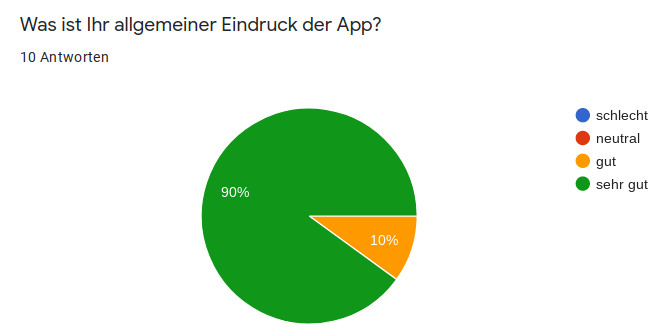
\includegraphics[height=0.3\textheight]{images/umfrage-allgemeiner-eindruck.png}
	\caption{Frage 1: Allgemeiner Eindruck}
	\label{fig:beta:allgemein}
\end{figure}

\begin{figure}[hptb]
	\centering
	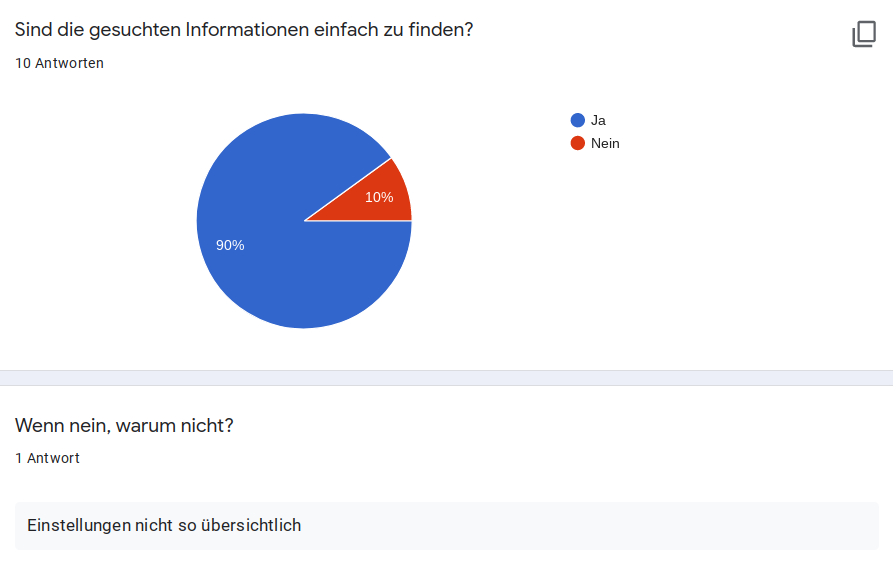
\includegraphics[height=0.5\textheight]{images/umfrage-einfach-zu-finden.png}
	\caption{Frage 2: Leichte Auffindbarkeit der Informationen}
	\label{fig:beta:einfach-zu-finden}
\end{figure}

\begin{figure}[hptb]
	\centering
	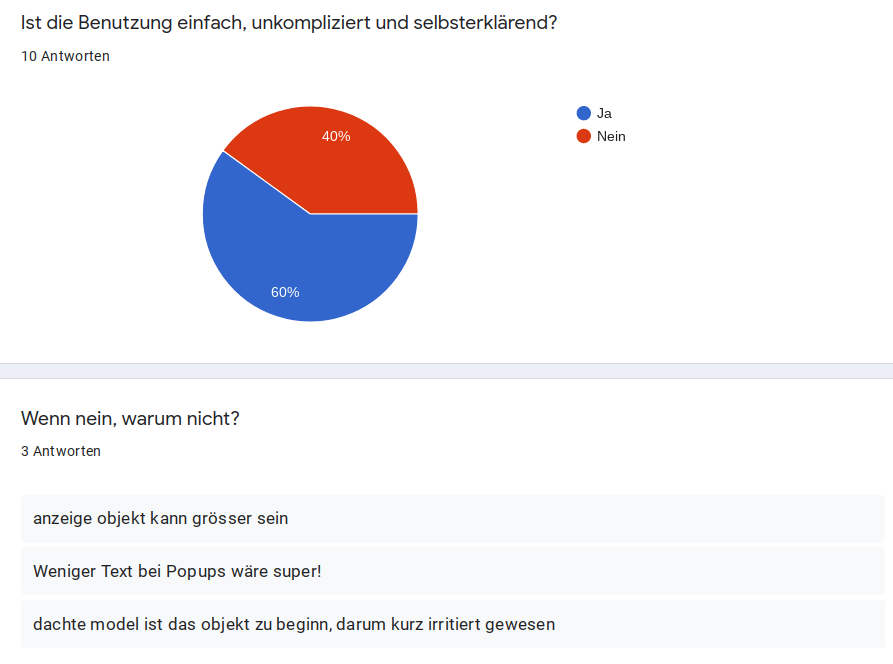
\includegraphics[height=0.5\textheight]{images/umfrage-selbsterklaerend.png}
	\caption{Frage 3: Intuitivität der Applikation}
	\label{fig:beta:selbsterklaerend}
\end{figure}

\begin{figure}[hptb]
	\centering
	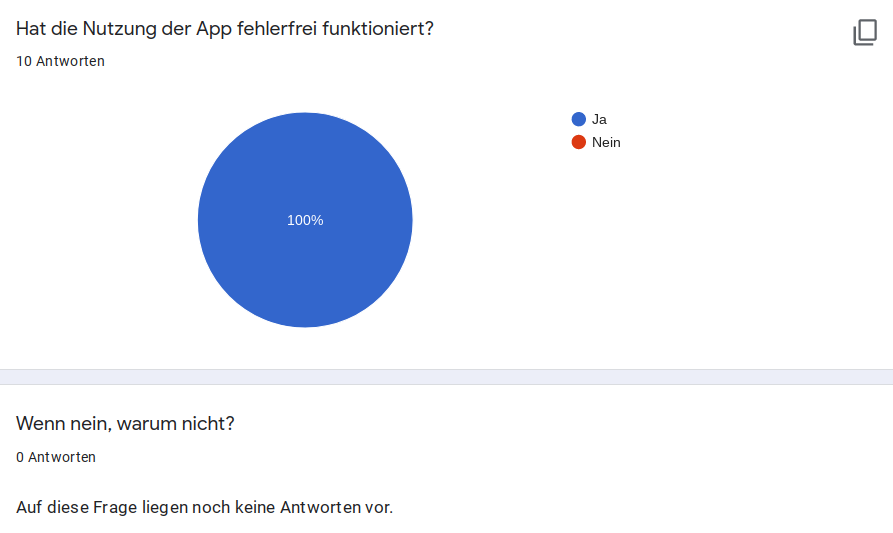
\includegraphics[height=0.4\textheight]{images/umfrage-fehlerfrei-funktioniert.png}
	\caption{Frage 4: Fehlerfreie Benutzung}
	\label{fig:beta:nobugs}
\end{figure}

\begin{figure}[hptb]
	\centering
	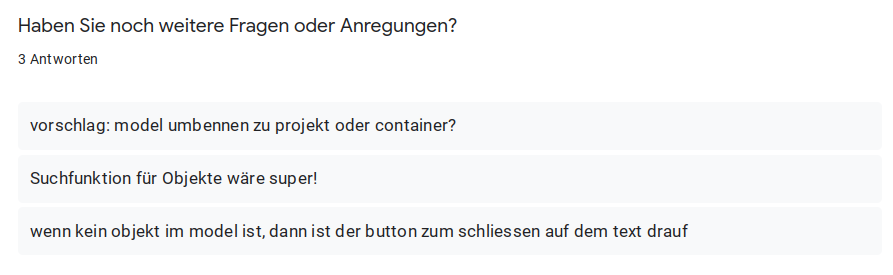
\includegraphics[height=0.25\textheight]{images/umfrage-further-questions.png}
	\caption{Frage 5: Weitere Anregungen oder Fragen}
	\label{fig:beta:further}
\end{figure}

\chapter{Screenshots der graphischen Benutzeroberfläche}
\label{appendix:gui}
\begin{figure}[hptb]
	\centering
	
\includegraphics[height=0.6\textheight]{images/screenshots/start-screen.png}
	\caption{Screenshot: Startbildschirm}
	\label{fig:screenshot:start}
\end{figure}
\begin{figure}[hptb]
	\centering
	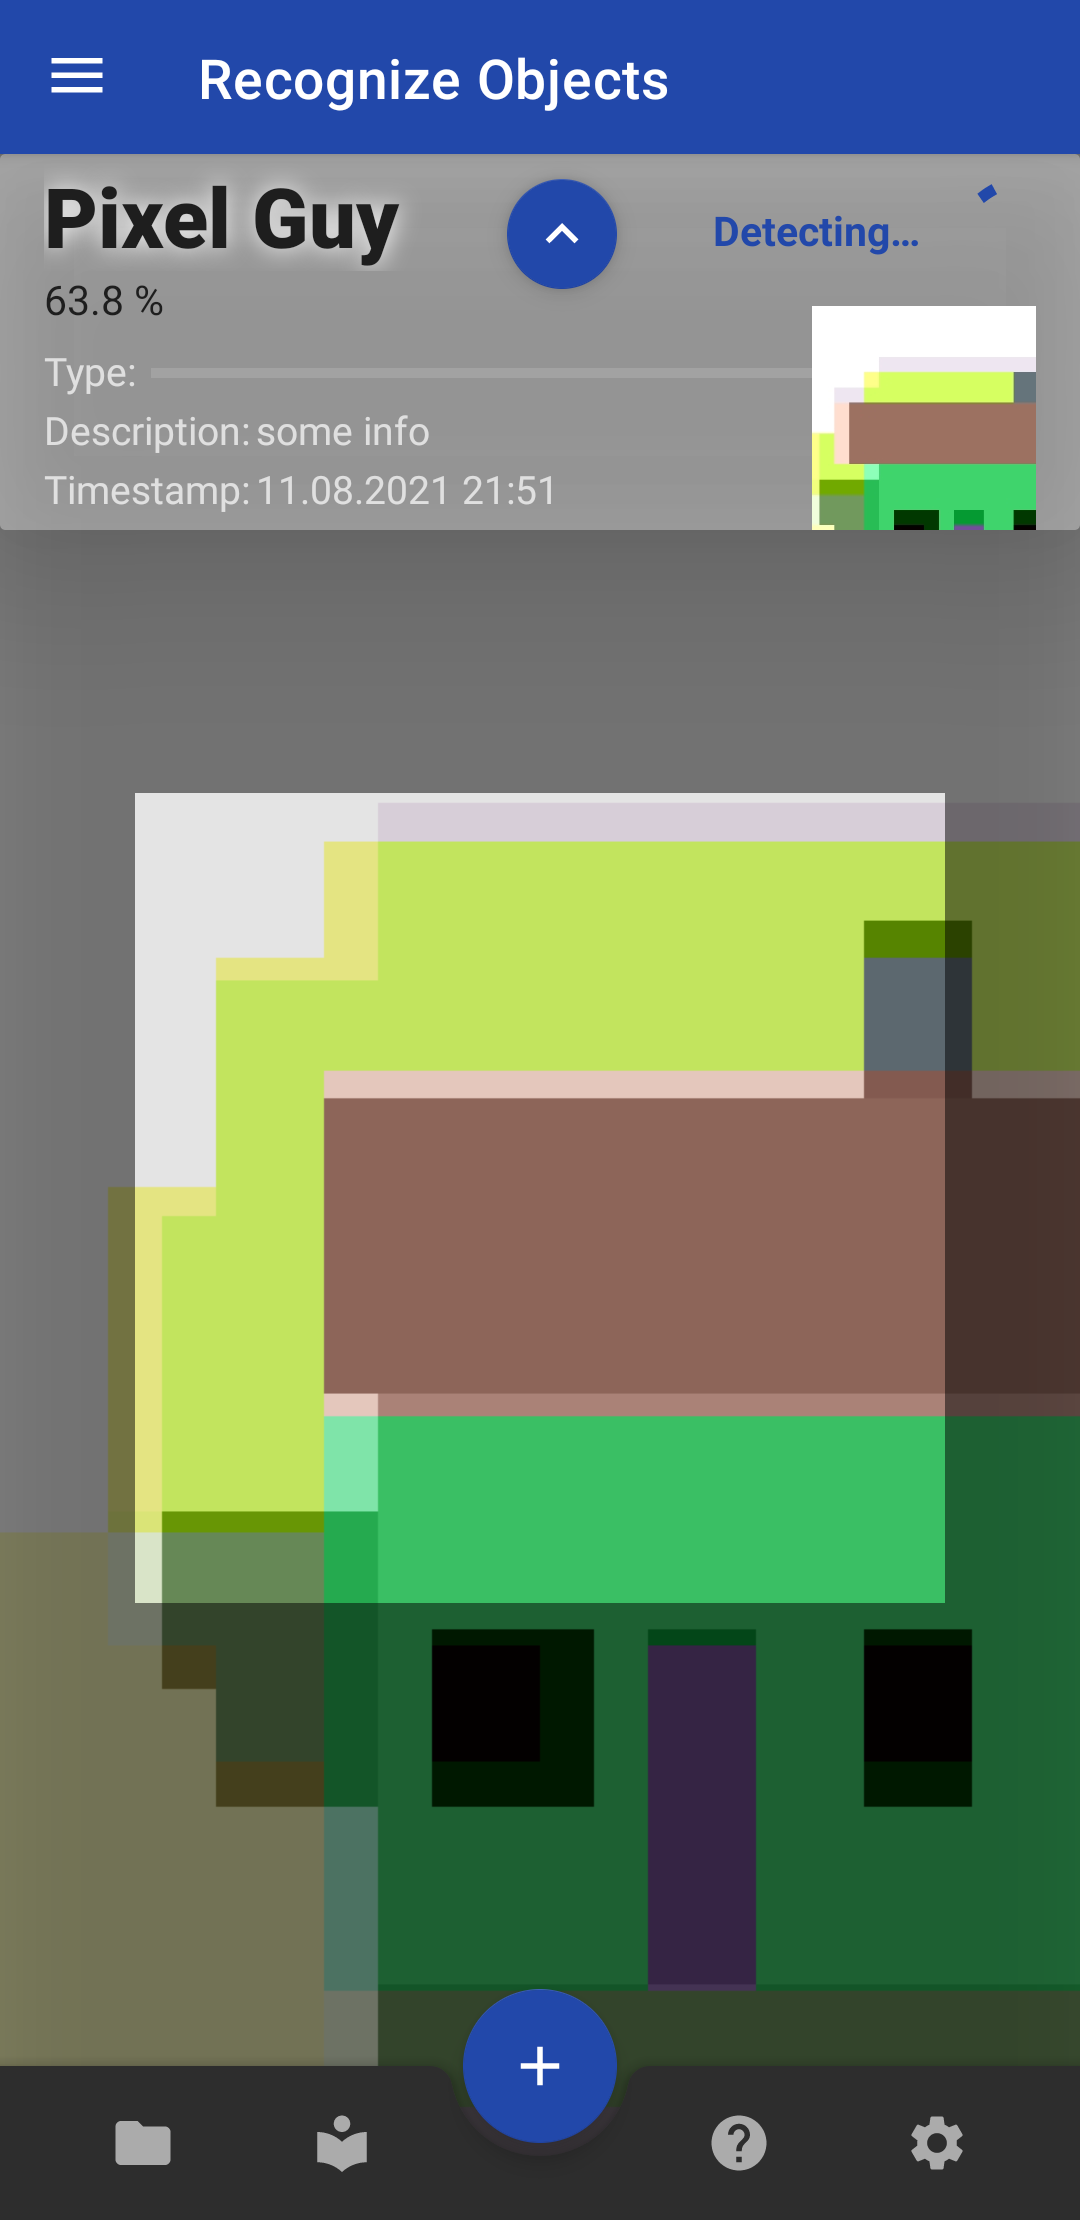
\includegraphics[height=0.6\textheight]{images/screenshots/detecting.png}
	\caption{Screenshot: Erkennen von Objekten}
	\label{fig:screenshot:detecting}
\end{figure}

\begin{figure}[hptb]
	\centering
	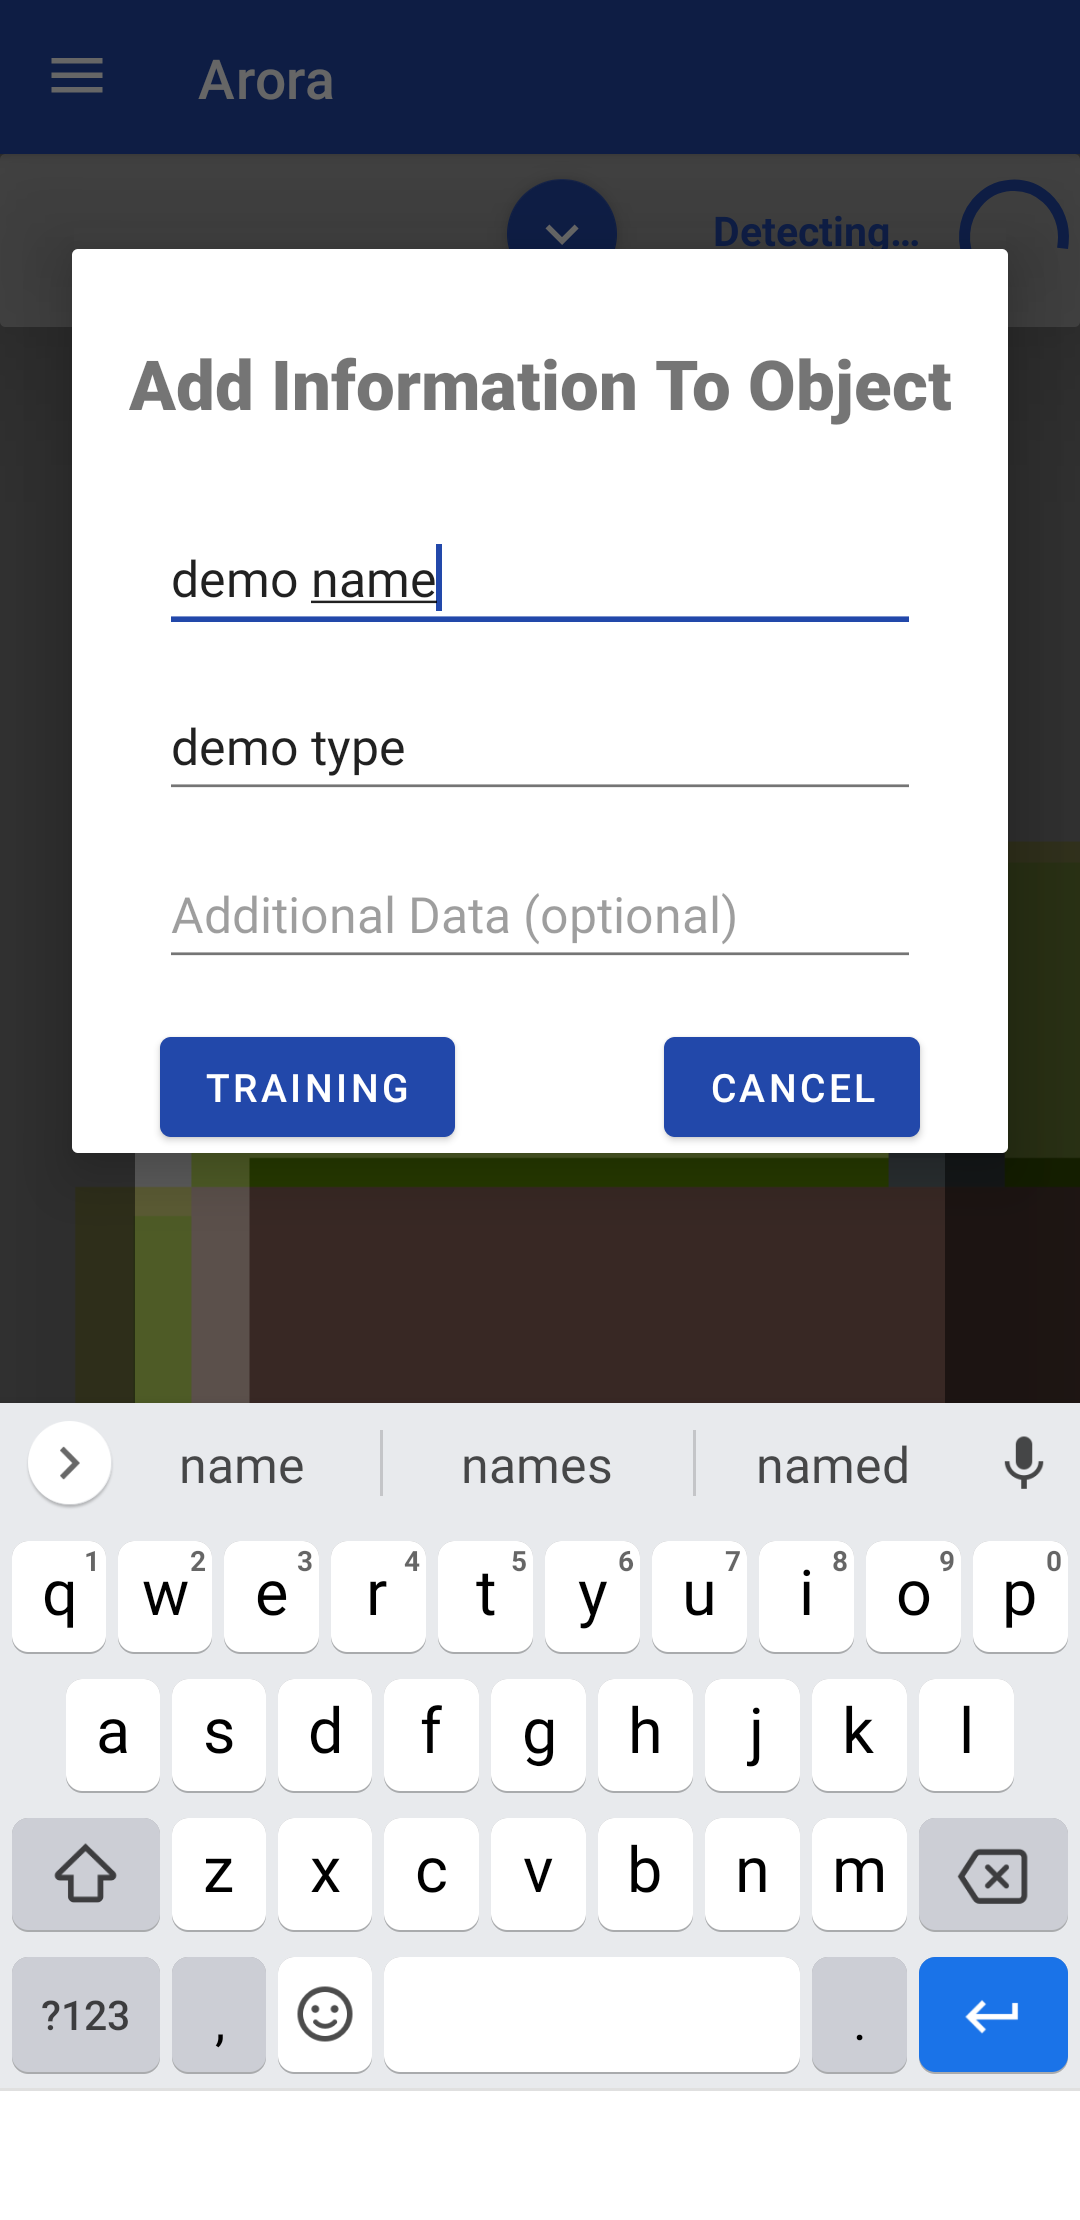
\includegraphics[height=0.6\textheight]{images/screenshots/add-info.png}
	\caption{Screenshot: Hinzufügen von Objektinformationen}
	\label{fig:screenshot:add-info}
\end{figure}

\begin{figure}[hptb]
	\centering
	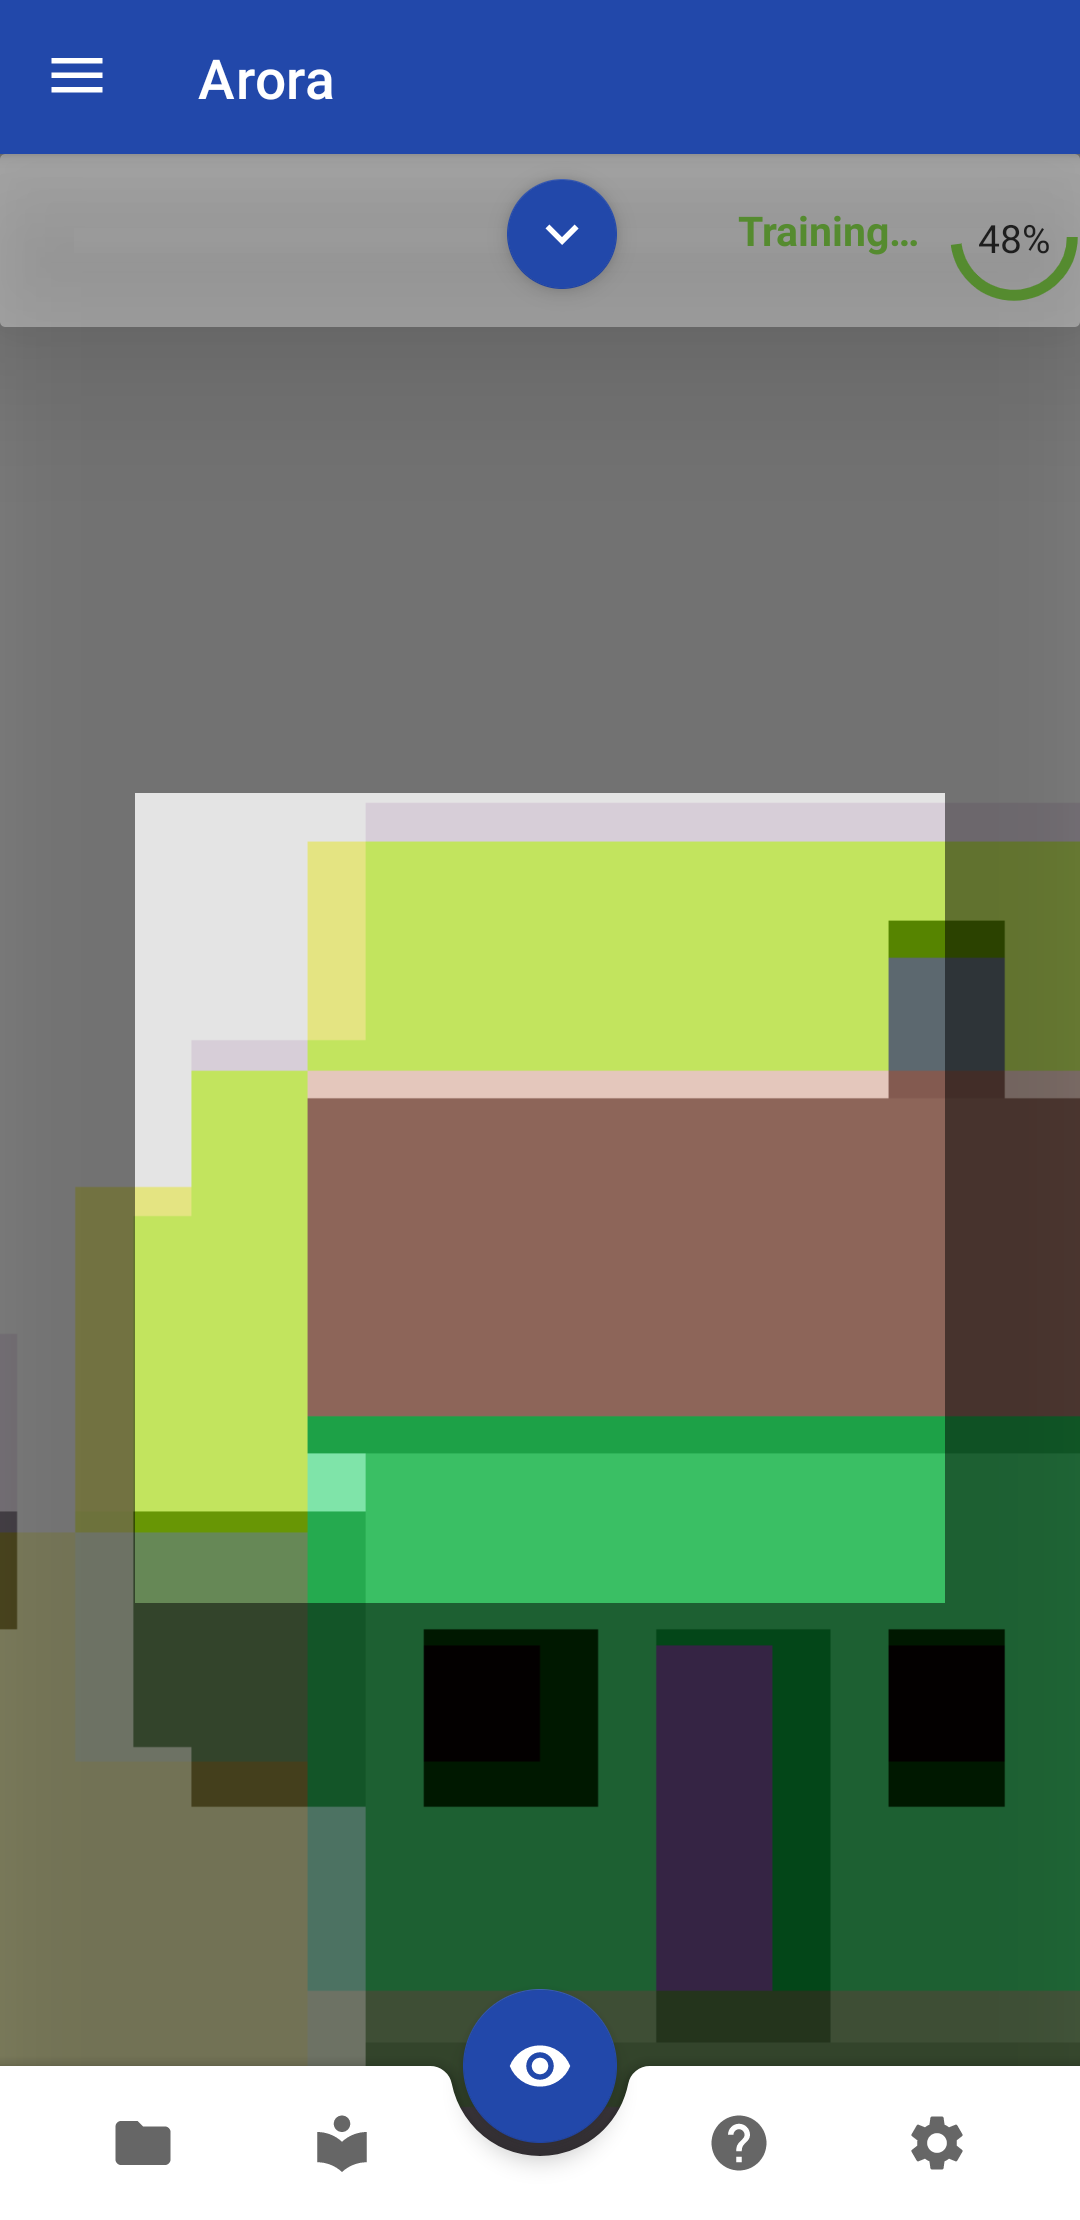
\includegraphics[height=0.6\textheight]{images/screenshots/training.png}
	\caption{Screenshot: Einlernen von Objekten}
	\label{fig:screenshot:training}
\end{figure}

\begin{figure}[hptb]
	\centering
	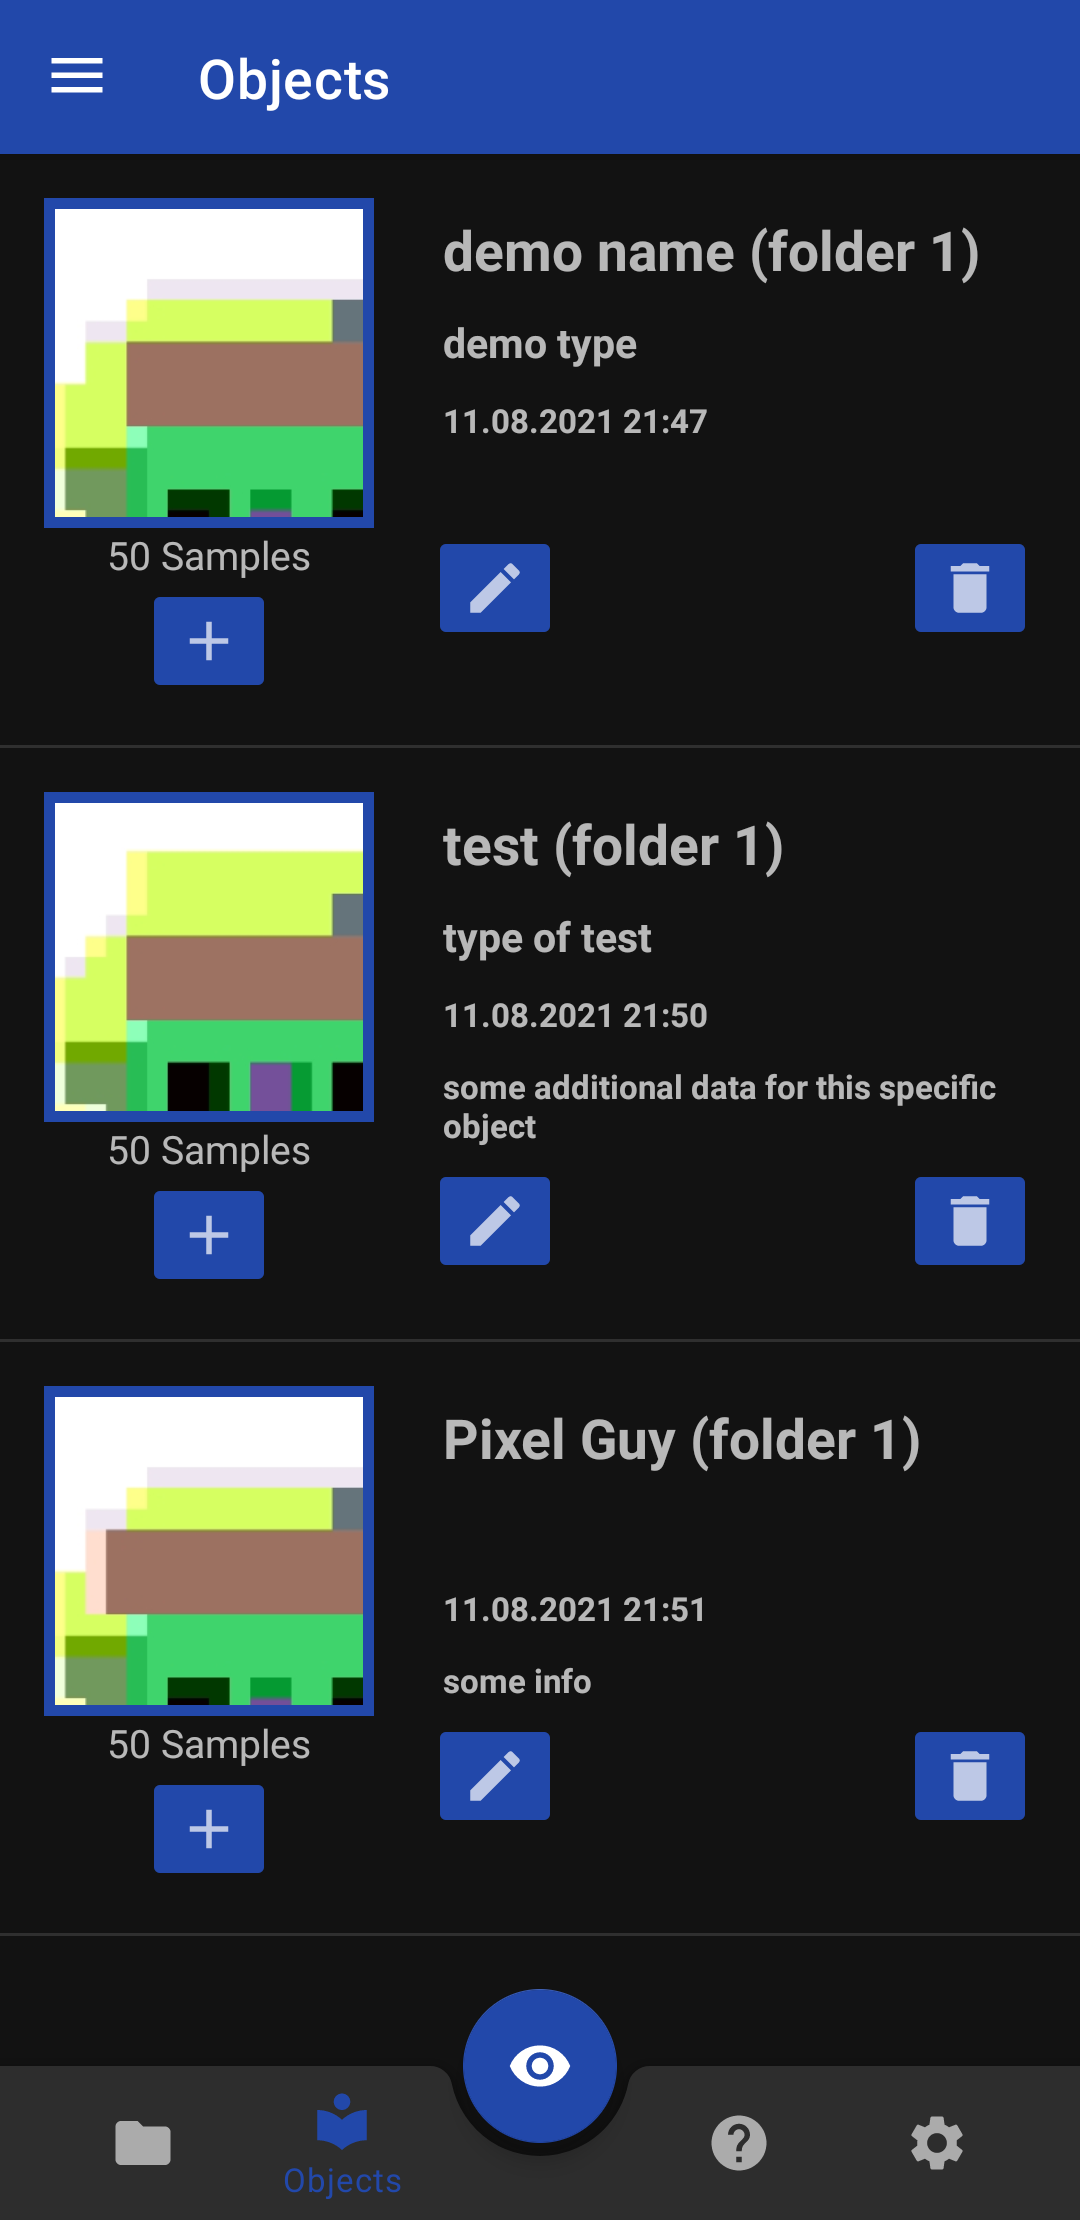
\includegraphics[height=0.6\textheight]{images/screenshots/object-overview.png}
	\caption{Screenshot: Objektübersicht}
	\label{fig:screenshot:obj-overview}
\end{figure}

\begin{figure}[hptb]
	\centering
	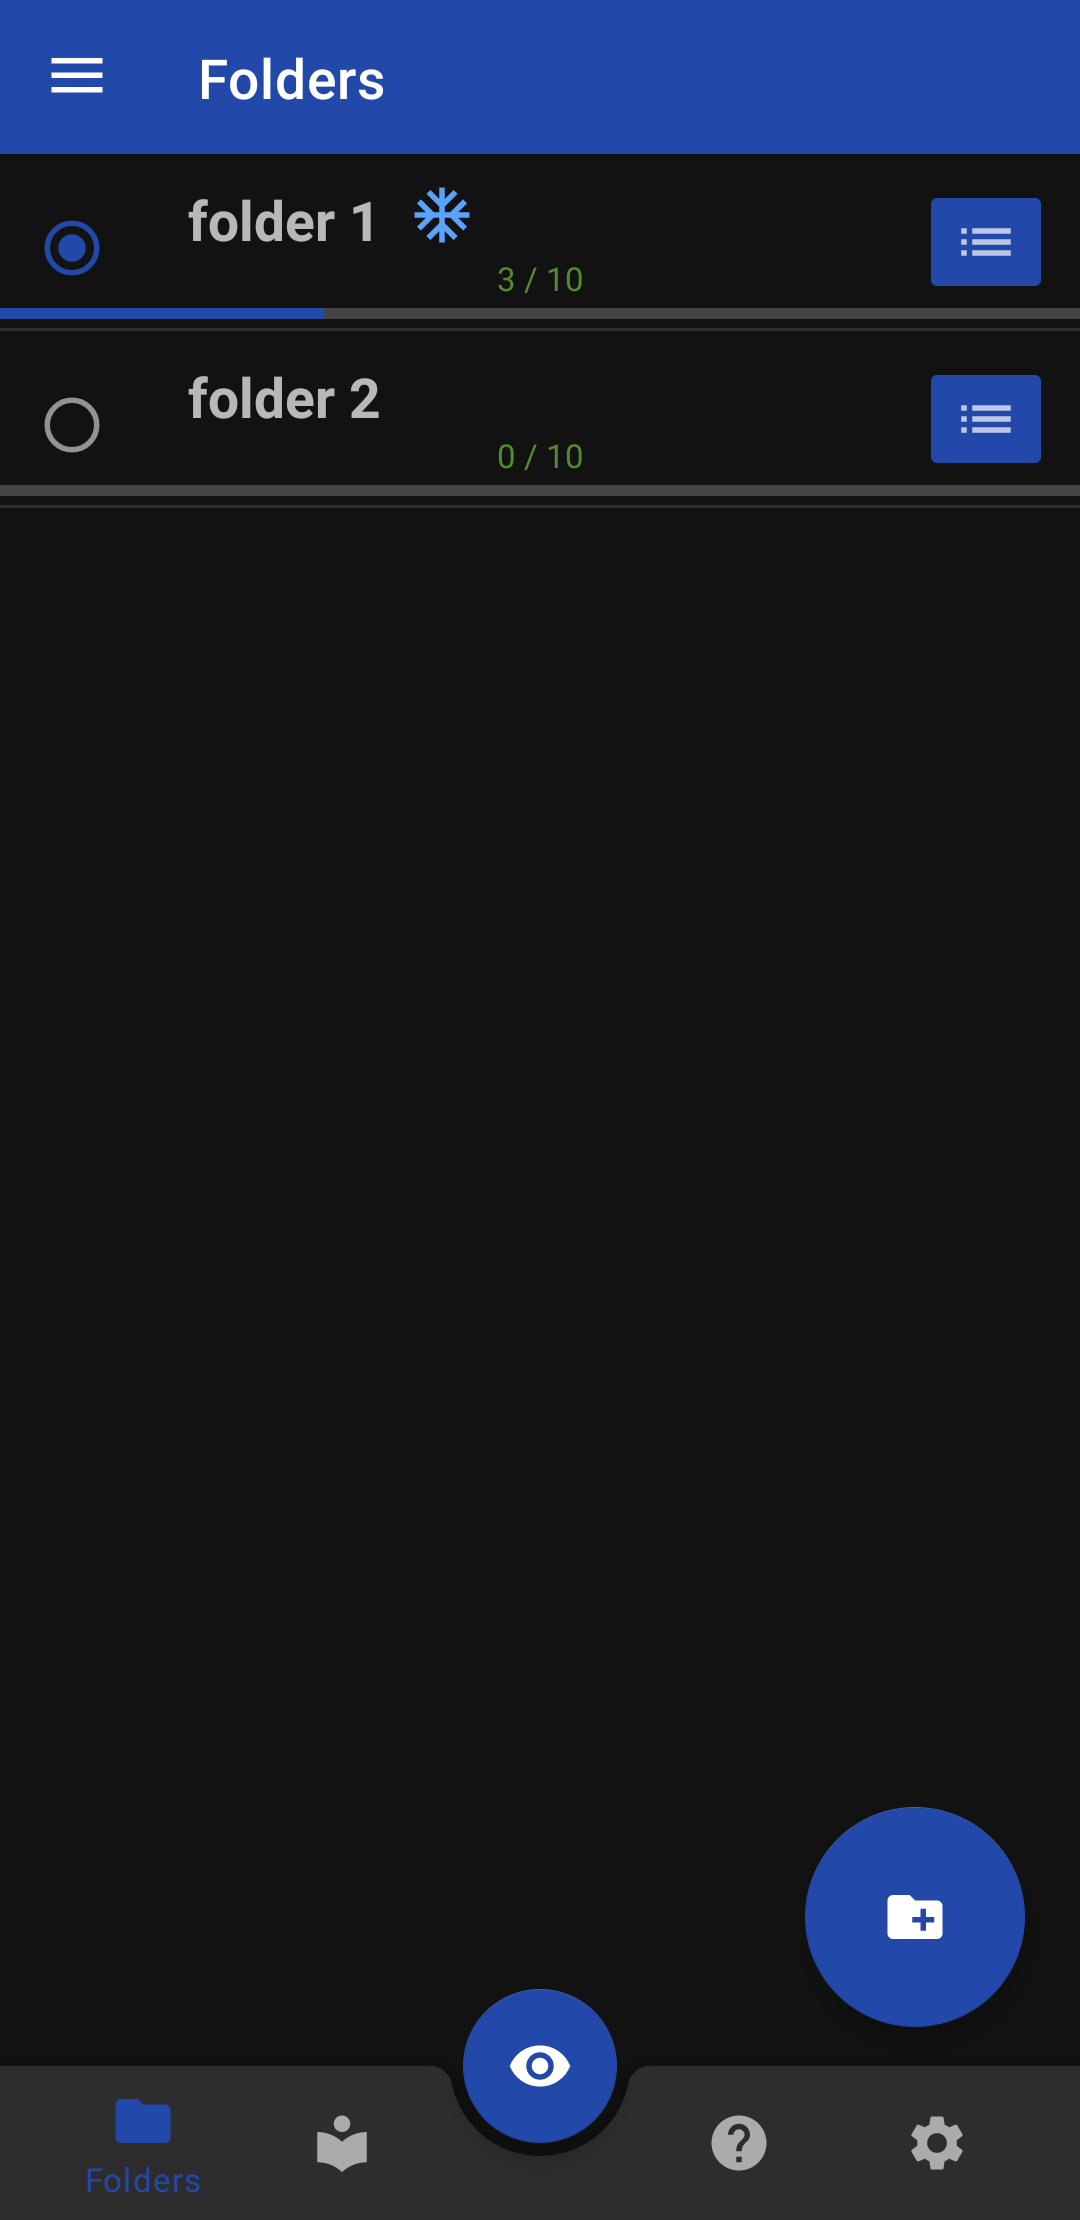
\includegraphics[height=0.6\textheight]{images/screenshots/model-overview.png}
	\caption{Screenshot: Modellübersicht/Objektordner-Übersicht}
	\label{fig:screenshot:model-overview}
\end{figure}

\begin{figure}[hptb]
	\centering
	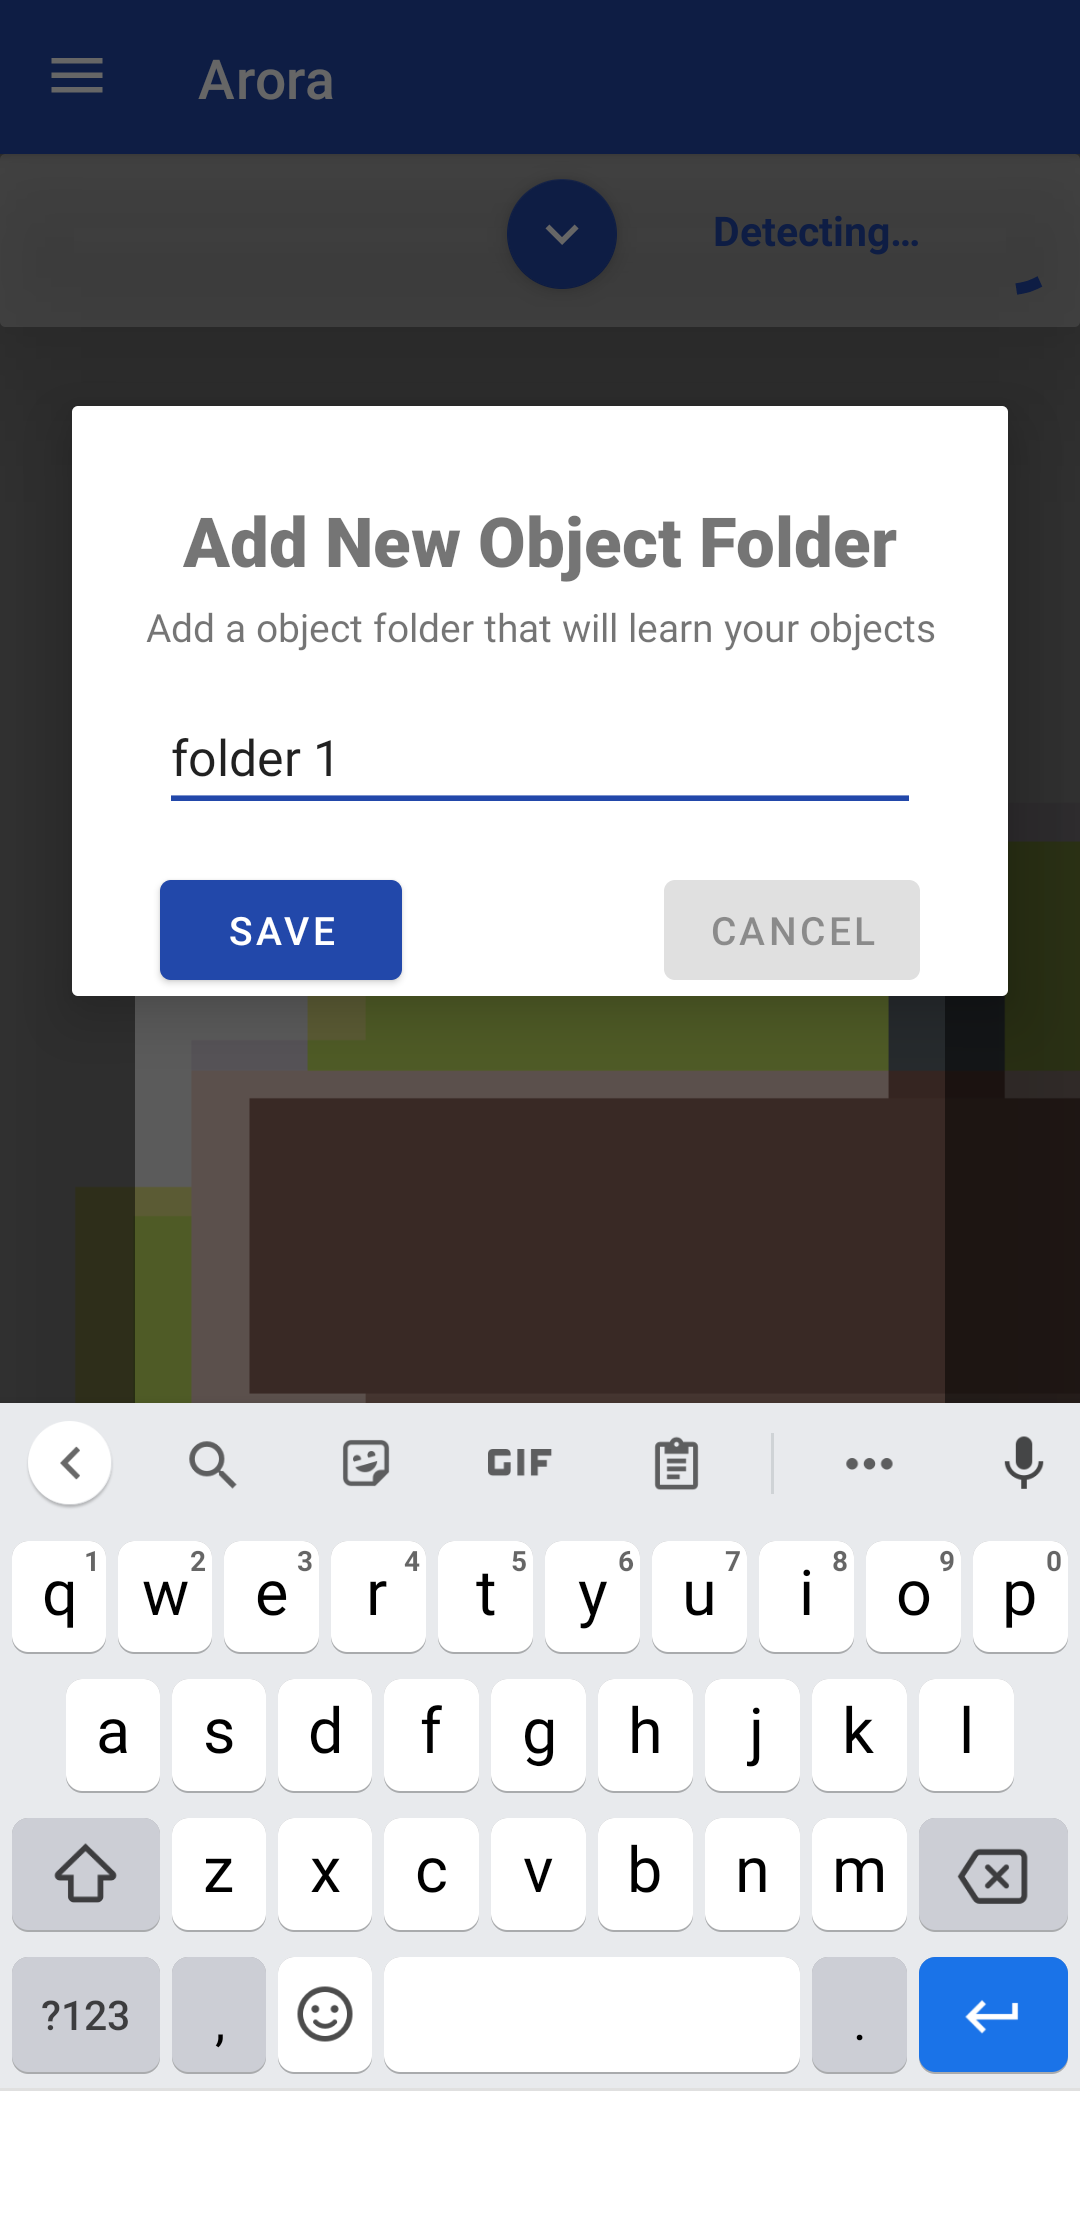
\includegraphics[height=0.6\textheight]{images/screenshots/add-folder.png}
	\caption{Screenshot: Hinzufügen eines Objektordners}
	\label{fig:screenshot:add-model}
\end{figure}

\begin{figure}[hptb]
	\centering
	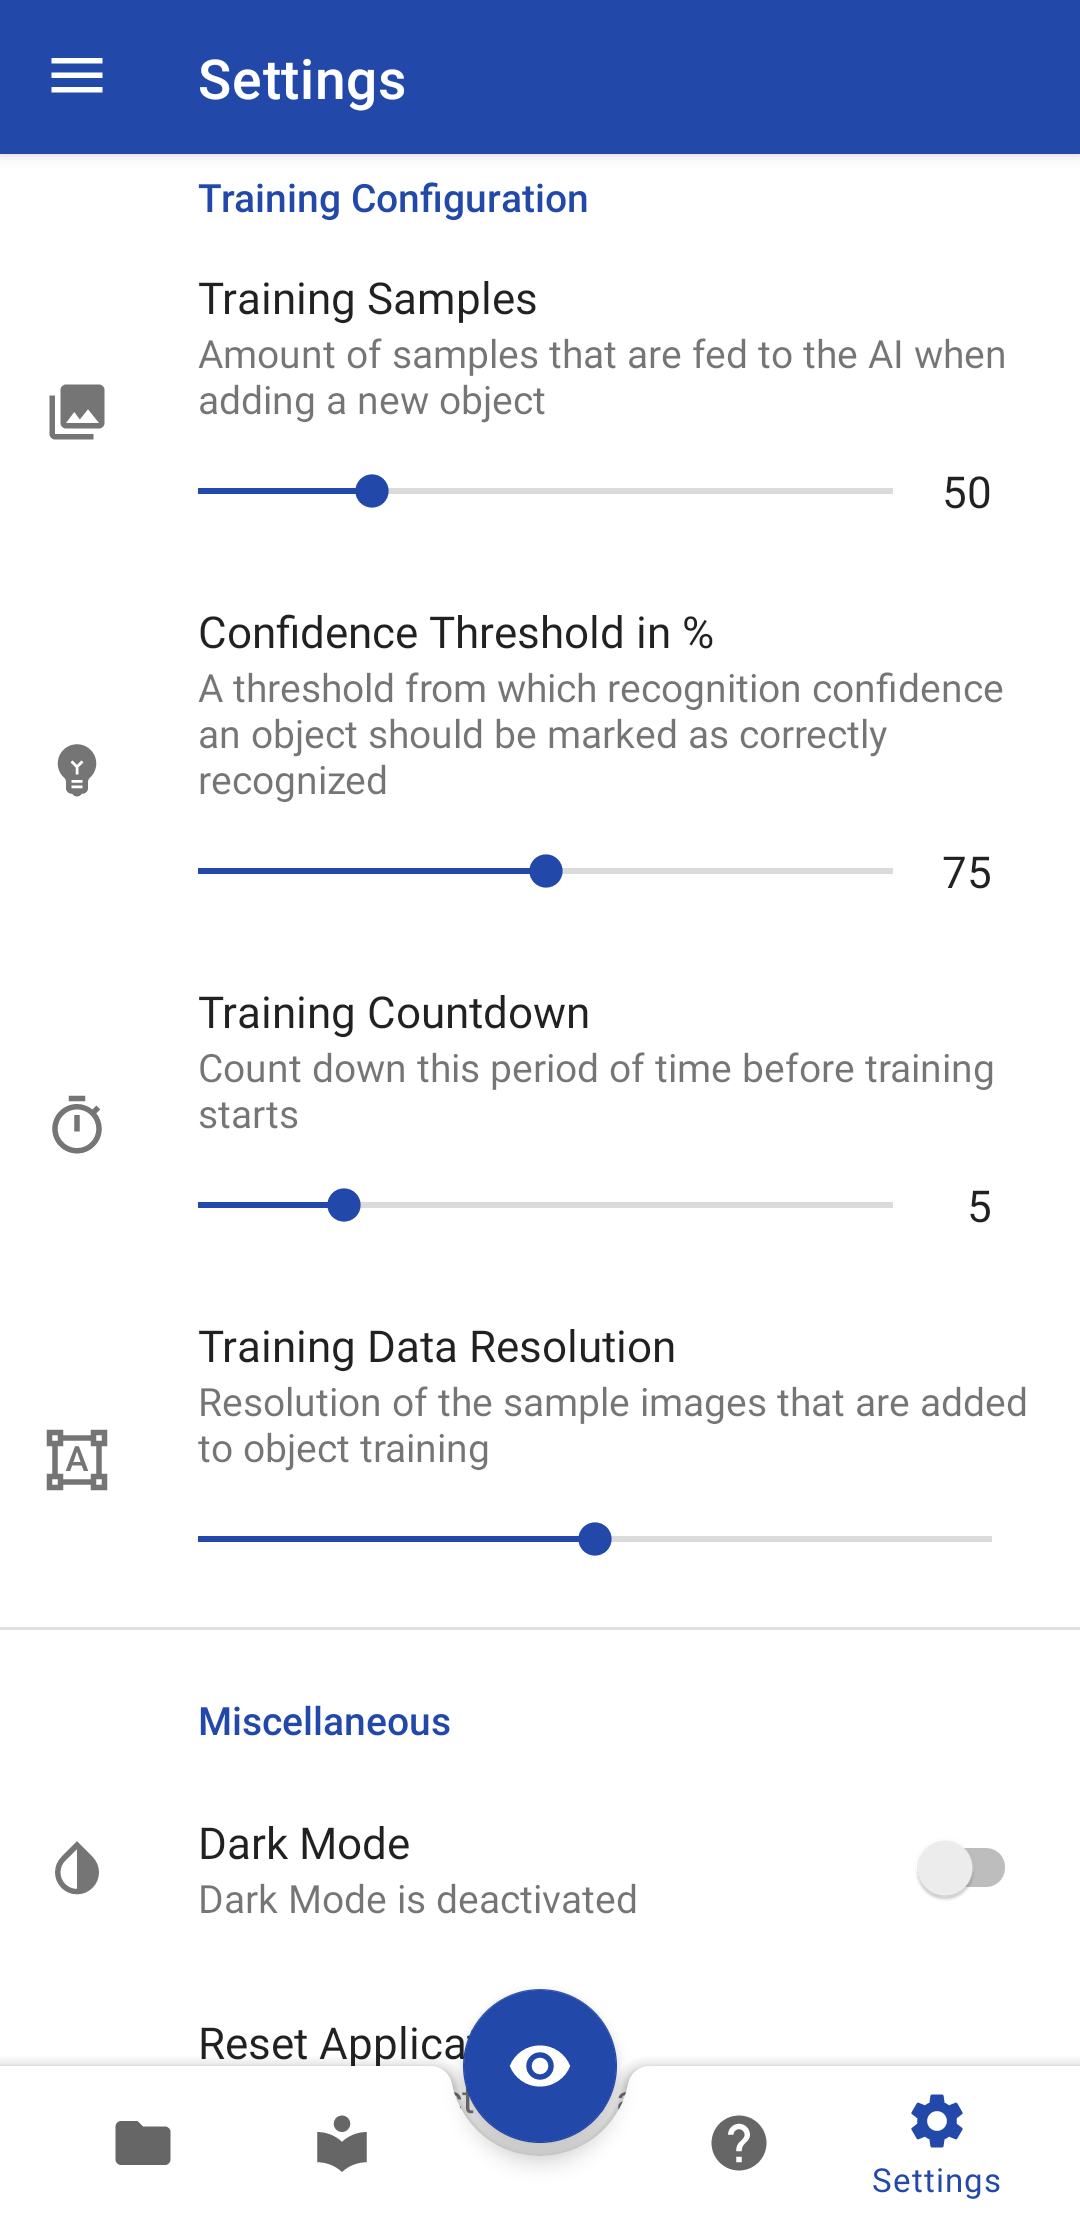
\includegraphics[height=0.6\textheight]{images/screenshots/settings-light.png}
	\caption{Screenshot: Einstellungsansicht im hellen Modus}
	\label{fig:screenshot:settings-light}
\end{figure}

\begin{figure}[hptb]
	\centering
	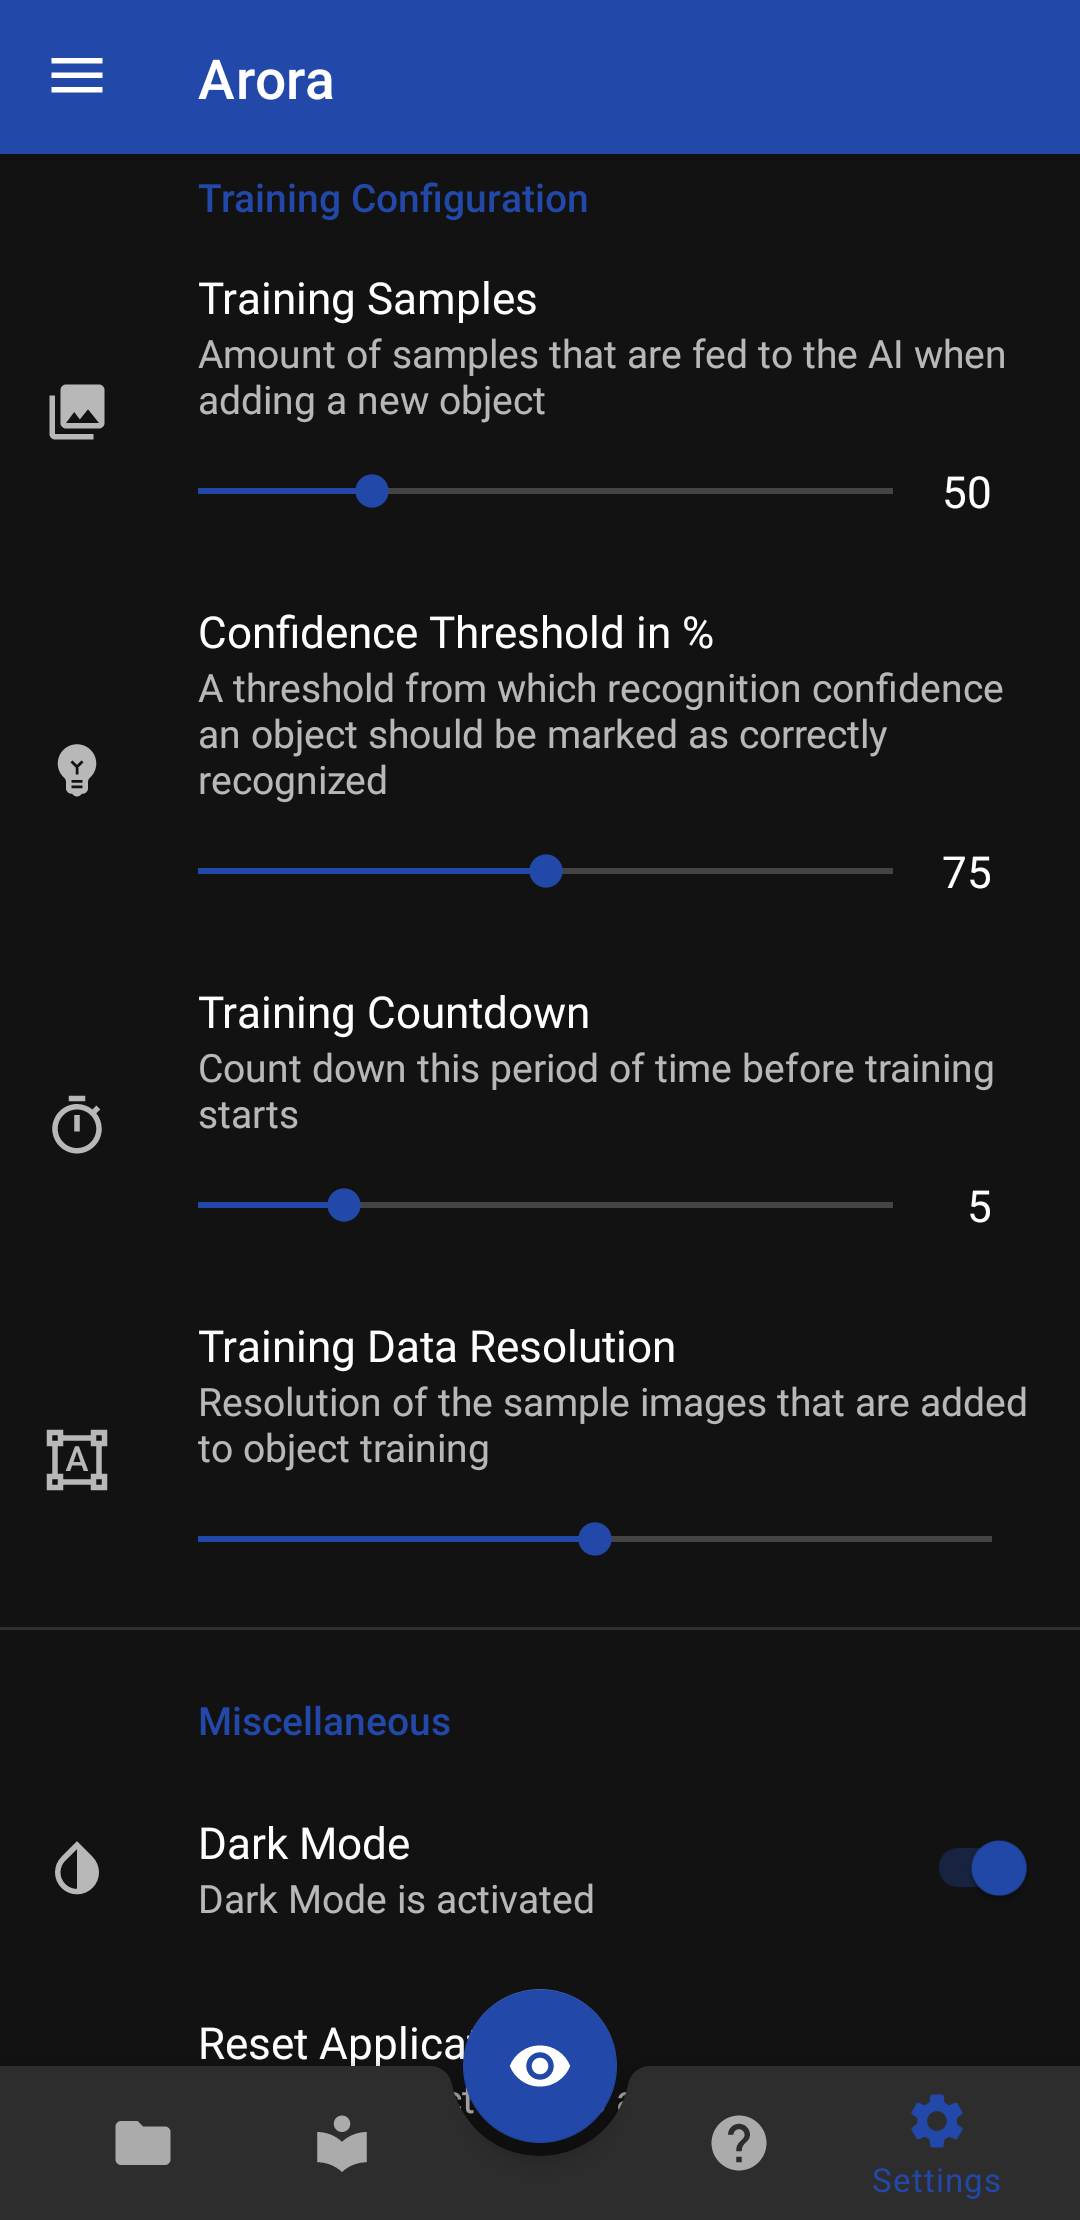
\includegraphics[height=0.6\textheight]{images/screenshots/settings-dark.png}
	\caption{Screenshot: Einstellungsansicht im Dunkelmodus}
	\label{fig:screenshot:settings-dark}
\end{figure}

\begin{figure}[hptb]
	\centering
	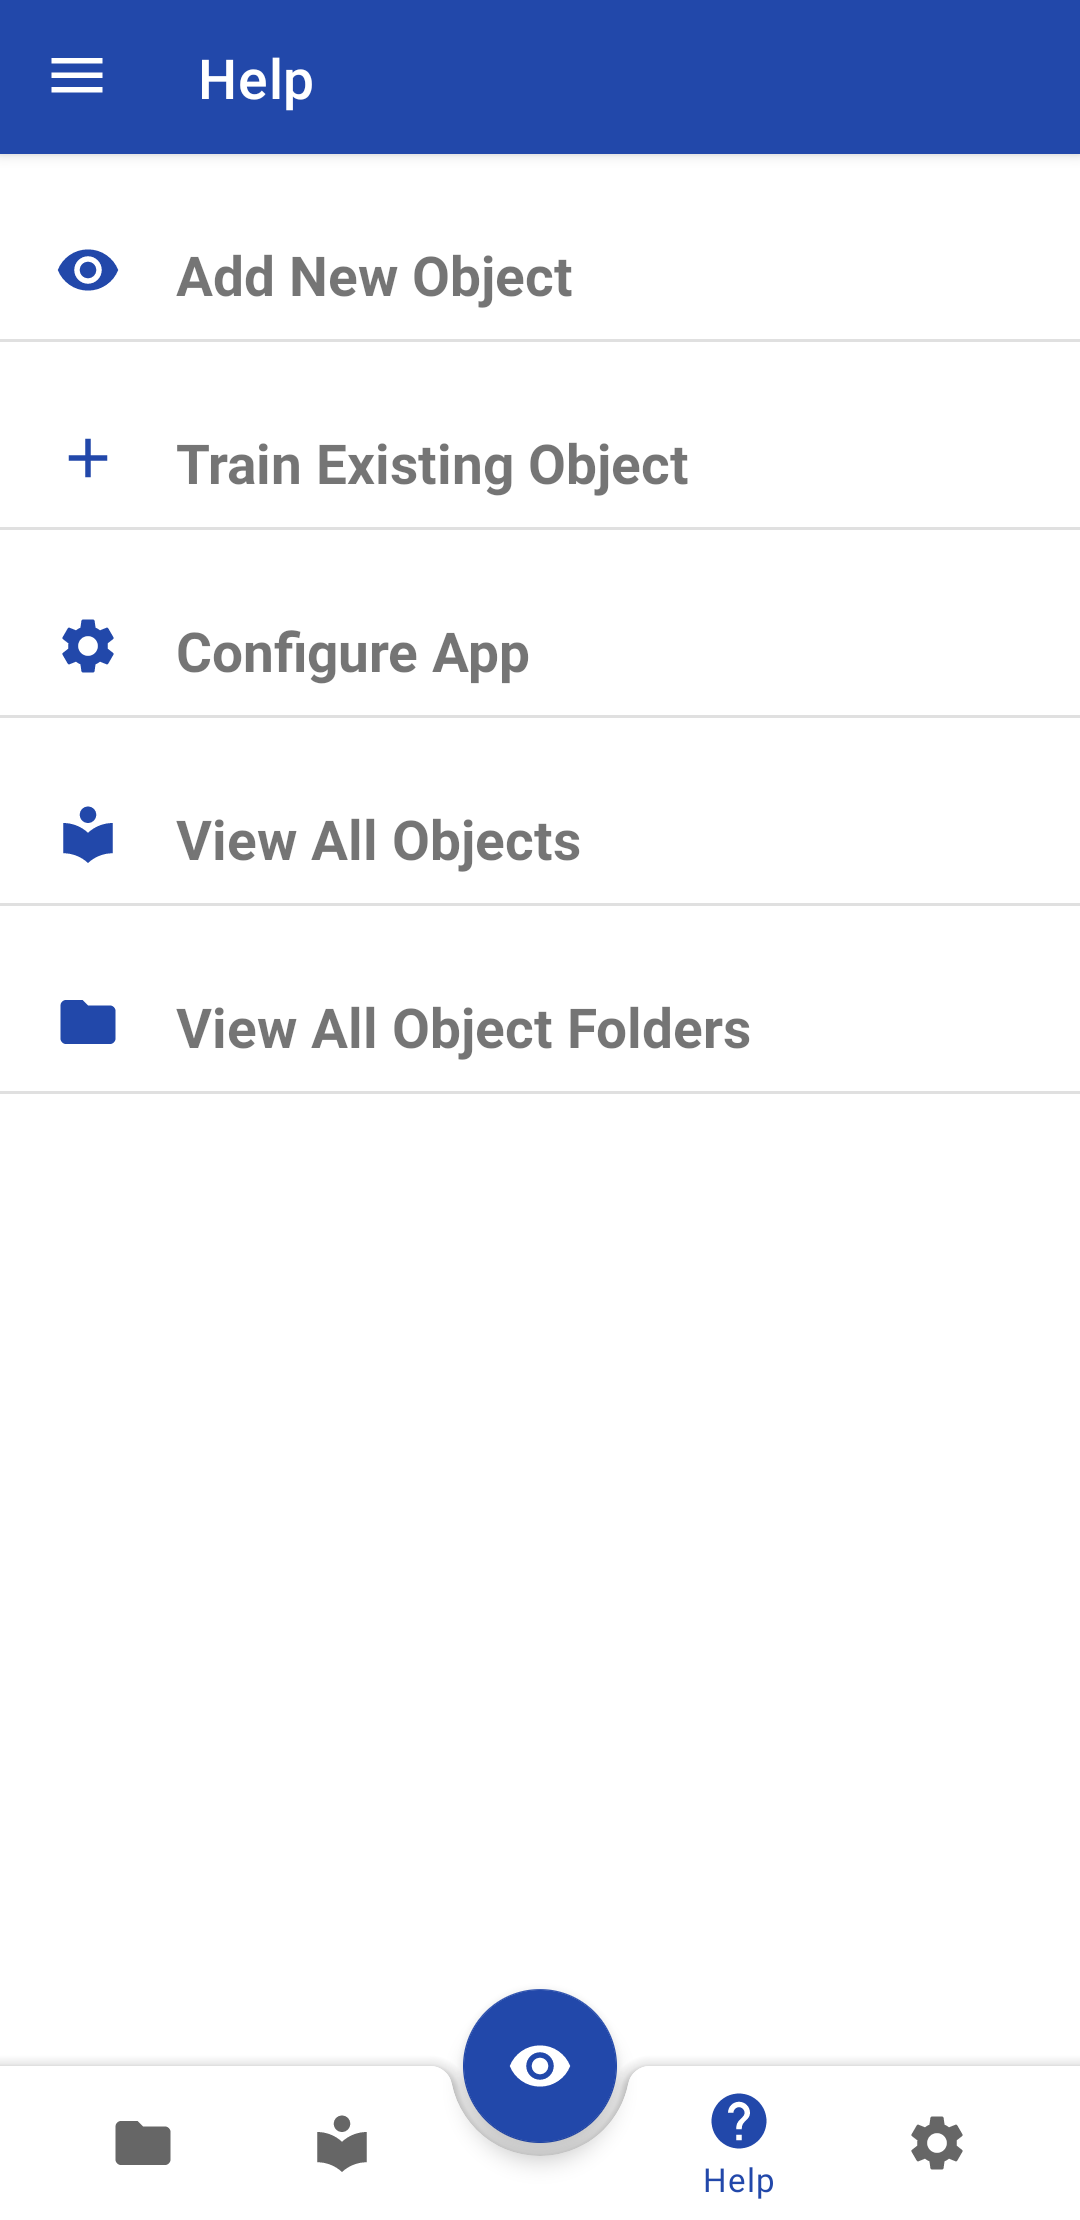
\includegraphics[height=0.6\textheight]{images/screenshots/help-overview.png}
	\caption{Screenshot: Hilfeübersicht}
	\label{fig:screenshot:help-overview}
\end{figure}

\begin{figure}[hptb]
	\centering
	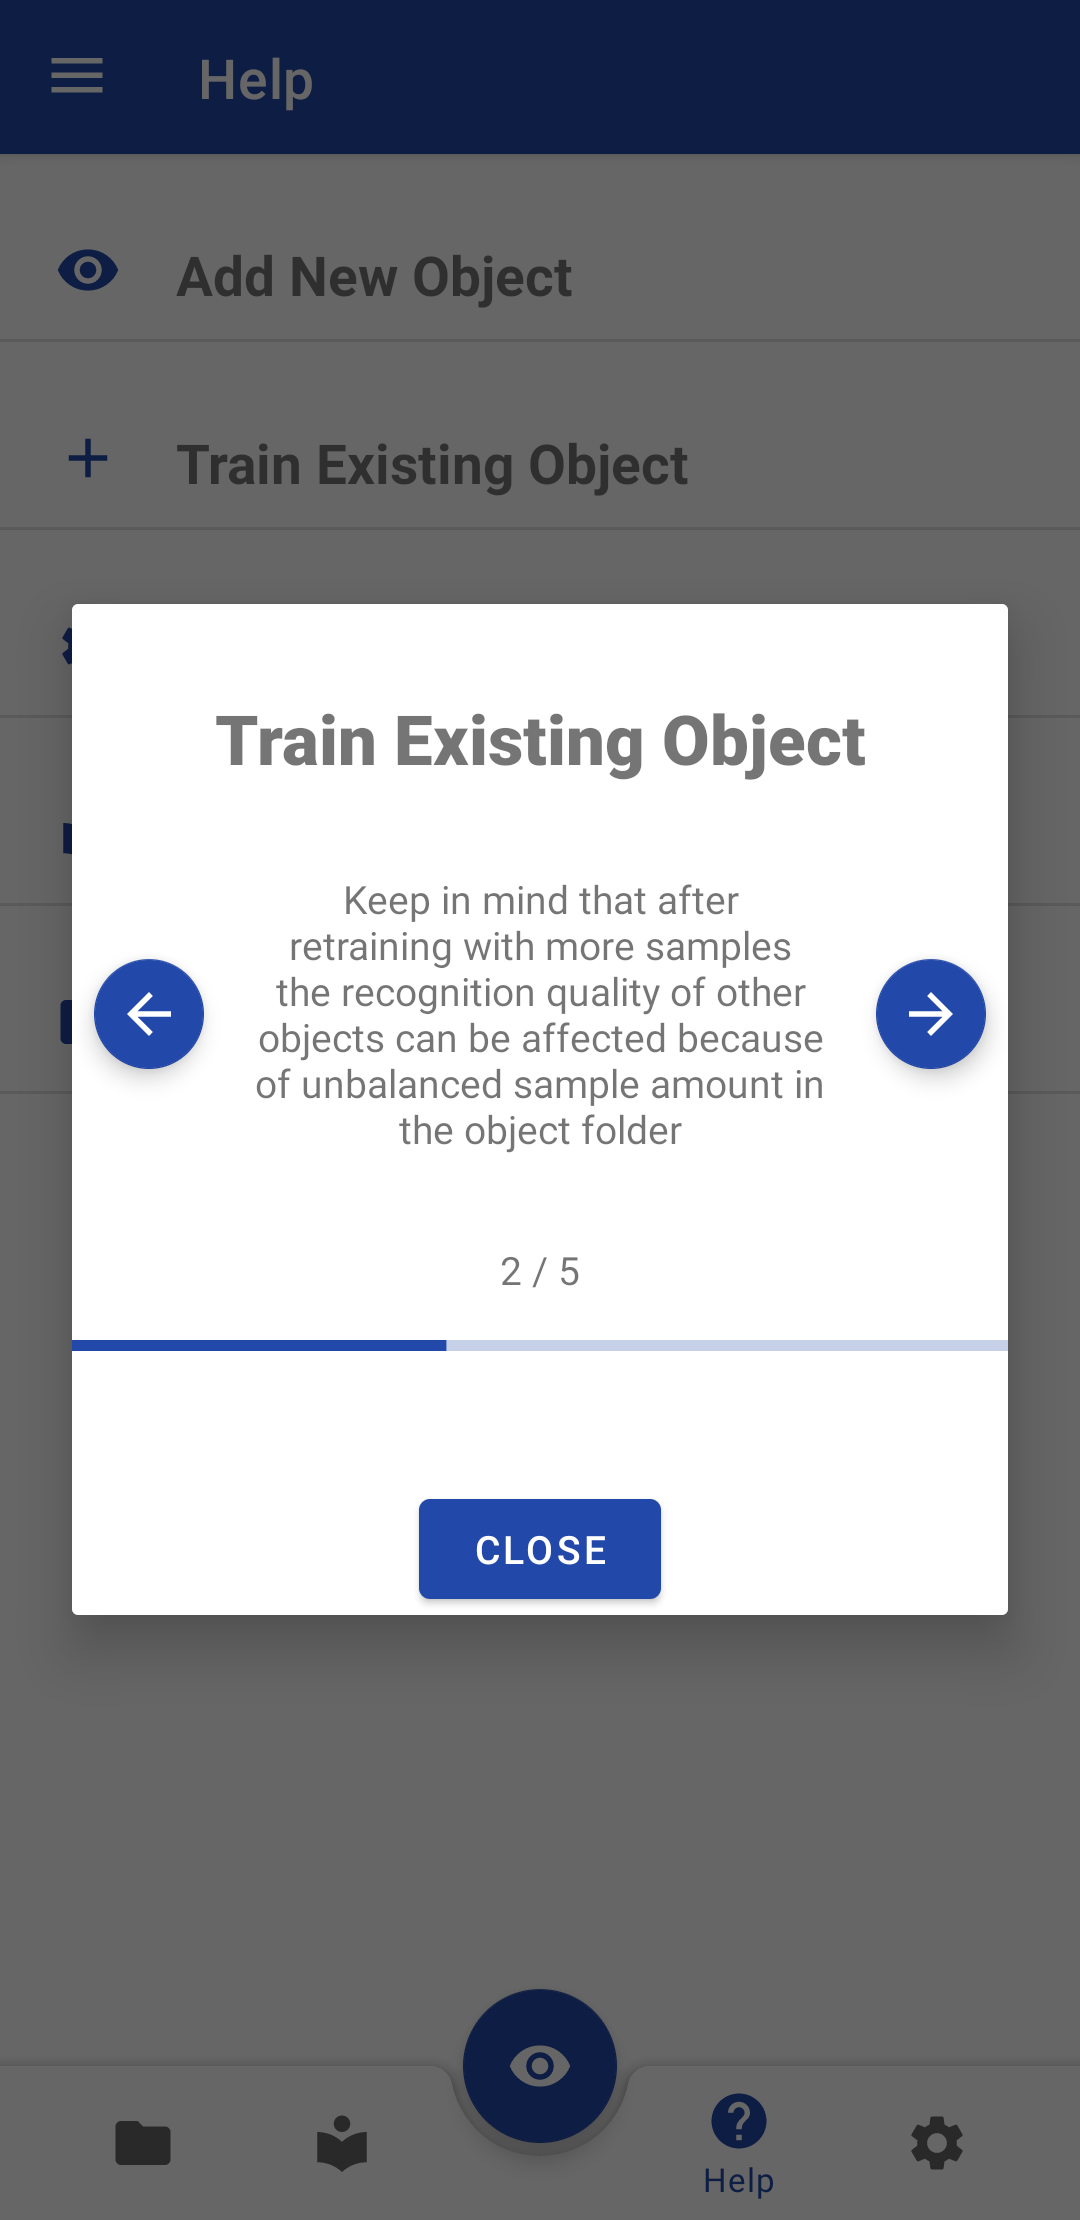
\includegraphics[height=0.6\textheight]{images/screenshots/help-dialog.png}
	\caption{Screenshot: Beispiel eines Hilfedialogs}
	\label{fig:screenshot:help-dialog}
\end{figure}

\begin{figure}[hptb]
	\centering
	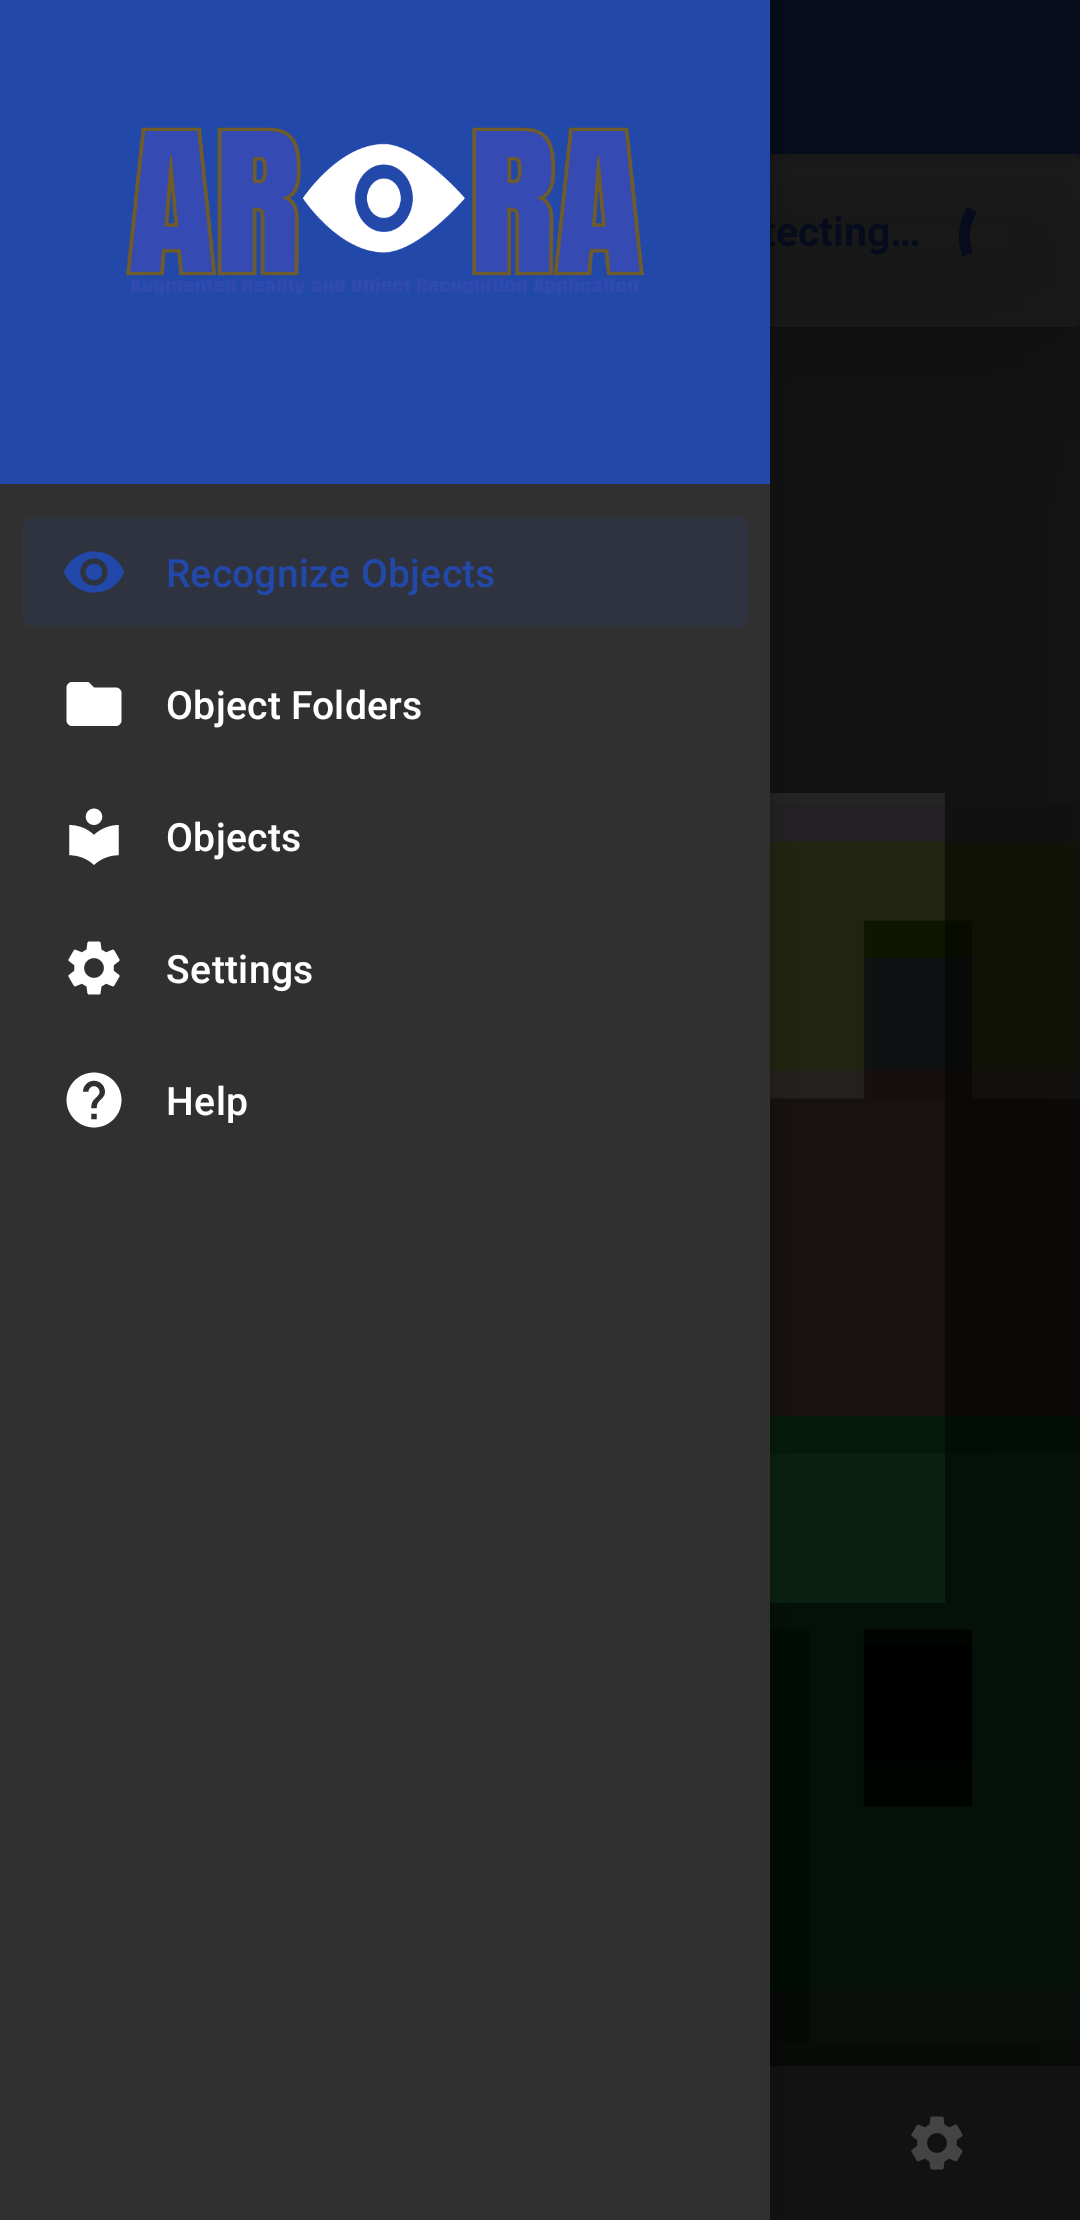
\includegraphics[height=0.6\textheight]{images/screenshots/side-nav.png}
	\caption{Screenshot: Ausklappbare Seitennavigationsleiste}
	\label{fig:screenshot:side-nav}
\end{figure}

\end{document}